% \documentclass[twocolumn]{aastex631}
\documentclass[twocolumn, linenumbers]{aastex631}
%%% Authors to Add: Kate Whitaker, David Setton, Rachel Bezanson, Robert Feldmann, Jenny Green, Wren Suess, Justin Spilker
\raggedbottom
%\documentclass{aastex631}
% \documentclass[linenumbers, twocolumn]{aastex631}
%% The default is a single spaced, 10 point font, single spaced article.
\usepackage{enumitem}
\usepackage{amsmath}
\usepackage{float}
\usepackage{natbib}
\usepackage{cancel}
\usepackage{xcolor,soul}
\usepackage[export]{adjustbox}
\usepackage[normalem]{ulem}
\useunder{\uline}{\ul}{}
%\usepackage{subcaption, graphicx}
\usepackage{hyperref}
\usepackage{bold-extra}
%\bibliographystyle{plainnat}
\usepackage{bm}
\newcommand{\vdag}{(v)^\dagger}
\newcommand\aastex{AAS\TeX}
\newcommand\latex{La\TeX}
\newcommand{\hh}{\text{H}_2}
\newcommand{\fhh}{f_{\text{H}_2}}
\newcommand{\mhh}{M_{\text{H}_2}}
\newcommand{\fgas}{f_{\text{gas}}}
\newcommand{\mgas}{M_{\text{gas}}}
\newcommand{\sfr}{\text{SFR}}
\newcommand{\ssfr}{\text{sSFR}}
\newcommand{\tH}{\text{t}_\text{H}}
\newcommand{\eq}{Eq.\hspace{.2em}}
\renewcommand{\fig}{Fig.\hspace{.2em}}
\renewcommand{\sec}{Sec.\hspace{.2em}}
\newcommand{\app}{Appendix\hspace{.2em}}
\newcommand{\mbh}{M_{\text{BH}}}
\newcommand{\mbhd}{\dot{M}_{\text{BH}}}
\newcommand{\fedd}{f_{\text{Edd}}}
%----------------------------------
\newcommand{\simba}[0]{{\sc simba} }
\newcommand{\mufasa}[0]{{\sc mufasa} }
\newcommand{\yt}[0]{{\sc yt} }
\newcommand{\salad}[0]{{\sc caesar} }
\newcommand{\powderday}[0]{{\sc powderday} }
\newcommand{\hyperion}[0]{{\sc hyperion} }
\newcommand{\fsps}[0]{{\sc fsps} }
\newcommand{\slick}[0]{{\sc slick} }
\newcommand{\gizmo}[0]{{\sc gizmo} }
\newcommand{\eagle}[0]{{\sc eagle} }
\newcommand{\tng}[0]{{\sc IllustrisTNG} }
\newcommand{\shark}[0]{{\sc shark} }
\newcommand{\galform}[0]{{\sc galform} }
\newcommand{\gaea}[0]{{\sc gaea} }
\newcommand{\despotic}[0]{{\sc despotic} }
\newcommand{\magnet}[0]{{\sc Magneticum Pathfinder}}
\newcommand{\aco}{\alpha_\text{CO}}
\newcommand{\acomw}{\alpha_{\text{CO,MW}}}
\newcommand{\lgal}[0]{{\sc L-Galaxies}}
\newcommand{\colibre}[0]{{\sc colibre}}
%{\bfseries \scshape simba}
\newcommand{\red}[1]{{\color{red} #1}} % new text
% \usepackage[dvipsnames]{xcolor}
% \newcommand{\red}[1]{\textcolor{Red}{ \bf #1}} % new text
\newcommand{\blu}[1]{{\color{blue} \bf #1}} %text for ethan to review
%----------------------------------
\graphicspath{{./}{Figures/}{newFigures/}}

\shorttitle{The Mystery of The Red, Dead \& Gassy Galaxies}
\shortauthors{Savitch et al.}
\begin{document}
\title{Unveiling the Origins of the Molecular Gas Reservoirs in Recently Quenched Massive Galaxies}

\author[0000-0002-2919-1109]{Ethan Savitch \href{mailto:esavitch@ufl.edu}{(esavitch@ufl.edu)}}
\affiliation{University of Florida Astronomy, 211 Bryant Space Science Center, Gainesville, FL, 32611, USA}
%\email{esavitch@ufl.edu}

\author[0000-0002-7064-4309]{Desika Narayanan}
\affiliation{University of Florida Astronomy, 211 Bryant Space Science Center, Gainesville, FL, 32611, USA}

\author[0000-0003-4075-7393]{David Setton}
\affiliation{Department of Physics and Astronomy and PITT PACC, University of Pittsburgh, Pittsburgh, PA 15260, USA}

\author[0000-0001-7160-3632]{Kate Whitaker}
\affiliation{Department of Astronomy, University of Massachusetts, Amherst, MA 01003, USA}
\affiliation{Cosmic Dawn Center (DAWN), Niels Bohr Institute, University of Copenhagen, Jagtvej 128, København N, DK-2200, Denmark}

\author[0000-0001-5063-8254]{Rachel Bezanson}
\affiliation{Department of Physics and Astronomy and PITT PACC, University of Pittsburgh, Pittsburgh, PA 15260, USA}

\author[0000-0002-0766-1704]{Elia Cenci}
\affiliation{Department of Astronomy, University of Geneva, Chemin Pegasi 51, Versoix CH-1290, Switzerland}
\affiliation{Department of Astrophysics, Universit\"at Z\"urich, Winterthurerstrasse 190, Zurich CH-8057, Switzerland}

\author[0000-0003-2842-9434]{Romeel Dav\'e}
\affiliation{University of Edinburgh, Institute for Astronomy}

\author[0000-0002-1759-6205]{Vincenzo R. D'Onofrio}
\affiliation{Department of Physics and Astronomy and George P. and Cynthia Woods Mitchell Institute for Fundamental Physics and Astronomy, Texas A\&M University, 4242 TAMU, College Station, TX 77843-4242, USA}

\author[0000-0002-1109-1919]{Robert Feldmann}
\affiliation{Department of Astrophysics, Universit\"at Z\"urich, Winterthurerstrasse 190, Zurich CH-8057, Switzerland}

\author[0000-0002-5612-3427]{Jenny Greene}
\affiliation{Department of Astrophysical Sciences, Princeton University, 4 Ivy Lane, Princeton, NJ 08544, USA}

\author[0000-0002-7613-9872]{Mariska Kriek}
\affiliation{Leiden Observatory, Leiden University, P.O. Box 9513, 2300 RA Leiden, The Netherlands}

\author[0000-0002-9729-3721]{Massimiliano Parente}
\affiliation{University of Florida Astronomy, 211 Bryant Space Science Center, Gainesville, FL, 32611, USA}

\author[0000-0003-3256-5615]{Justin Spilker}
\affiliation{Department of Physics and Astronomy and George P. and Cynthia Woods Mitchell Institute for Fundamental Physics and Astronomy, Texas A\&M University, 4242 TAMU, College Station, TX 77843-4242, USA}

\author[0000-0002-1714-1905]{Katherine A. Suess}
\affiliation{Department for Astrophysical \& Planetary Science, University of Colorado, Boulder, CO 80309, USA}
% \affiliation{Astronomy Department, University of California, Berkeley, CA 94720, USA}

\author[0000-0003-0372-5253]{Dariannette Valentin-Martinez}
\affiliation{University of Florida Astronomy, 211 Bryant Space Science Center, Gainesville, FL, 32611, USA}

\author[0009-0008-7017-5742]{Dhruv Zimmerman}
\affiliation{University of Florida Astronomy, 211 Bryant Space Science Center, Gainesville, FL, 32611, USA}

% KW = Kate Whitaker, MP = Max Parente
\begin{abstract}
Observations of quenched galaxies by standard diagnostics over a range of redshifts have demonstrated examples containing copious reservoirs of molecular gas, which is contrary to the traditional view of gas-poor, red and dead galaxies.  In this study, we employ the \simba cosmological simulation to investigate three possible hypotheses for the origin of molecular gas-rich quenched systems: (i) the inferred quiescence is temporary, and the observed molecular gas will enable the galaxy to rejuvenate; (ii) the abundance of molecular gas stems from an incorrectly assumed CO-to-H$_2$ conversion factor, or (iii) the galaxy is actually star-forming, but the star formation is heavily obscured by dust.  By investigating simulated galaxies from present day out to Cosmic Noon, we find that many seemingly quiescent massive galaxies that are molecular gas-rich are actually hosting dust-obscured star formation, with a visual optical depth $(\tau_V)$ that, on average, increases from 0.9 to 3.7 from $z=0-3$.  Temporary quiescence can occur in gas-rich transitioning galaxies on timescales of around 1-2 Gyr, though this is most prominent at high redshift and is relatively rare overall.  Our model rules out incorrect CO-H$_2$ conversion factors from significantly impacting the inference of $\hh$ gas in quenched galaxies.
\end{abstract}
\keywords{Molecular gas (1037) --- Quenched galaxies (2016) --- Star formation (1596)}
%https://astrothesaurus.org/concept-select/?utm_source=chatgpt.com
% \keywords{galaxies: starburst and star formation --- Molecular Gas --- Star Formation --- Rejuvenation --- Obscuration}
% Quenched galaxies
% \keywords{Quenched Galaxies --- Molecular Gas --- Star Formation --- Rejuvenation --- Obscuration}
%\keywords{Molecular gas (1073), Quenched galaxies (2016), Star formation (1569), Interstellar dust extinction (837)}
% \keywords{Interstellar dust extinction --- Molecular gas --- Quenched galaxies --- Star formation}

%========================== Introduction ==========================
\section{Introduction}
\label{sec:intro}
Observations of galaxies in the local universe find a persistent bimodality in galaxy populations \citep[e.g.][]{noeske,wuyts,Brammer11, Muzzin_2013,jin}.  This dichotomy is defined by one population of star-forming galaxies that are blue in color with spiral morphology \citep{saintonge, tacconi}, and a second population, traditionally called quiescent or `red and dead' galaxies, which have their star formation quenched and have typically early-type morphological structures \citep{blanton03, mcdermid}.  In the Local Universe, star-forming galaxies are observed to be gas-rich relative to their quiescent counterparts \citep{davis,young}.

Studies of massive galaxies at high-$z$ confirm that the majority of quenched systems form their stars early on and in short bursts \citep{carnall, Belli,merlin, suess21, laporte, Tacchella_2022}.  One such product of this rapid quenching are the so-called ``post-starburst galaxies" (hereafter `PSB' galaxies), which are thought to be the direct result of massive galaxies undergoing a strong burst of star formation that dramatically shuts down within $\lesssim$ 1 Gyr \citep{dressler, zabludoff, goto05, goto07, yang, kriek10, wild20, french_2021}.  PSB galaxies are most common at Cosmic Noon, contributing to half of the total growth of quenched galaxies at $z\sim 2$ \citep{Belli}, though they are relatively rare in the local universe, representing only $\sim 20\%$ of transitioning galaxies at $z\sim 1.4$ and a negligible fraction at $z\sim 0$ \citep{tran,whitaker12,wild16, Lotz21,Setton_2023, smercina, park24}. 

Since such galaxies are assumed to be shutting down their star formation and transitioning to being fully quenched, traditional star formation laws suggest that they should be relatively devoid of molecular gas \citep[e.g.][]{Kennicut, shmidt}.  Due to the difficulty of directly observing $\hh$ in distant galaxies, detailed studies of the cold gas reservoirs in PSB galaxies have only become feasible in recent years \citep{rowlands, french_2015, Alatalo, alatalo17,suessSquiggle, setton2025}. Contrary to expectations, such observations have revealed that PSB galaxies can retain significant reservoirs of CO-traced molecular (H$_2$) gas, with molecular gas fractions up to $\sim 20\%$ at $z<1$, even after shutting down their star formation \citep{young, suess_2017, French_2018, Bezanson_2022, Baron22, setton2025, Umehata2025}.  Interestingly, the gas fraction in such galaxies seems to be a strong function of the time since the galaxy has quenched, and the time for such galaxies to deplete their molecular gas is much higher than the time since quenching \citep{suess2025}.  These findings indicate that the quenching of star formation in PSBs is not directly driven by gas exhaustion; instead suggesting that the molecular gas reservoirs are rendered inhospitable to star formation either through the heating or removal of ISM gas.

% recently quenched galaxies at $z<1$ can contain molecular gas fractions up to $\sim 20\%$, similar to star-forming galaxies of similar mass and redshift \citep{suess2025}.

While quenching in such systems has been studied since \citet{dressler}, a clear picture of the processes driving its onset has yet to emerge.  The most commonly proposed mechanisms include processes internal to galaxies (morphological quenching or AGN feedback;\,e.g.,\,\citealt{Martig09, Baron18, Calabro19}) as well as environmental effects like ram-pressure stripping, galaxy mergers, and starvation (e.g.,\! \citealt{blanton09,snyder, Lotz21, Spilker22, Donofrio25}).  However, the timescales associated with many of these mechanisms are not able to account for the rapid quenching observed at high redshift \citep{Yesuf14, french_2017, winds, french_2021, Bezanson_2022}. These questions, along with the difficulty of explaining the large molecular gas abundances detected in such systems \citep[e.g.,][]{YusefHo20, cenci25, setton2025}, pose a challenge for models of galaxy evolution.

Motivated by this, the goal of this paper is to holistically investigate the various proposed pathways that can result in recently quenched high-mass galaxies preserving their molecular gas with cosmological galaxy simulations.  In particular, we investigate three potential physical scenarios for the existence of copious molecular gas reservoirs remaining in massive galaxies with seemingly low star-formation rates.

Our first hypothesis is that recently quenched massive galaxies, with observable levels of molecular gas, may simply be in a temporary period of dormancy, and are on a path to rejuvenation \citep{remus2023,Kimmig25}.  Multiple theoretical studies support this: \cite{Lotz21} found that $\sim23\%$ of massive quiescent galaxies undergo rejuvenation when tracked forward from $z=3.4$ in the \magnet\ simulation suite; \cite{harrold2025} used a semi-analytic model to show that a typical massive and recently quenched galaxy at $z=1$ has a $\sim25\%$ chance of rejuvenating within 1 Gyr; and \cite{colibre} used the new \colibre\ simulations to show that up to half of massive quenched galaxies could rejuvenate after initial quenching.  Observational studies independently support this hypothesis, such as the work by \cite{ellison25} in which FAST 21 cm observations of 68 PSB galaxies were used to show that at low redshift these systems can contain HI gas fractions up to 30\%.  The presence of substantial atomic gas reservoirs observed in these rapidly quenched galaxies suggests that such PSB-like systems do not quench through the wholesale removal of their gas, and therefore remain viable candidates for future rejuvenation.

The remaining two hypotheses we investigate deal with observational effects that could result in the inference of molecular gas present in seemingly quenched galaxies.  Possible solutions could be that the molecular gas is not as abundant as it seems to be (Hypothesis 2), or that the galaxy is not actually as quenched as it appears (Hypothesis 3).  In particular, our second hypothesis investigates whether molecular gas mass estimates are impacted by potentially varying CO-to-H$_2$ conversion factors, and our third hypothesis asks whether dust attenuation mimics colors compatible with selection as a quenched galaxy \citep{uvj, Baron2023, psbEagle, cenci25}.  The latter hypothesis is also supported by evidence that typical massive quenched galaxies at cosmic noon ($z\sim 2.5$) are significantly more reddened than those in the local universe, with dust attenuation falling from $A_V\sim 0.5$ at $z=2.5$ to near zero at present times \citep{siegel24}. 

In \S\ref{sec:methods}, we begin by describing the simulation we use (\S\ref{ssec:simba}), the dust model it implements (\S\ref{sssec:dust}), and the updates to its black hole feedback model (\S\ref{ssec:bh}).  In \S\ref{ssec:prog} we discuss how we track galaxies across different snapshots using progenitor tracking.  Next, in \S\ref{ssec:selectGal} we define our galaxy selection criteria, first focusing on classifying low star-forming galaxies (\S\ref{ssec:select}), then adding on the requirement that systems must be massive and gas-rich (\S\ref{ssec:massLimit}), with the implications of this combined selection discussed in \S\ref{ssec:selectCombined}.  In \S\ref{sec:results}, we present the results of our analysis, with separate subsections for each of the three hypotheses and a final subsection synthesizing the results.  Specifically, in \S\ref{ssec:HA} we examine temporary quiescence, in \S\ref{ssec:HD} the impact of $\aco$, and finally in \S\ref{ssec:HC} we investigate the impact of dust obscuration.  In \S\ref{ssec:allTogether}, we combine insights from the previous sections into a cohesive picture, which we discuss in the context of related observational work.  Next, in \S\ref{sec:discussion}, we discuss how our simulation and methodology compares to other analogous numerical studies.  Finally, in \S\ref{sec:conclusion} we conclude by summarizing our results, their implications, and avenues for future work on this topic.

%========================== Methods ==========================
\section{Methods}
\label{sec:methods}
\subsection{Cosmological Simulations}
\label{ssec:simba}

We employ the \simba galaxy formation simulation \citep{simba}, which is a modern cosmological simulation that includes models for star formation, its associated feedback, black hole growth/feedback, and interstellar dust.  Specifically, we employ the fiducial $(25/$h Mpc)$^3$ box with $512^3$ particles, resulting in a baryon mass resolution of $M_{\rm b} \approx 2\times10^6 M_\odot.$   

The \simba simulation employs the meshless finite mass (MFM) hydrodynamic solver within the \gizmo codebase \citep{hopkins15,hopkins17}.  \simba includes a sub-resolution prescription for star formation and feedback.  Here, star formation occurs stochastically in H$_2$ gas, where the molecular content is determined using the \citet*{KMT07} algorithm, which calculates the fraction of gas in molecular hydrogen ($f_{\hh}\equiv \mhh/\mgas$) as a function of metallicity and column density \citep{mufasa}.  More information about this algorithm can be found in \cite{KMT11} and \cite{thompson}.

Star formation follows a volumetric \citet{shmidt} law (hereafter SFR $\equiv\dot{M}_*=$ Star Formation Rate): 
\begin{equation}
\sfr\equiv \epsilon_*\bigg(\frac{\rho_{\rm gas}\times  \fhh}{t_{\rm ff}}\bigg)\propto \rho_{\rm gas}^{3/2}
\label{eq:sfr}
\end{equation}
where $\epsilon_*=0.02$ is the efficiency of star-formation per free-fall time, and $t_{\rm ff}$ is the free-fall time-scale ($t_{\rm ff}=\sqrt{3\pi/(32G\rho_{\rm gas})} \propto \rho_{\rm gas}^{-1/2}$).  By construction, the star-formation rate is directly dependent on the density of its gas ($\rho_{\rm gas}$), and its molecular gas fraction ($\fhh$).  As a result of this, the simulation also imposes a minimum molecular gas density required for the gas to be able to produce stars \citep{mufasa}, defined as
\begin{equation}\rho_{\hh}\equiv m_{\hh}\times n_{\hh}\equiv \rho_{\rm gas}\times f_{\hh}\geq 0.13\ m_{\hh}/cm^3\label{eq:minDen}\end{equation}

\subsubsection{Dust Model}
\label{sssec:dust}
In addition to the molecular gas and star formation models, \simba also includes an algorithm for dust physics that is able to capture the formation and evolution of cosmic dust.  Due to the inability to resolve gas drag in our simulation, along with the very short time scales associated with it, the model has dust passively follow the flow of gas particles. The modeled dust grains have a single fixed radius of $a=0.1~\mu \text{m}$ (i.e. no evolving dust grain size distribution), and active dust cooling is ignored \citep{simba}.

Following the prescription of \cite{dwek}, dust particles are produced by metal condensation in the ejecta of supernovae (SNe) and AGB stars.  After being produced, the model allows dust to grow in mass by accreting gas-phase metals; in which dust particles collide with gaseous metals, causing the metals to stick to the dust grains and allowing their mass to grow.  In addition, thermal sputtering is implemented so that dust grains can be eroded by thermally excited gas  \citep{simba}.  Finally, since the simulation cannot resolve individual supernovae (SNe) shocks, an additional dust destruction mechanism by SNe shocks is included, following the prescription from \cite{mckinnon}.  The dust model, fully detailed in \cite{Li2019}, shows good agreement with observational constraints on dust abundance, especially its redshift evolution \citep{parente2025}.

\subsubsection{Black Hole Model}
\label{ssec:bh}
\simba implements a black hole growth model following \cite{bhtorque} to simulate accretion from cold gas.  These accreting black holes impart feedback into the surrounding ISM, incorporated via a kinetic subgrid model for black holes, along with energetic feedback from X-rays \citep{simba}.  The model for black hole growth is parameterized principally in terms of the Eddington ratio, $\fedd\equiv \mbhd/\dot{M}_{\text{Edd}}$, defined as the ratio of the black hole's accretion rate ($\mbhd$) to the Eddington accretion rate ($\dot{M}_{\text{Edd}}$).  

Since any galaxy can contain more than one supermassive black hole (e.g. due to mergers), the primary (`central') black hole for which the Eddington fraction is computed is defined as the most massive black hole in the galaxy, which at every time step is repositioned at the location of the global minimum of its host galaxy's potential well based on the assumption of efficient dynamical friction \citep{simba}.  If more than two black holes are located within a single black hole kernel size, then they are allowed to merge instantaneously if their relative velocity is lower than three themes their mutual escape velocity \citep{simba}.  


The bolometric luminosity of the resulting AGN is proportional to its accretion rate, $L_{\text{BH}}=\epsilon_{\text{f}}\mbhd c^2$, where $\epsilon_\text{f}=0.1$ is the radiative efficiency of its feedback.



The amount of material that is finally ejected by the AGN is then calculated in order to obtain a momentum output of $\dot{P}_{\text{out}}=20L_{\text{BH}}/c$.  Motivated by observations of AGN outflows and their momentum and energy inputs \citep{Fiore2017}, the value of 20 was chosen to achieve the desired mass loading factor relative to the black hole accretion rate.


% Since any galaxy can contain more than one supermassive black hole (e.g. due to mergers), the primary (`central') black hole for which the Eddington fraction is computed is defined as the most massive black hole in the galaxy, which can change across redshift.  Furthermore, at every time step, this most massive black hole is repositioned at the location of the global minimum of its host galaxy's potential well \citep{simba}.

% The bolometric luminosity of the resulting AGN is proportional to its accretion rate, $L_{\text{BH}}=\epsilon_{\text{f}}\mbhd c^2$, where $\epsilon_\text{f}=0.1$ is the radiative efficiency of its feedback.  The amount of material that is finally ejected by the AGN is then calculated in order to obtain a momentum output of $\dot{P}_{\text{out}}=20L_{\text{BH}}/c$.  Motivated by observations of AGN outflows and their momentum and energy inputs \citep{Fiore2017}, the value of 20 was chosen to achieve the desired mass loading factor relative to the black hole accretion rate.

Similarly, the Eddington accretion rate ($\dot{M}_{\text{Edd}}$) can be defined in terms of the Eddington luminosity: $L_{\text{Edd}}=4\pi G\mbh cm_p/\sigma_T=\epsilon_{\text{f}} \dot{M}_{\text{Edd}}c^2$ \citep{Thomas_2019}, where $\mbh$ is the mass of the primary black hole.  This allows us to re-express the Eddington fraction as: 
\begin{equation}
    \fedd\equiv \frac{\mbhd}{\dot{M}_{\text{Edd}}}=\left(\frac{\epsilon_\text{f} \sigma_T c}{4\pi Gm_p}\right)\frac{\mbhd}{\mbh}\label{eq:fedd}
\end{equation}
Evaluating the leading constants gives $\epsilon_\text{f} \sigma_T c/4\pi Gm_p\approx 4.5\times 10^7$ yr.  Thus, expressing the Eddington ratio in terms of the parameters stated above in \eq \ref{eq:fedd} allows us to calculate it using easily accessible simulation parameters that describe the black hole particles' properties. 

In total, the simulation has three modes of black hole feedback \citep{simba}, defined below:
\begin{itemize}[leftmargin=*]
\item[(1)] The default mode for black hole feedback at early times (high redshift) is the `radiative mode', which occurs in galaxies whose central black holes have Eddington fractions greater than 20\% $(\fedd>0.2)$.  In this mode, the AGNs drive multiphase winds that include warm and ionized gas at a velocity that is dependent on the black holes' mass.

\item[(2)] The next black hole feedback regime is the `jet mode', and in order to be triggered requires two conditions.  First, the Eddington fraction must have dropped below $20\%$ (so that $\fedd<0.2$).  Second, a minimum black hole mass is required, set conservatively at $10^{7.5}M_\odot$.  Thus, if the most massive black hole in a galaxy has both $\fedd<0.2$ \textit{and} $\mbh>10^{7.5}M_\odot$, then the jet mode is triggered in which the AGN drives mostly hot gas in collimated jets, at a velocity that increases as $\fedd$ drops.  This jet velocity is added to the radiative mode velocity, speeding them at most by an additional 7000 km/s when $\fedd=0.02$, at which point the velocity is capped.


\item[(3)] The final mode of black hole feedback is the `X-ray mode', which is triggered when both (i) the Eddington fraction decreases below 2\% $(\fedd<0.02)$ and (ii) the gas fraction, defined as $\fgas\equiv \mgas/M_{*}$, is less than 20\% $(\fgas<0.2)$.  When both conditions are met, the galaxies' accretion disk will radiate the surrounding gas via X-ray heating, providing a radial kick outwards and an increase in temperature.
\end{itemize}

While the `radiative mode' does not have a strong effect on the large-scale properties of the simulation, it can provide a small amount of feedback in star-forming galaxies \citep{dave20}.  In contrast, the ejective `jet mode' triggered next plays a critical role in suppressing star formation and maintaining the population of all quenched galaxies at low redshift.  Finally, the `X-ray mode' is triggered, and while its effects are minimal in determining the galaxy mass function, it provides a crucial additional energy source necessary for fully quenching the star formation of massive galaxies \citep{simba}.  In these cases, the corresponding halo mass causes a hot gaseous halo to form around the system, which shuts off the inflow of fresh gas, eventually quenching the galaxy \citep{Hardcastle07}.

\subsection{Progenitor/Descendant Tracking}
\label{ssec:prog}
%  \salad is a \yt\!\!-based package \citep{yt}, which identifies galaxies using a 6D friends-of-friends algorithm with a spatial linking length of 0.0056 times the mean interparticle separation, and a velocity linking length set to the local velocity dispersion. 

After the execution of the \simba simulation, we employ \salad \citep{salad}, a \yt\!\!-based package \citep{yt}, to identify dark-matter halos and galaxies using a 6D friends-of-friends algorithm.  For each snapshot, \salad outputs a cross-matched halo and galaxy HDF5 catalog, with an abundance of precomputed properties for each \citep{simba}, as well as the particle data used to calculate them.  The resulting catalog from \salad further orders galaxies according to their total stellar mass, so that the 5th galaxy in the list is the 5th most massive at that snapshot.  As a result of this mass-ranked ordering scheme, in order to track a single galaxy through time, we must have an external module for linking galaxies across multiple snapshots, which is achieved via a method called ``progenitor/descendant tracking", which links galaxies through time based on their shared star particles.


In order to track a single galaxy backwards through time (to higher $z$) we must use progenitor tracking.  Since any one galaxy would have had many ancestral galaxies that merged to produce it, tracking galaxies backwards in time requires following \textit{all} galaxies that share common star particles with it at any point in the past, similar to how a humans' genetic makeup is a combination of those of their grandparents.  In practice, we identify a galaxy of interest at $z=0$, and then increment through successive higher redshift snapshots, searching for all galaxies that share at least $10\%$ star particles in common with our galaxy of interest, all of which will be considered its progenitors.  Since all such galaxies will eventually contribute to our target galaxy at $z=0$, we must sum up \textit{all} of their properties to effectively compare across snapshots.  Conceptually, this is essentially calculating the merger tree for any target galaxy, with increasing nodes at higher redshift.  This formalism arises from the fact that mergers occur as galaxies grow and evolve. 


While this method works for moving backward in time, if we wanted to track a galaxy forward in time (to lower $z$) we would instead be tracking its descendants.  This becomes necessary, for example, when we want to see at a given redshift if a galaxy will rejuvenate as time increases.  As discussed in the literature \citep[e.g.][]{Torrey_2015}, this process is fundamentally different from progenitor tracking due to the nature of mergers.  While tracking a galaxy backwards in time using a merger tree requires calculating the sum of all the progenitors, tracking it forward in time requires only the most massive parent node to be tracked up the tree.  This is because while tracking galaxies forward in time a significant fraction of the population can be `lost' via merger events, no such loss occurs when tracking backward in time \citep{Torrey_2015}.

\subsection{Galaxy Selection Criteria}
\label{ssec:selectGal}
After running the \simba \citep{simba} simulation, \salad \citep{salad} is employed in post-processing to identify all available galaxies.  Before requiring any selection criteria, our original sample has $\sim$20,800 galaxies at $z=0$, $\sim$13,200 at $z=1$, and $\sim$8,700 at $z=2$.
\begin{figure*}[htb!]
    \centering
    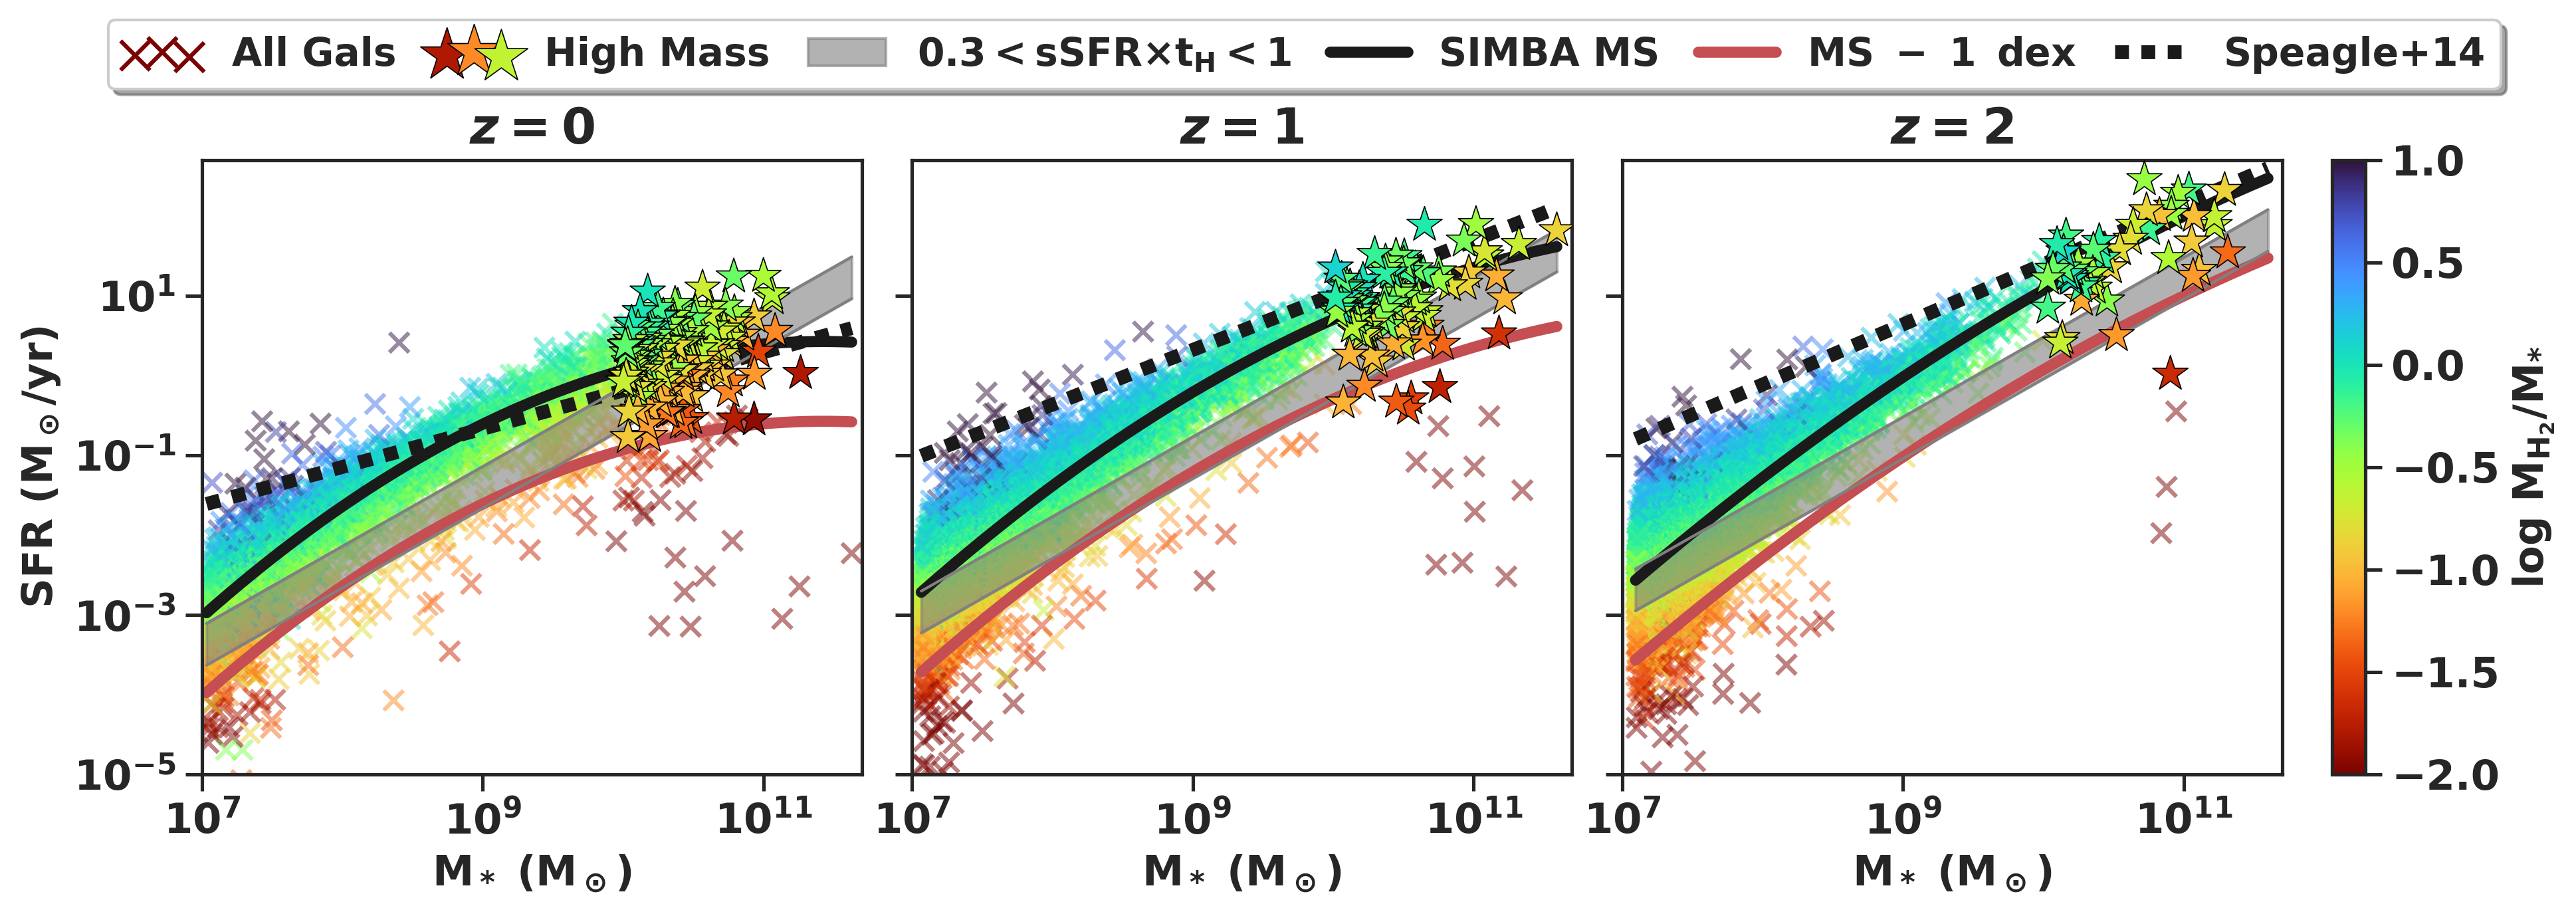
\includegraphics[width=2\columnwidth]{fig1_SFMS_V2.png}
    %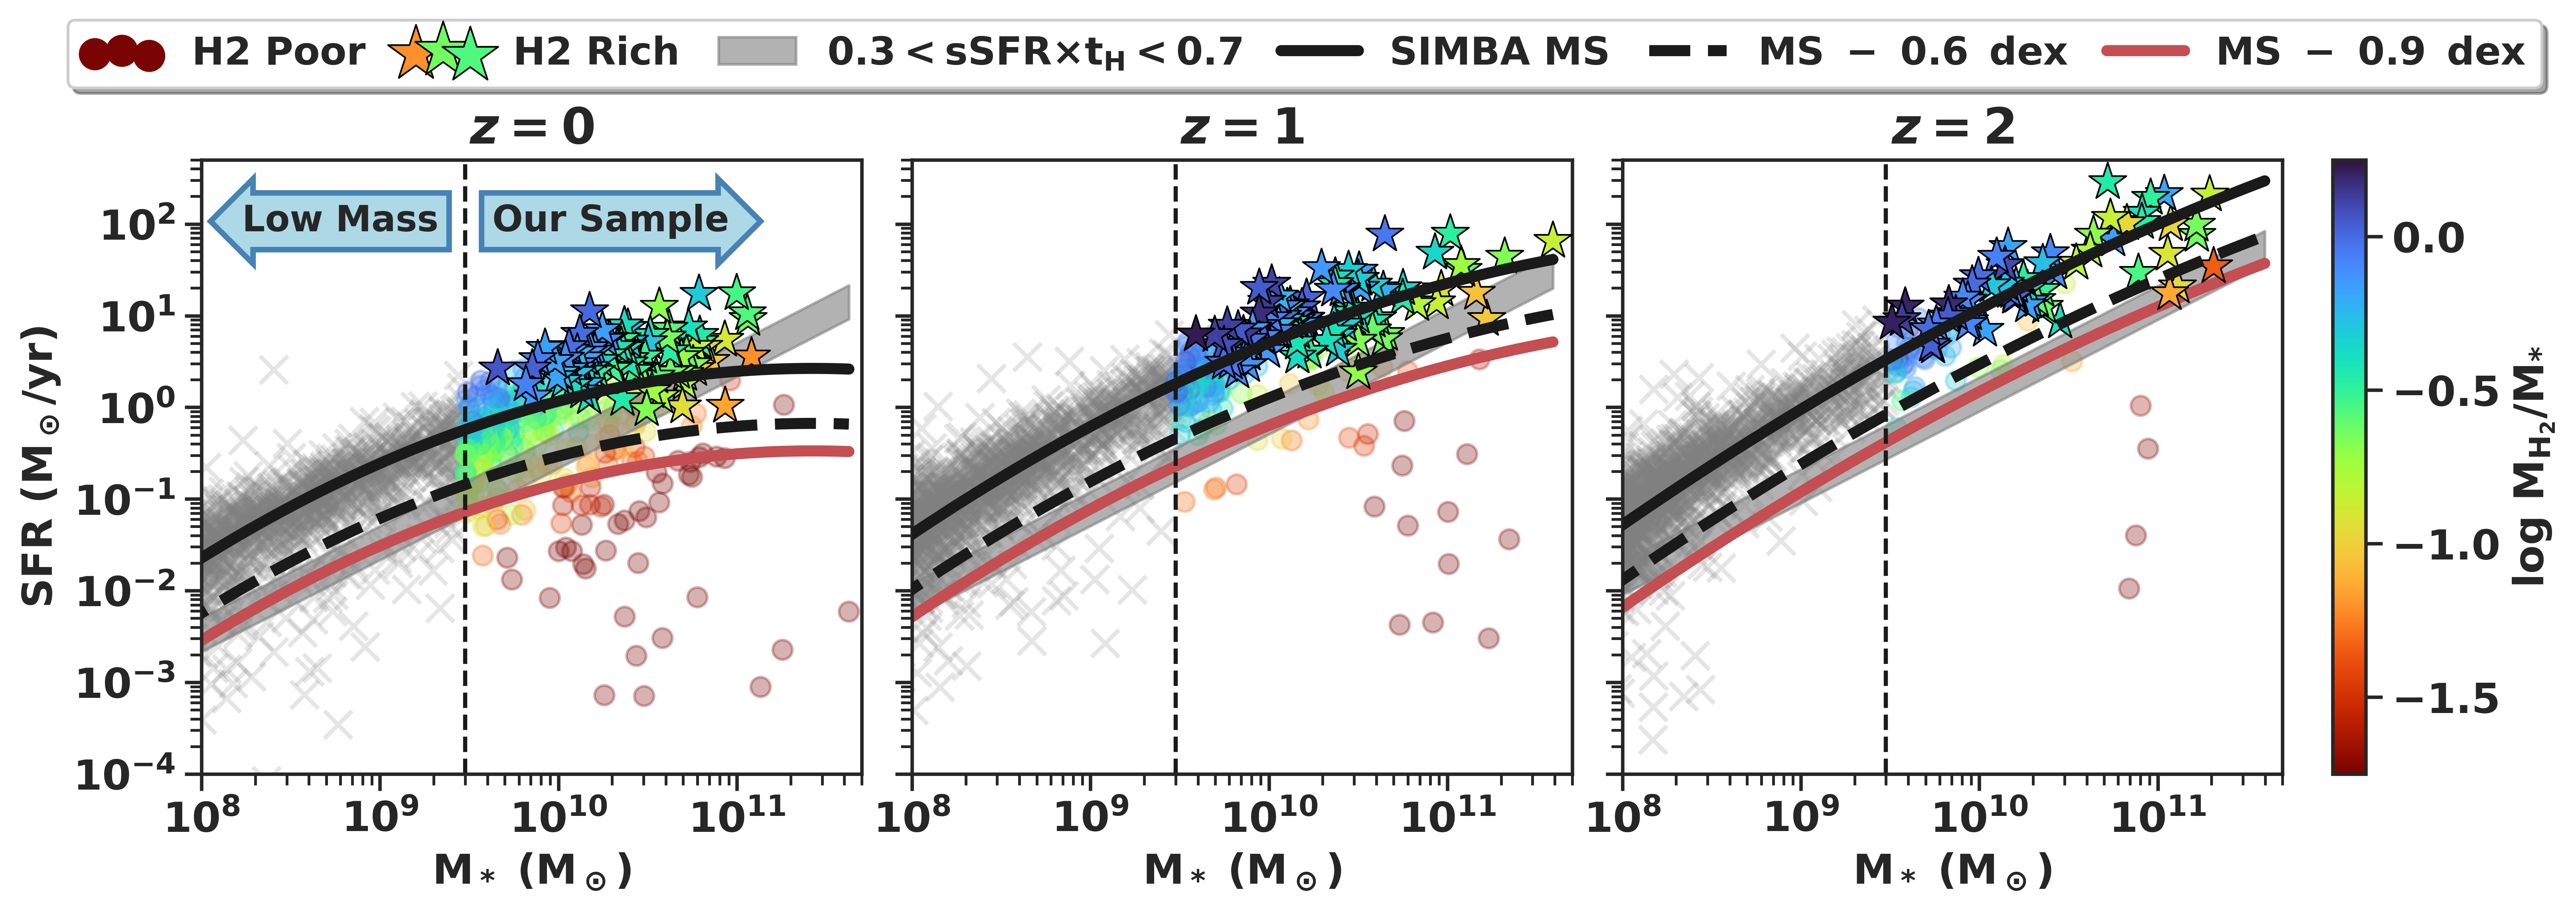
\includegraphics[width=2\columnwidth]{newFigures/fig1_SFMS_newClass.png}
      \caption{{\bf Full galaxy sample shown along with our adopted selection criteria, as well as alternate methods.}  Each point represents a galaxy in our \simba simulation, shown as a star if it satisfies our `high mass' requirement (\S\ref{ssec:massLimit}; \eq\ref{eq:massLimit}) and a cross if not, with a color corresponding to the log ratio of total molecular $(\hh)$ to stellar mass.  The gray shaded region highlights where we would define galaxies to be `transitioning' (\eq\ref{eq:ssfrt2}).  For comparison, the star forming main sequence (SFMS) for {\scshape simba} is shown as solid black line \citep[derived by fitting our data to the functional form of][\eq \ref{eq:sfms}]{sfms}, while the solid red line shows where galaxies have SFRs that lie 1 dex below the SFMS.  While in general our definition of quenched galaxies (\eq\,\ref{eq:ssfrt3}) captures approximately the same galaxy population as are 1 dex below the SFMS, we see that at $z=0$ the two definitions differ most at the high-mass end, while at $z=2$ they instead vary most at the low-mass end.  While we stick to the $\ssfr\times\tH$ definition, as explained in \S\ref{ssec:select}, a full comparison of this against employing the distance from the SFMS will be explored in \app\,\ref{app:ssfrCompare}. (For context, an observation-based SFMS is also shown as a dotted black line\footref{foot:speagle}, \citealt{Speagle14})}
    \label{fig:sfms}
\end{figure*}
\subsubsection{Star Formation Classification}
\label{ssec:select}
Following \cite{mergers}, we employ a combination of the specific star formation rate ($\ssfr\equiv \sfr/\text{M}_{*}$) and the age of the Universe at the time of galaxy identification ($\tH\equiv 1/\text{H(z)}$) to decide whether a galaxy is star-forming ($\ssfr\geq 1/\tH$), fully quenched ($\ssfr\leq 0.3/\tH$), or intermediate/transitioning between the two:
\begin{align}
    \textrm{Star Forming}:\quad &\ssfr\times \tH \geq 1\label{eq:ssfrt1}\\
    \textrm{Transitioning}:\quad &1>\ssfr\times \tH>0.3\label{eq:ssfrt2}\\
    \textrm{Quenched}:\quad &\ssfr \times \tH \leq 0.3\label{eq:ssfrt3}
\end{align}
To put this into context, our Milky Way galaxy at $z=0$ would have $\ssfr\times\tH\sim0.4$ \citep{Licquia15}, thus would be defined as `transitioning'.  We note that while a quenching threshold of $\ssfr\times \tH\leq 0.2$ is more commonly used \citep{Tacchella15, Pacifici16, whitakerReview}, our adopted threshold of 0.3 is consistent with a number of previous studies that employed \eq \ref{eq:ssfrt3} to define their quiescent sample \citep[e.g.][]{Franx08,Williams10, Szomoru13, Lotz19}, and is not used in our sample selection.


More generally, since we are focusing on massive galaxies with relatively low star formation in this study, it is convenient to group together our `transitioning' and `quenched' definitions into one category we will call `low star forming'.  In other words, just as we would call a system with $\ssfr\times \tH\geq 1$ a `star-forming' galaxy, we will now also call any system with $\ssfr\times \tH<1$ a `low star-forming' galaxy.

\begin{equation}
     \textrm{`Low Star Forming'}:\quad \ssfr\times \tH < 1
     \label{eq:ssfrt4}
\end{equation}
Applying this to our sample shows that at $z=0$, while $\sim$9.6$\%$ of galaxies are `star forming', $\sim$90.4$\%$ would be defined as `low star forming' according to the equations above.  The fraction of `low star-forming' galaxies then decreases towards higher redshift, falling to approximately 77.4$\%$ at $z=1$ and 62.3$\%$ at $z=2$.

An alternative method for classifying star-forming galaxies uses the distance the galaxies are away from the majority of star-forming galaxies on a plot of stellar mass ($\text{M}_{*}$) vs star-formation rate ($\sfr$).  Typical star-forming galaxies have a well-established relationship between $\text{M}_{*}$ and $\sfr$ (known as the Star-Forming Main Sequence; hereafter SFMS; e.g. \citealt{noeske, whitaker12, sfms,Speagle14}).  Since galaxies become increasingly quiescent as they move below the SFMS, systems lying more than 1 dex beneath the relation are generally considered fully `quenched' \citep{Donnari19, Bluck20, whitakerReview}.  To see how this alternate selection method compares to our own, we show both methods in \fig \ref{fig:sfms}, where each point is a galaxy in our sample with a non-zero SFR, with the $x$-axis showing their stellar mass ($M_*$) and the $y$-axis showing their SFR.


In \fig \ref{fig:sfms}, our defined `Transitioning' regime (\eq \ref{eq:ssfrt2}) is shown as a gray shaded region.   Additionally, the SFMS\footnote{For context, in \fig \ref{fig:sfms}, an observational SFMS from \cite{Speagle14} is shown as a dotted black line.  This function, in comparison to the solid black line, was calculated by fitting the data from a compilation of 25 observational studies, thus describes the observational SFMS for $z< 6$, as a function only of stellar mass and the age of the universe, with a reported uncertainty of $\sim 0.2$ dex around the mean.  Their functional form is \[\log{\text{SFR}}=(0.84-0.026\times \tH)\log{M_*}-(6.51-0.11\times \tH)\].\label{foot:speagle}} for \simba is shown as a solid black line, calculated by fitting our data at each redshift to the functional form of \cite{whitaker12} (via \eq \ref{eq:sfms}), with details provided in \app \ref{app:ssfrCompare}, and an associated red solid line showing where galaxies are one dex below this SFMS.  Since we define galaxies with $\ssfr\times \tH<0.3$ as fully quenched, we can directly compare fully quenched samples by looking at those that lie both below the gray region and below the red line.  Doing so shows that while both definitions will produce a roughly similar population of ``quenched" galaxies at intermediate mass, the two definitions differ the most at high mass at $z=0$, while at $z=2$ they instead vary most at low masses.  

In \app\,\ref{app:ssfrCompare} we describe in detail how we calculated the SFMS for \simba\!\!, how it is traditionally used to categorize star-forming galaxies, and how this definition differs from the sSFR$\times\tH$ definition we used in this study.  In summary, given these differences, we choose to avoid using a SFMS-based definition for quenching, partly because the redshift evolution of the SFMS differs between simulations and observations \citep{bluck2023galaxy}, and also as shown in \app\,\ref{app:ssfrCompare}, our sSFR-based method of identifying `low star-forming' systems produces a population of systems much more gas-rich than if we used the SFMS method.  Therefore, we adopt our sSFR-based definition of quenching, given in \eq \ref{eq:ssfrt1}-\ref{eq:ssfrt3}, as it is non-dimensional, invariant across redshift, and yields a gas-rich sample.

\subsubsection{High Mass Selection}
\label{ssec:massLimit}
To focus our study on massive quenched galaxies comparable to current observational surveys \citep[e.g.][]{rowlands, french_2015, french_2017, French_2018, suessSquiggle, Bezanson_2022, Baron2023, french23, Spilker2025}, we impose a minimum mass requirement in addition to requiring galaxies to be `low star forming' (\eq \ref{eq:ssfrt4}).  First, to restrict our sample to the massive galaxies seen by observations, we first require that all galaxies in our sample have $M_*>10^{10}M_\odot$.  Secondly, we will also require that the galaxies in our sample have enough molecular $(\hh$) gas to be detectable via CO by current observational efforts such as ALMA.  While this so-called `detectability threshold' will be heavily dependent on redshift \citep{Bezanson_2022, Baron2023}, we find in the intermediate-redshift regime that a conservative lower mass limit for molecular gas is at $\mhh=10^9M_\odot$ \citep{suess_2017, suessSquiggle}.  

Combining this with our massive galaxy requirement results in our `high-mass' requirement of:
\begin{equation}
    % \mhh>10^9M_\odot\ \&\ M_*>10^{10}M_\odot\quad \text{(Mass Limit)}
    \text{`High Mass':}\quad \mhh>10^9M_\odot\ \textbf{and}\ M_*>10^{10}M_\odot
    \label{eq:massLimit}
\end{equation}
The galaxies that satisfy this high mass cut are highlighted in \fig \ref{fig:sfms} as large stars, where those that do not satisfy this are shown as crosses.  For clarity, we will also define `low-mass' galaxies as any systems that do not satisfy our high-mass requirement (\eq \ref{eq:massLimit}), in other words
\begin{equation}
    \text{`Low Mass':}\quad \mhh\leq 10^9M_\odot\ \textbf{or}\ M_*
    \leq 10^{10}M_\odot
    \label{eq:massLowLim}
\end{equation}
While galaxies in our simulation grow in both their size and numbers as time progresses, the amount of galaxies that satisfy our high mass cut will also grow.  As a result, the largest number of `high-mass' galaxies are found at $z=0$, where $N\,\mathbin{=}\,134$ galaxies (0.64\%) are able to satisfy this cut.  At $z=1$, this falls to $N\,\mathbin{=}\,86$ galaxies (0.65\%) that satisfy the high-mass limit, and at $z=2$ we find only $N\,\mathbin{=}\,50$ high-mass galaxies (0.58\%).

\subsubsection{Combined Selection Criteria}
\label{ssec:selectCombined}
To define our fiducial sample in this study, we first used the specific star formation rate (sSFR) and the Hubble time $(\tH)$ in \S \ref{ssec:select} to define `low star-forming' galaxies as those with $\ssfr\times \tH < 1$ (\eq \ref{eq:ssfrt4}).  In \S \ref{ssec:massLimit} we then added onto this the `high mass' requirement (\eq \ref{eq:massLimit}) that galaxies must also have $M_*>10^{10}M_\odot$ to restrict our analysis to massive galaxies, and $\mhh>10^9M_\odot$ in order to be detectable via CO.  As shown in the last sections, this `high-mass' requirement cuts off a much larger fraction of the sample than the `low star-forming' requirement.  

This effect of limiting our sample to massive systems is more pronounced at higher redshift, where the high-mass cut removes the largest number of galaxies.  For example, at $z=0$, of the $\sim$90$\%$ of galaxies that are `low star-forming' (\eq \ref{eq:ssfrt4}), only around 0.28$\%$ will also satisfy our high-mass cut (\eq \ref{eq:massLimit}), leaving only $N\,\mathbin{=}\,52$ galaxies in our final sample of `low star forming' and `high mass' systems. The rarity of massive galaxies at high redshift then dramatically reduces this as we move to higher redshift; leaving $N\,\mathbin{=}\,16$ galaxies (0.16$\%$) in our final sample at $z=1$, $N\,\mathbin{=}\,7$ (0.13$\%$) at $z=2$, and only $N\,\mathbin{=}\,2$ (0.07$\%$) at $z=3$.  It is thus due to our combination of selection criteria that our sample size reduces to only a handful of galaxies at high redshift.
%========================== Hypothesis ==========================
\section{Results}
\label{sec:results}
To investigate the mechanisms that could give rise to observations of massive quenched galaxies harboring significant molecular gas reservoirs, we divide our theories into three hypotheses, originally discussed in the introduction (\S \ref{sec:intro}), to individually study their relative contributions across space and time.

%===== Hypothesis #1 =====
\subsection{Hypothesis A: Temporary Quiescence}
\label{ssec:HA}
Our first line of investigation is to study whether or not massive galaxies that are quenching (or quenched), with significant reservoirs of molecular gas, are simply in a dormant state and not permanently quiescent; i.e., are these galaxies destined for rejuvenation \citep{remus2023, Kimmig25}?  Indeed, as discussed in the introduction (\S\ref{sec:intro}), many theoretical and observational studies have concluded that rejuvenation can be an important effect \citep{Lotz21, remus2023, Kimmig25, harrold2025, colibre, cenci25, setton2025}.

\begin{figure}
    \centering
    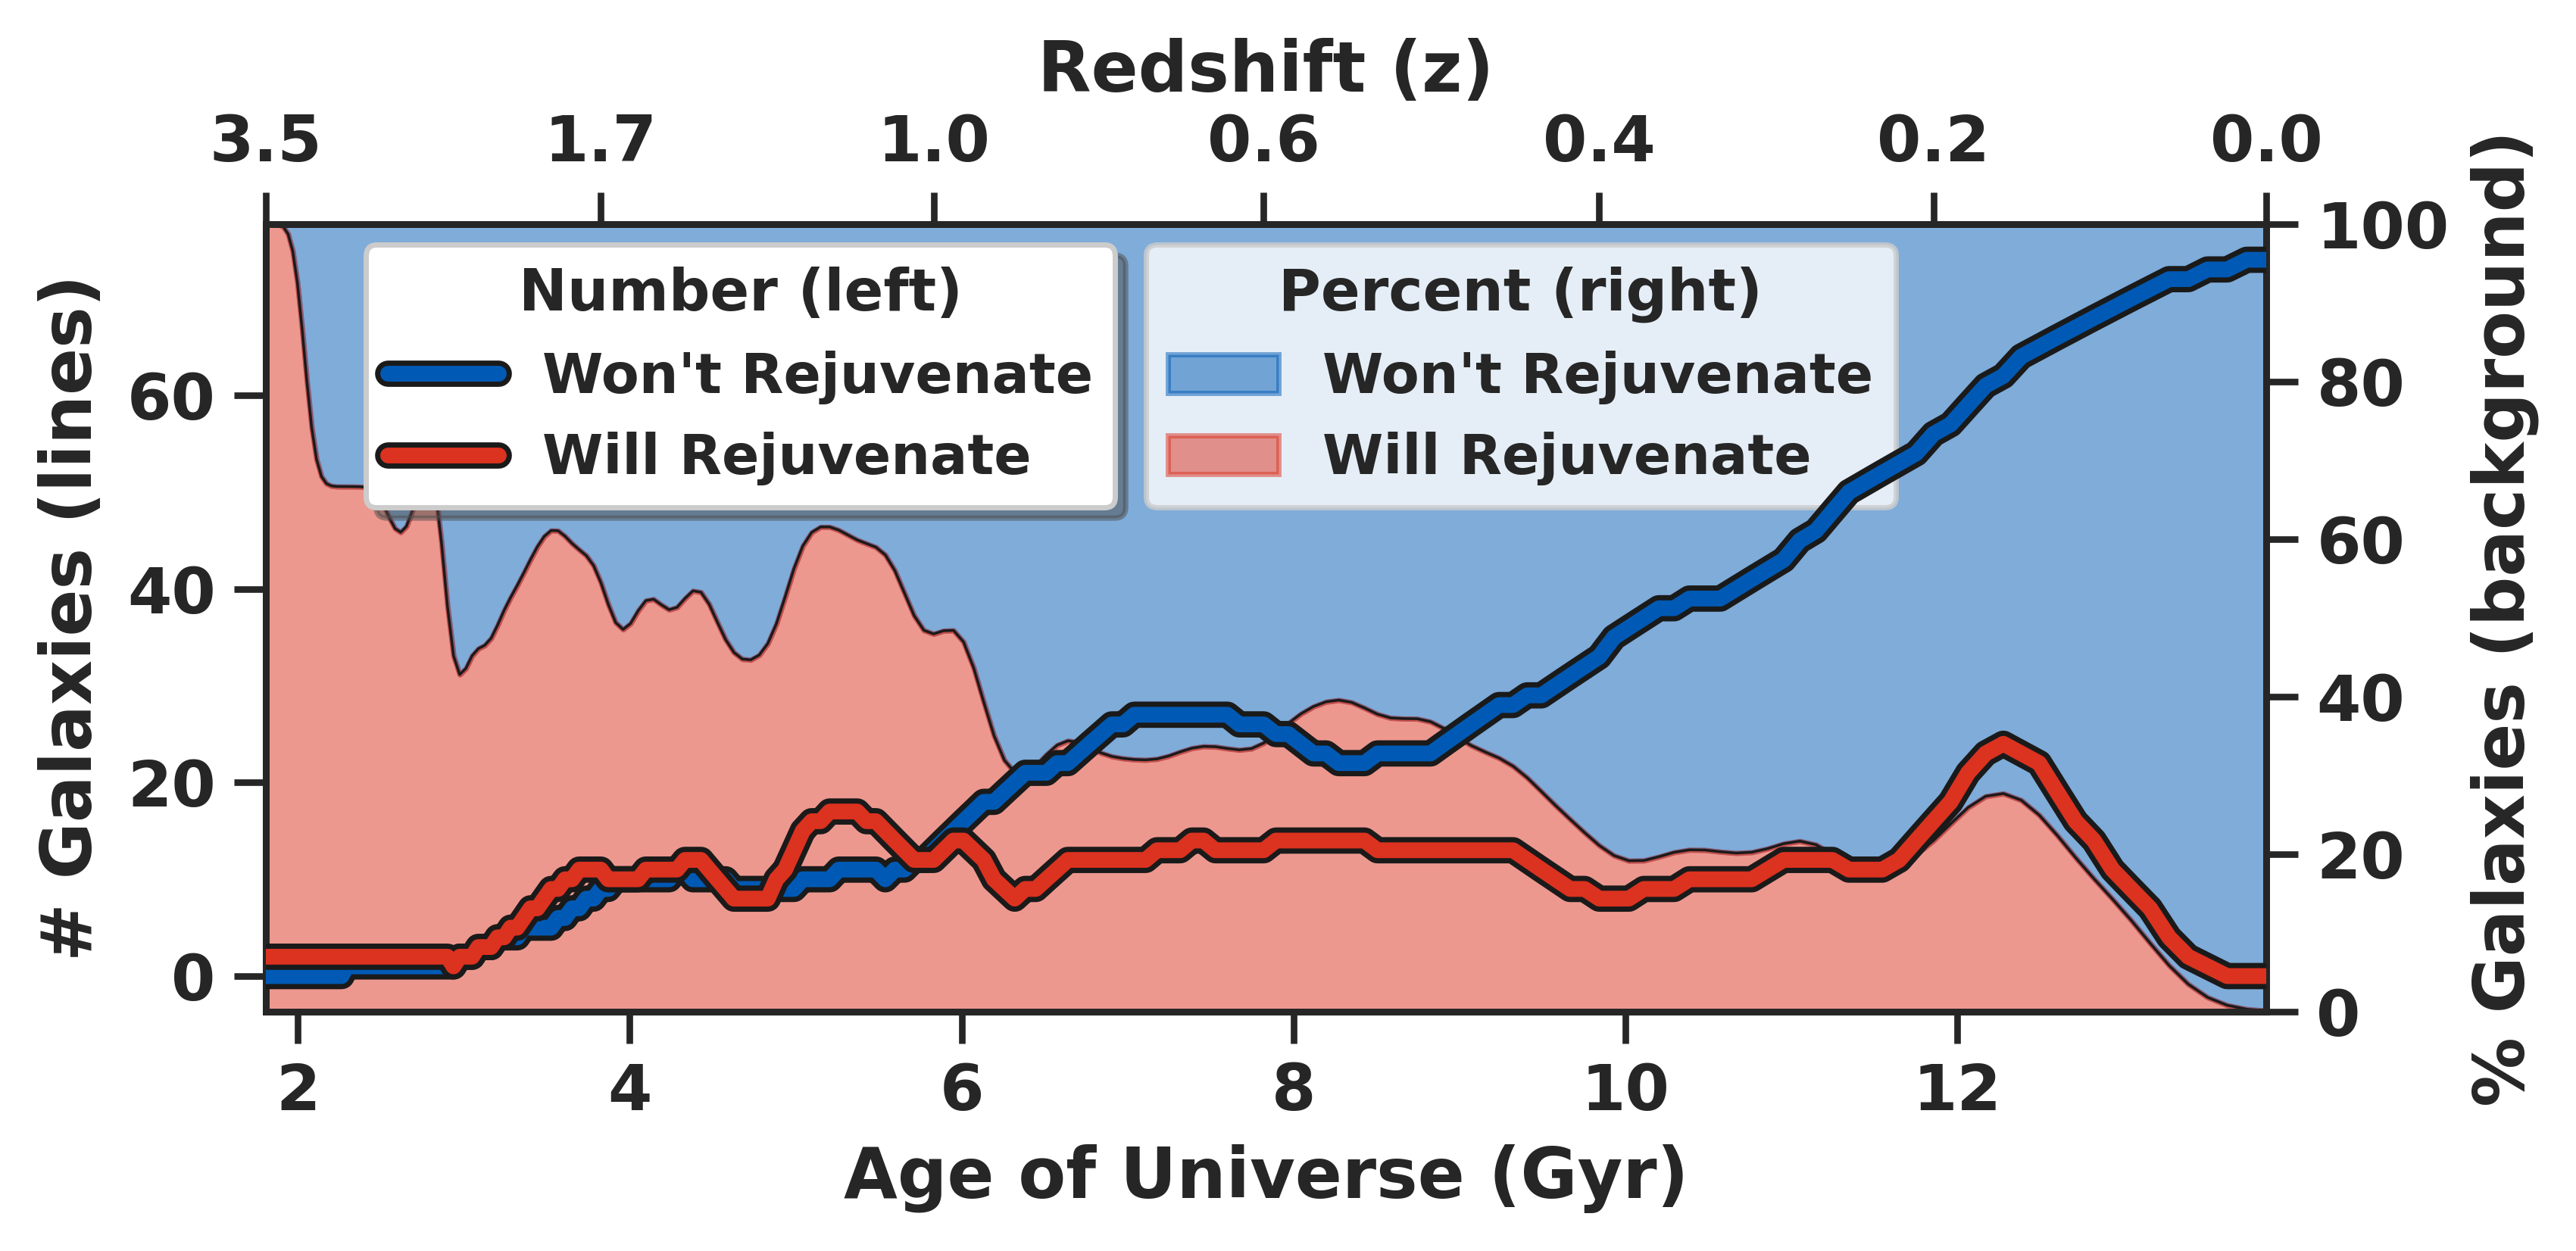
\includegraphics[width=\columnwidth]{fig2_rejuvStats_V2(2).png}
       \caption{{\bf Total number of high-mass (\eq \ref{eq:massLimit}) \textit{and} low star-forming (\eq \ref{eq:ssfrt4}) galaxies that will rejuvenate (red line) and won't rejuvenate (blue line).}  The background is shaded to represent the percent of galaxies that will (red) or won't (blue) rejuvenate, with associated values on the right $y$-axis.  We see that at high redshifts $(z>1)$, while the sample size is the smallest due to our high mass cut, as discussed in \S\ref{ssec:selectCombined}, the probability that a galaxy in our sample will rejuvenate is the highest.  In contrast, while $z=0$ provides the largest sample size for the same reason, the rejuvenation probability here is the smallest due to the rarity of galaxy interactions in the local universe.}   
    \label{fig:rejuv}
\end{figure}

To define a rejuvenation event, we loosely follow the formalism of \citet{mergers}: here, a galaxy is defined to have rejuvenated if ``after being quenched for a sufficient time, it has its sSFR return back over the star-forming cut".\footnote{Specifically, \citet{mergers} defines a rejuvenating galaxy as one that after its $\ssfr$ falls below their quenching threshold of $0.2/\tH$, it remains below $\tH^{-1}$ for at least $0.2\tH$ before having its sSFR rise back above $\tH^{-1}$}.  Applying this to our sample, we instead define a rejuvenating galaxy to be any high-mass (\eq \ref{eq:massLimit}) and initially low star-forming (\eq \ref{eq:ssfrt4}) galaxy that is able to rise back above our star-forming threshold (\eq \ref{eq:ssfrt1}; $\ssfr\times\tH=1$) for at least two consecutive snapshots.  While the exact time between snapshots depends on redshift, they are evenly spread out with respect to the logarithmic scale factor $(\log{a})$, where the scale factor is calculated as a function of redshift as $a\equiv 1/(1+z)$.  In contrast to \cite{mergers}, we soften the requirement needed for the galaxy to become eligible for rejuvenation, as our goal here is not to focus exclusively on strongly quenched galaxies, but rather to broadly quantify the likelihood of rejuvenation in any low star-forming and high-mass galaxy.

\begin{figure}
    \centering
    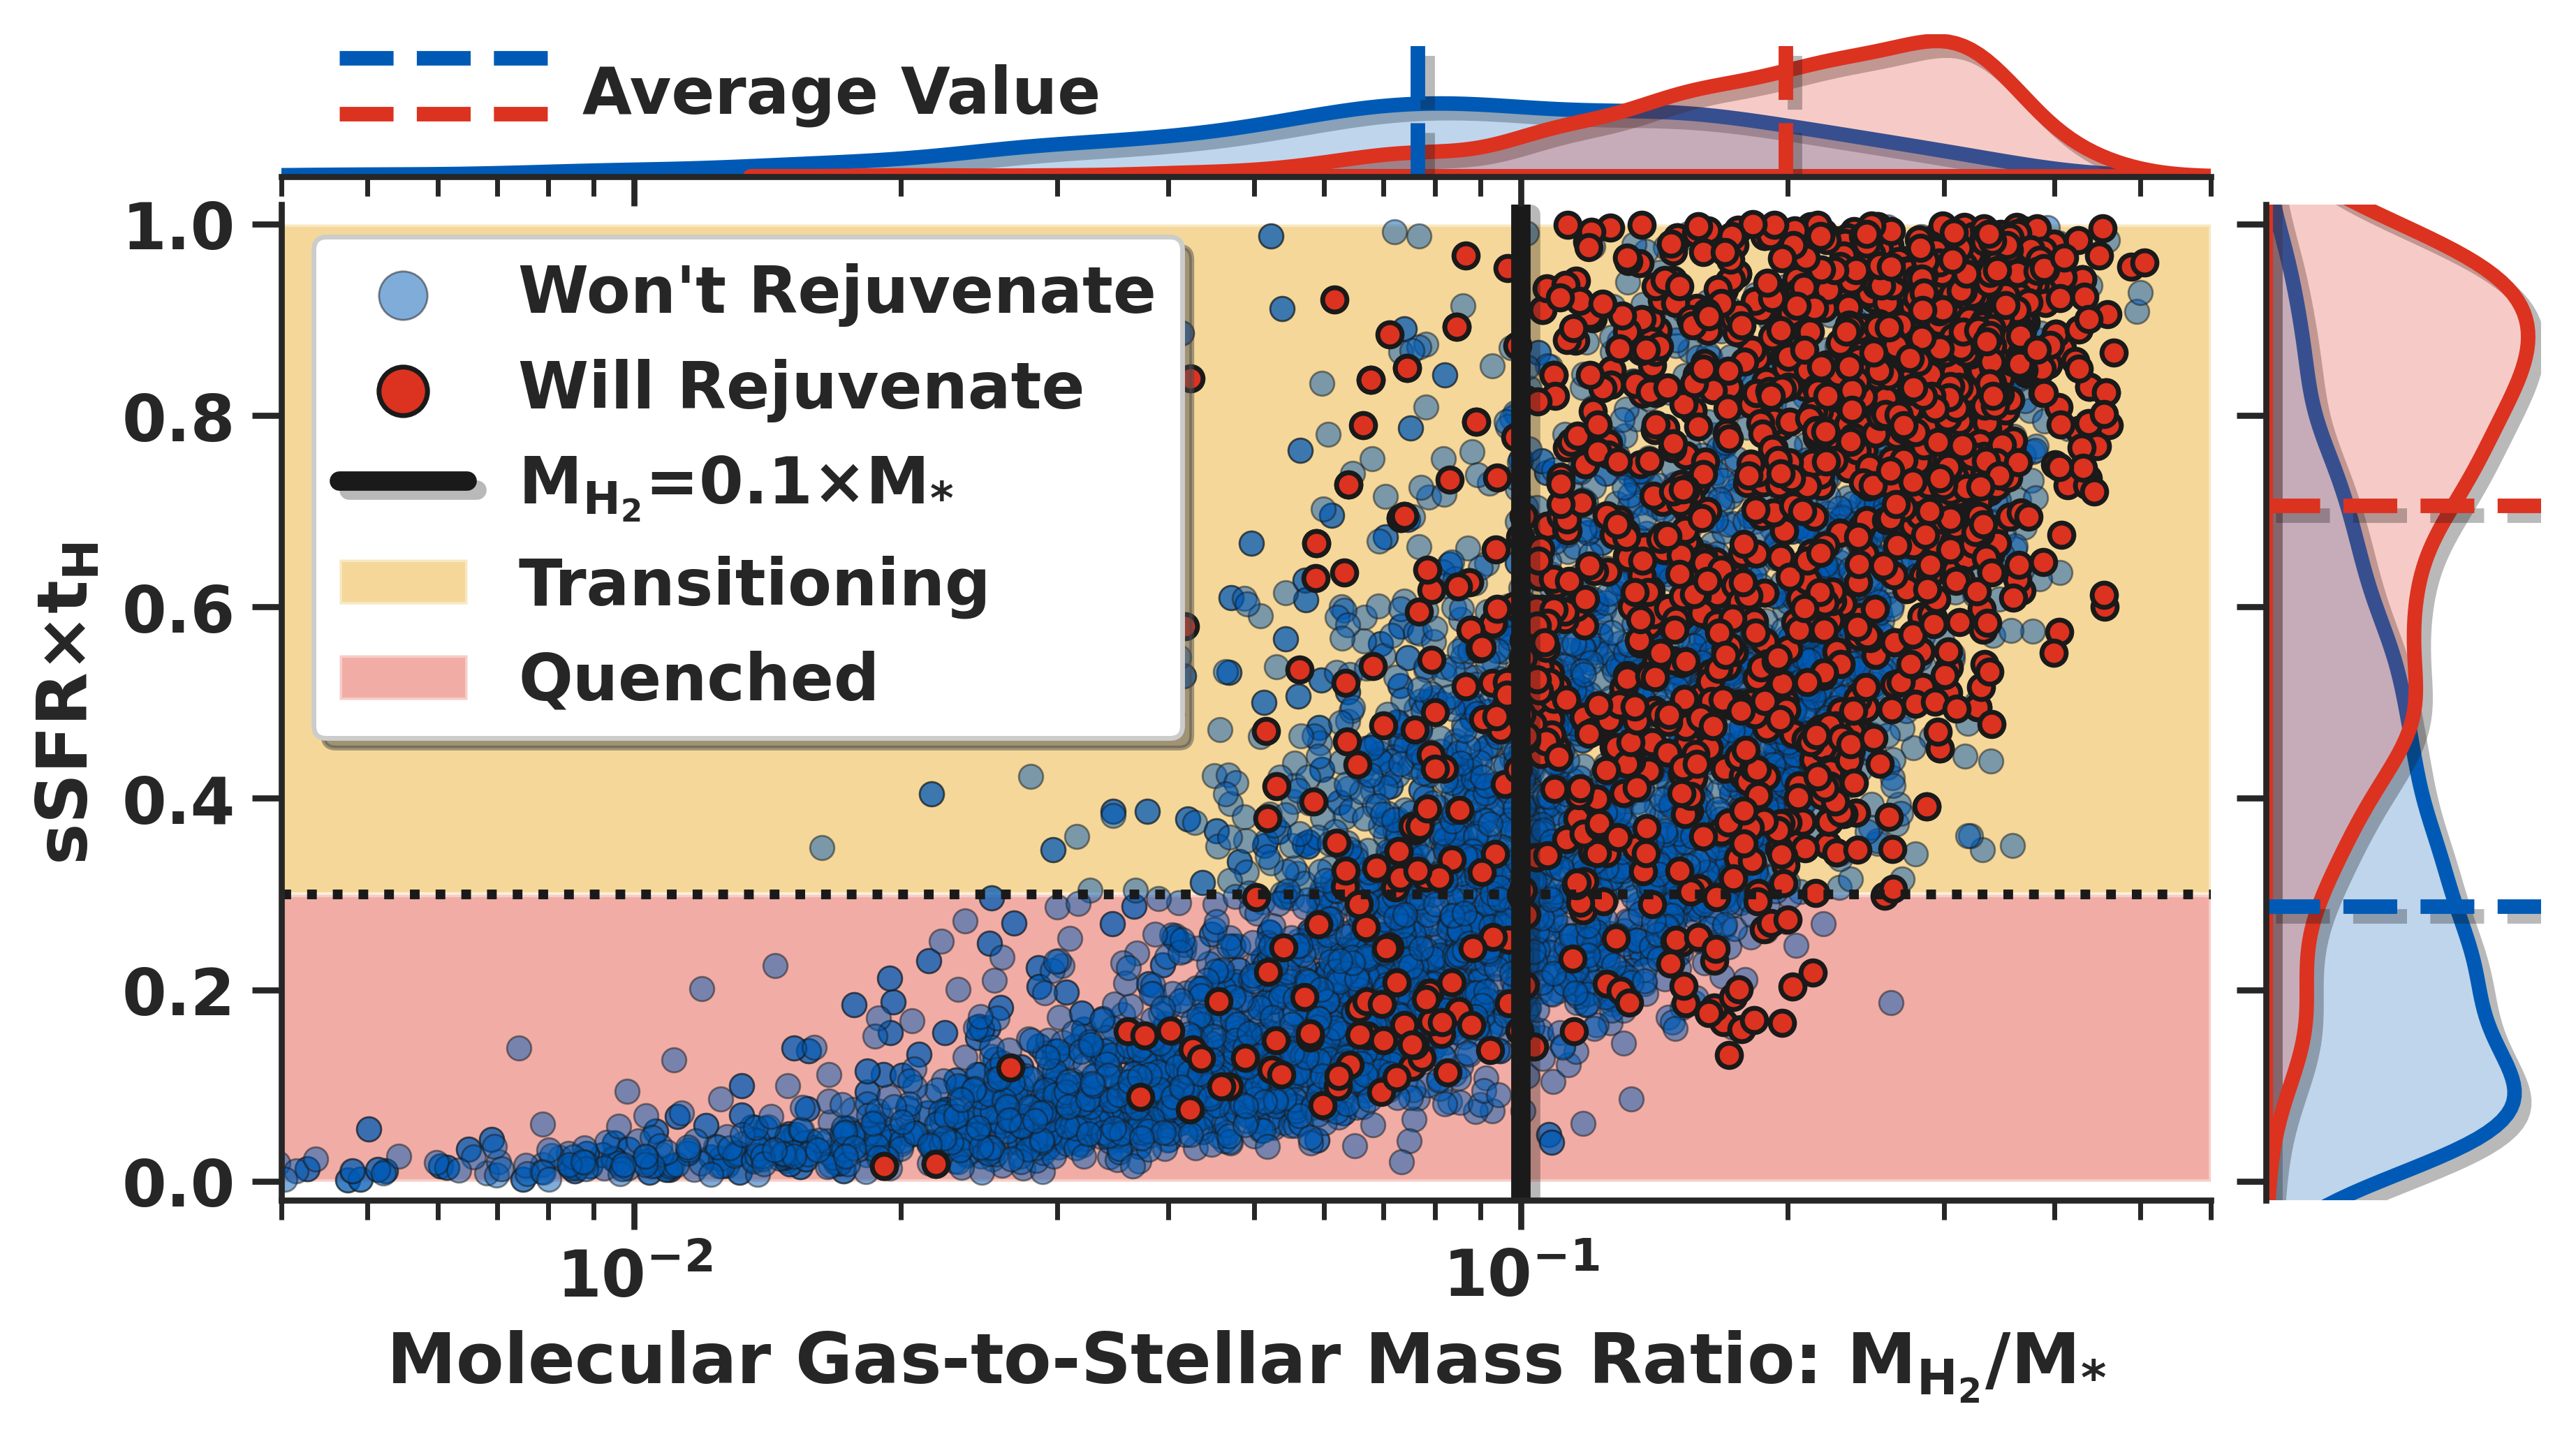
\includegraphics[width=\columnwidth]{fig3and4_rejuvJoint(2).png}
    \caption{{\textbf{Rejuvenating galaxies are significantly more star-forming and gas-rich than their non-rejuvenating counterparts for $\bm{z=0-3.5}$}}. Every point represents a galaxy from \fig \ref{fig:rejuv}, selected to be both initially low star forming and high mass (\eq \ref{eq:ssfrt4}/\ref{eq:massLimit}), colored red if it will rejuvenate and blue if not, with its molecular gas-to-stellar mass ratio shown on the $x$-axis, and its associated value of $\ssfr\times\tH$ on the $y$-axis.  On the top/right sides of the plot we also show the marginal distributions for each population as a KDE plot, with the stellar mass weighted averages shown as dotted lines.  We see from this that the majority of rejuvenating galaxies have $\mhh/M_*>0.1$ (solid black line), implying they are gas-rich, and are predominantly `transitioning' (yellow region; \eq\ref{eq:ssfrt2}), while those that will not rejuvenate are primarily quenched (red region; \eq\ref{eq:ssfrt3}) }
    \label{fig:rejuvComb}
\end{figure}
\begin{figure*}
    \centering
    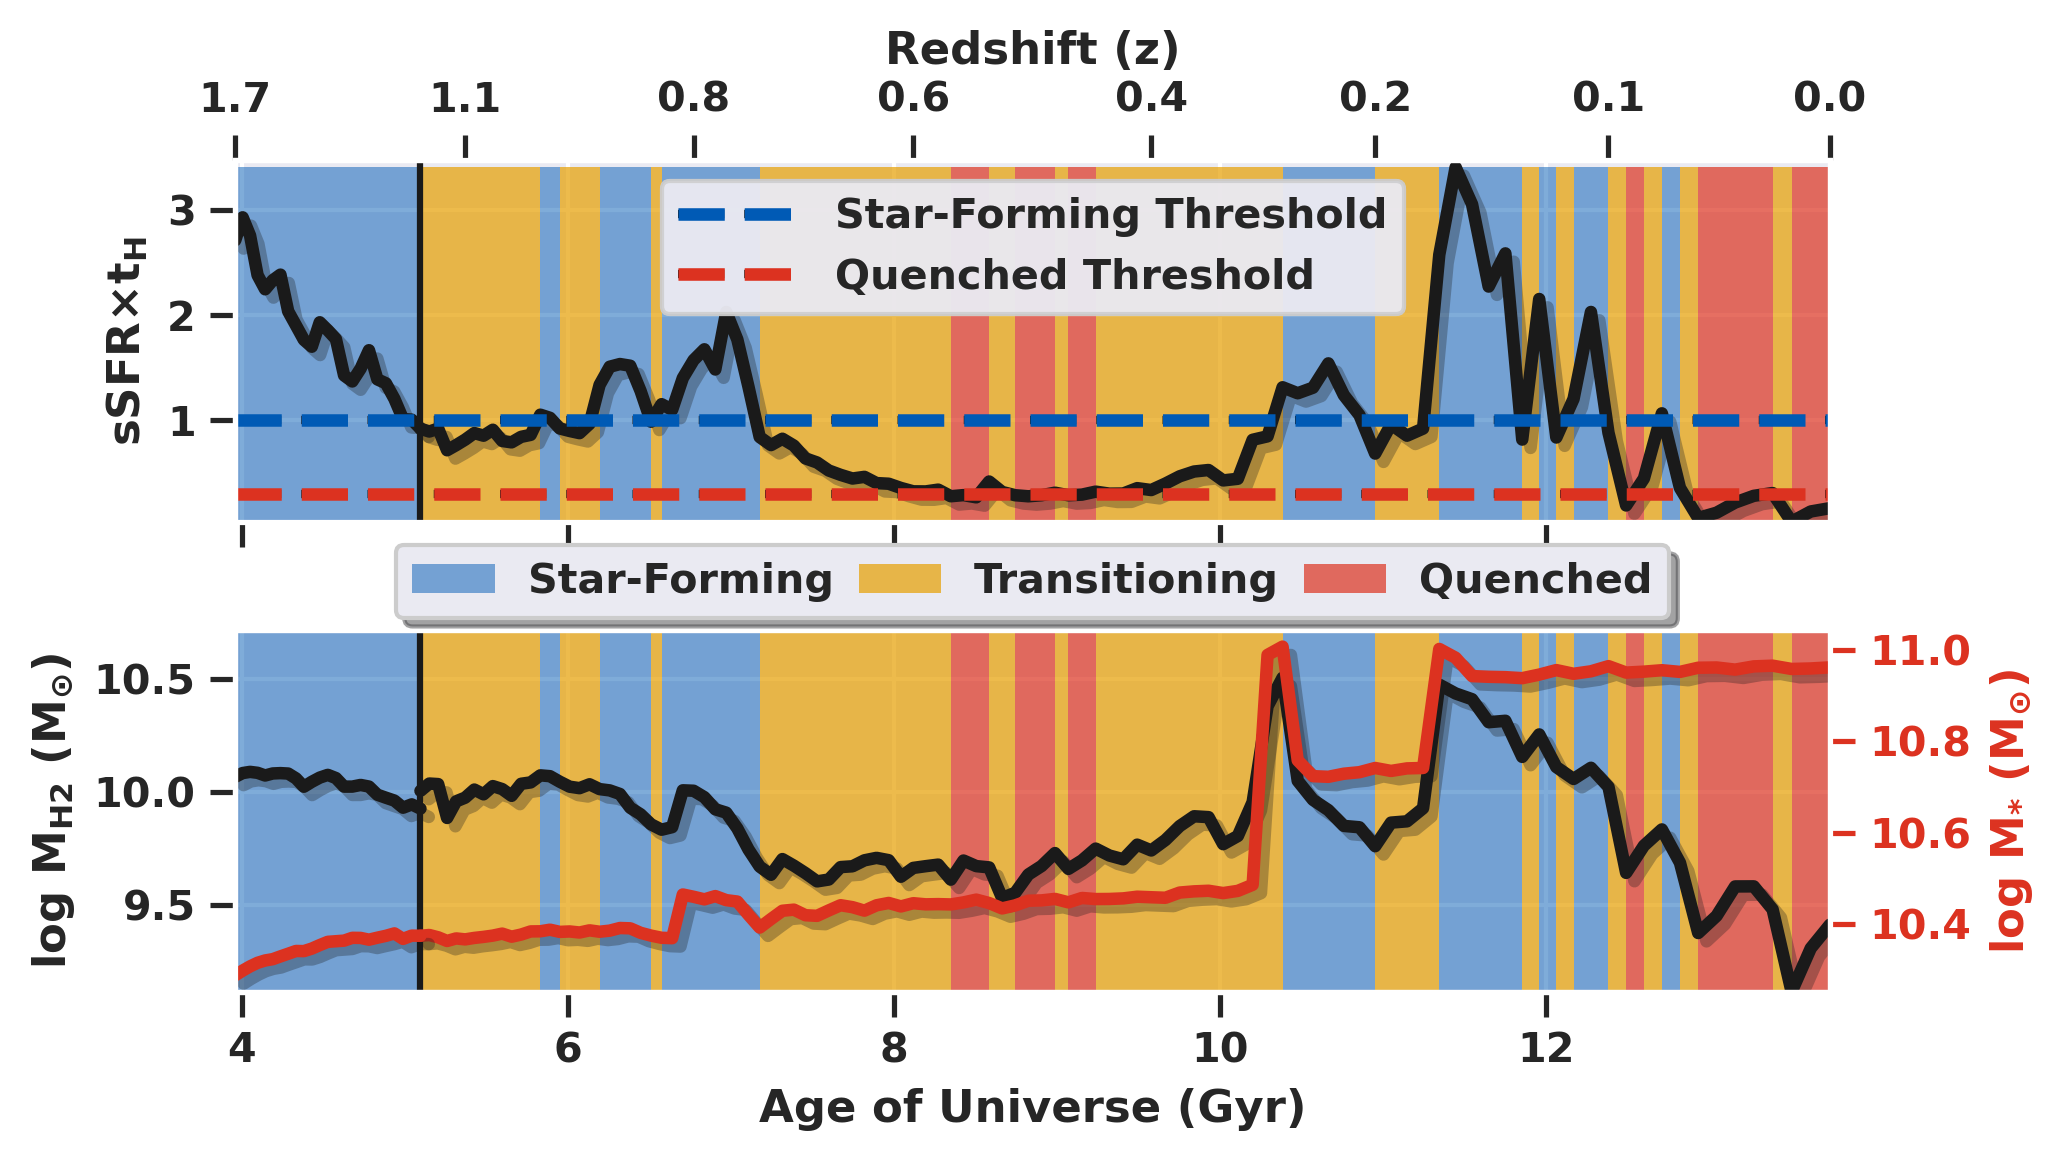
\includegraphics[width=\linewidth]{fig5_rejuvCase(2).png}
    \caption{{\bf Example of a rejuvenating galaxy}, selected at $z\approx 1.2$ (vertical black line; $\tH\sim 5.1$\,Gyr), based on it satisfying both our conditions for being low star-forming (\eq \ref{eq:ssfrt4}) and high mass (\eq \ref{eq:massLimit}), with the background color set to the star-forming classification of the galaxy based on \eq \ref{eq:ssfrt1}-\ref{eq:ssfrt3}.  While the top panel shows the evolution of $\ssfr\times \tH$, the bottom panel shows the corresponding evolution of $\hh$ mass (left/black) and stellar mass (right/red), both of which show a gradual evolution at high redshift, followed by a dramatic increase at around $z\approx 0.3$ driven by a major merging event.  The drop-off after this and subsequent rise show that the merging galaxy initially passes through our main galaxy, but, now bound within its potential well, later falls back and ultimately merges with it.  This scenario was confirmed in \app \ref{app:merge} via density projection plots.}
    \label{fig:rejuvCase}
\end{figure*}

The results of this analysis are shown in \fig \ref{fig:rejuv}, where for each redshift we show the total number (left) and percent (right) of our low star-forming and high-mass galaxies (\eq \ref{eq:ssfrt4}/\ref{eq:massLimit}) that will (red) and won't (blue) rejuvenate.  The left-hand $y$-axis indicates the total number of galaxies at each redshift that will (red line) and won't (blue line) rejuvenate, while the right-hand $y$-axis, which describes the background color, instead shows the total percent of galaxies that will (red) or won't (blue) rejuvenate.  We note that the values shown in \fig \ref{fig:rejuv} have been smoothed to aid visualization, using a 1D Gaussian ($\sigma=2$) filter from {\sc scipy.ndimage}\footnote{\url{https://docs.scipy.org/doc/scipy/reference/generated/scipy.ndimage.gaussian_filter1d.html}}, which replaces points with a weighted average of nearby points via a Gaussian kernel.

Examining \fig \ref{fig:rejuv}, we see that while rejuvenation can be an important effect at high redshift, it reduces in relative likelihood at low redshift (as also found in \citealt{Szpila25}).  To expand on this, we see that while at high redshift the occurrence of rejuvenations is the highest, the sample size is also the smallest ($N\lesssim 5$) due to the lack of high-mass galaxies at high-$z$ (as discussed in \ref{ssec:selectCombined}).  In contrast, as redshifts decrease, the amount of low star-forming and high-mass galaxies that will rejuvenate increases towards a maximum value at around $z\sim 0.2$, then falls to near zero at present day due to the rarity of galaxy interactions capable of reigniting star formation in the local universe.  At the same time, the number of such galaxies that do not rejuvenate grows at a considerably higher rate than those that do, driving the overall fraction of non-rejuvenating galaxies to approximately $100\%$ by $z=0$.  We note that while such galaxies may still rejuvenate in the future, not enough time has passed for them to have rejuvenated by the present day. 


Given the results of \fig \ref{fig:rejuv}, it becomes instructive to ask what physical differences exist between those galaxies in our sample that rejuvenated or not.  This is accomplished in \fig \ref{fig:rejuvComb}, in which we include all galaxies from \fig \ref{fig:rejuv} on a plot of molecular gas-to-stellar mass fraction vs $\ssfr\times\tH$, for all snapshots from $z=0-3.5$, colored only by whether they will (red) or won't (blue) rejuvenate.  On the top/right sides of \fig \ref{fig:rejuvComb} we show the marginal distributions for each population as a KDE plot, with the stellar-mass weighted averages shown as dotted lines.  Examining the distributions in \fig \ref{fig:rejuvComb} along the $x$-axis, we see immediately that the galaxies that will rejuvenate are much more molecular gas-rich relative to those that won't, with $\sim90\%$ of rejuvenating galaxies having $\mhh/M_*>0.1$ (solid black vertical line).  This threshold appears to mark the minimum reservoir of cold molecular gas necessary to reignite star formation within $\sim$Gyr timescales, consistent with observational studies of gas-rich quenched galaxies \citep[e.g.][]{french_2015, rowlands}.


Examining the distributions along the $y$-axis shows that rejuvenating galaxies are significantly more star forming than their non-rejuvenating counterparts for $z=0-3.5$.  The background color of the plot are shaded to represent their star-formation classification according to \S\ref{ssec:select}, where the yellow background corresponds to `transitioning' (\eq\ref{eq:ssfrt2}), while the red background is `quenched' (\eq\ref{eq:ssfrt3}).  We see that galaxies that won't rejuvenate have values of $\ssfr\times\tH$ skewed towards the smallest values, with an average value that would fall in our `quenched' category (\eq\ref{eq:ssfrt3}), implying that these systems are fully quiescent.  In contrast, $\sim 94\%$ of the rejuvenating systems lie in our `transitioning' regime (\eq\ref{eq:ssfrt2}).  Taken as a whole, \fig\ref{fig:rejuvComb} shows that the galaxies that will rejuvenate are both (a) rich in molecular gas (relative to stellar mass) and (b) are not yet fully quenched.

To probe deeper, we show the individual star formation history (SFH) for an example rejuvenating galaxy in \fig \ref{fig:rejuvCase}.  This galaxy was selected at $z\approx 1.2$ (vertical black line; $\tH\sim 5.1$\,Gyr), based on it satisfying both our conditions for being low star forming (\eq \ref{eq:ssfrt4}) and high mass (\eq \ref{eq:massLimit}), with the background color set to the star-forming classification of the galaxy based on \eq \ref{eq:ssfrt1}-\ref{eq:ssfrt3}.  The galaxy was tracked forward in time using descendant tracking, and backward to $\tH\sim 4$\, Gyr using progenitor tracking (see \S\ref{ssec:prog} for details).  The bottom panel shows the evolution of H$_2$ mass (left/black) and stellar mass (right/red), showing that this galaxy would be defined as high mass (\eq \ref{eq:massLimit}) for all points in time.  The top panel shows the corresponding evolution of $\ssfr\times\tH$ as a solid black line, showing that the periodic and often-times bursty nature of star formation can cause galaxies to fall below the star-forming threshold many times, causing multiple rejuvenation events based on our simplified definition.  A stricter criterion for rejuvenation would force galaxies to first fall below our quenching threshold (red dashed line) before they could rejuvenate, and indeed this galaxy still would satisfy this; initially being defined as fully quenched around $\tH\sim 9$ Gyr, we see it begins to reignite its star formation around a Gyr later.

Furthermore, this rejuvenation event in its star formation is seen to be associated with a dramatic increase in both the galaxy's molecular gas content and stellar mass at around 10 Gyr (bottom row of \fig \ref{fig:rejuvCase}), indicating a major gas-rich merging event occurring here. Confirmation of this scenario was achieved by examining the projection plots of our target galaxy over time, shown in \app \ref{app:merge}, in which we can visually observe the companion galaxy passing through our target system and eventually merging with it.  More details about this interaction and the associated projection plots are shown in \app \ref{app:merge}.

In summary, by examining the example rejuvenating galaxy in \fig \ref{fig:rejuvCase}, we learned that rejuvenation events can be triggered by a gas-rich major merging event.  In \fig \ref{fig:rejuvComb}, we combined our sample of high-mass and low star-forming galaxies over all $z=0-3.5$ to show that those galaxies that will rejuvenate are more gas rich and have significantly higher levels of star formation than those that do not rejuvenate.  With \fig \ref{fig:rejuv} we analyzed the redshift dependence associated with rejuvenation, and showed that the highest probability of rejuvenation occurs at high redshift.  Despite having the lowest sample size of galaxies that fit our combined selection criteria (\S\ref{ssec:selectCombined}) at high-$z$ due to the effects of our high-mass cut, as discussed in \S\ref{ssec:massLimit}, the abundance of major mergers at high-$z$ is most likely what drives the high probability of rejuvenation here.  In contrast, while the largest sample of galaxies that are both low star forming and high mass (\eq \ref{eq:ssfrt4}/\ref{eq:massLimit}) are found at low redshift, the probability of rejuvenation here is also the smallest. While such galaxies may still rejuvenate in the future, the salient point is that they have not yet had time to rejuvenate by $z=0$.

Putting it all together paints a picture in which among the low star-forming and high-mass (\eq \ref{eq:ssfrt4}/\ref{eq:massLimit}) galaxies, those that will rejuvenate are those that are relatively molecular ($\hh$) gas rich and have not yet fully quenched.  While these findings could explain why galaxies with persistent molecular gas reservoirs could appear to have anomalously low SFRs, such as those from \cite{suessSquiggle} ($0.5<z\leq 0.9$), it does not resolve the question of why their molecular gas seems to disappear on extremely fast ($\sim150$ Myr) timescales \citep{setton2025}.

%===== Hypothesis #2 =====
\subsection{Hypothesis B: Incorrect Alpha-CO}
\label{ssec:HD}
\begin{figure*}[hbt!]
   \centering
    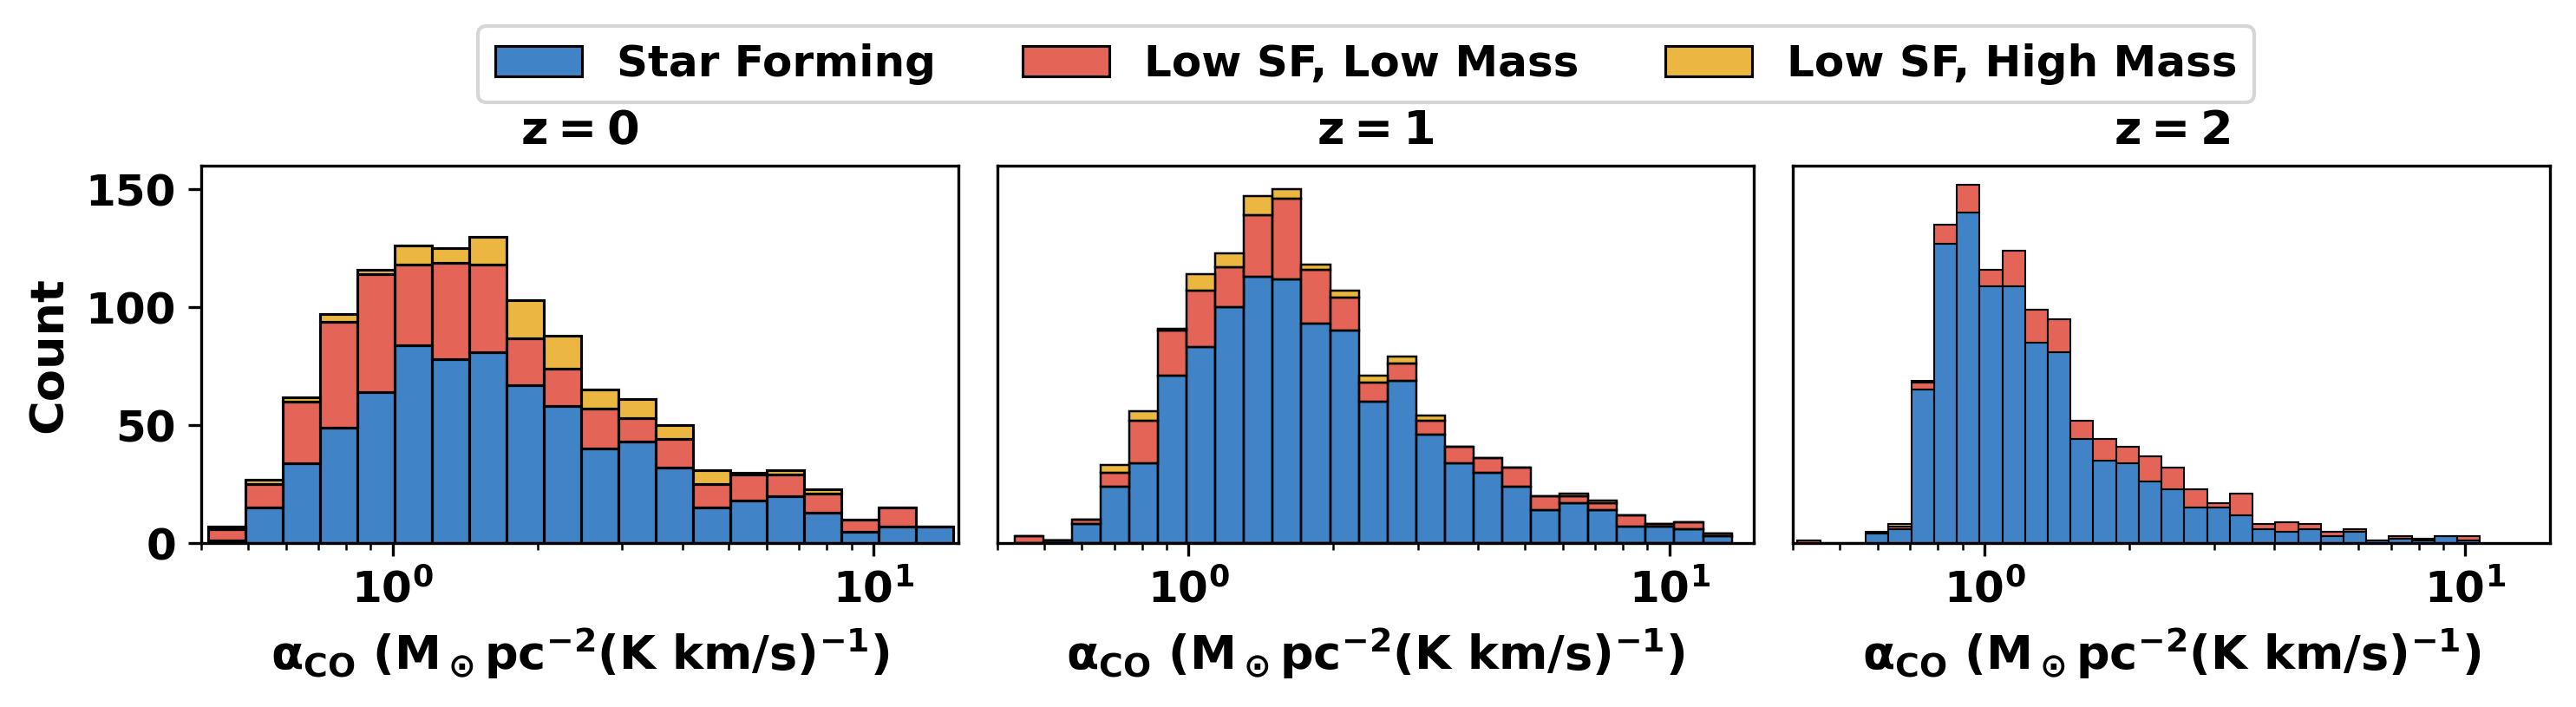
\includegraphics[width=\linewidth]{fig6_alphaCO.png}
    \caption{{\bf All galaxies have similar $\bm{\aco}$ distributions, regardless of mass or star formation level, which decrease towards higher redshifts.} For each $\aco$ bin, the bars show the number of galaxies categorized as star forming (\eq \ref{eq:ssfrt1}) in blue, low star forming and low mass (\eq \ref{eq:ssfrt4}/\ref{eq:massLowLim}) in red, and those that satisfy our combined selection criteria (\S\ref{ssec:selectCombined}) of being both low star forming and high mass (\eq \ref{eq:ssfrt4}/\ref{eq:massLimit}) in yellow.  Due to the effects of restricting our sample to high mass, as discussed in \S\ref{ssec:massLimit}, the number of galaxies that fit our combined selection criteria (yellow bars) drops to near-zero at $z=2$.  Since most systems have $\aco<\acomw$, an observer who assumes that $\aco=\acomw$ in these galaxies would infer more molecular hydrogen to be present.  Although, since the values of $\aco$ tend to lie co-spatially on the histograms (regardless of star formation or mass levels), we conclude that this hypothesis cannot explain why we see molecular gas specifically present in massive quenched galaxies, but instead suggests a fundamental shift that must be applied to all scaling relations.}
    \label{fig:alphaCO}
\end{figure*}
Our second hypothesis explores whether an incorrectly assumed value of the CO-to-H$_2$ conversion factor ($\alpha_\text{CO}$) could be the root cause of the seemingly abundant molecular gas reservoirs observed in massive quenched galaxies.  Since $\hh$ resides primarily in cool giant molecular clouds \citep[GMCs;][]{Mckee07}, yet only emits directly at high temperatures, it is nearly invisible via direct emission in these environments and thus must be traced using the next most abundant molecule, carbon monoxide (CO).  After measuring the velocity-integrated CO luminosity in a GMC $(L_{\text{CO}}')$, the corresponding molecular gas mass $(\mgas)$ can be estimated by using the CO-to-H$_2$ conversion factor ($\aco$), defined as $\aco=\mgas/L_{\text{CO}}'$ \citep{Bolatto_2013, alphaCO}.  Owing to the large number of studies of this factor in the Milky Way that converge on a characteristic value of $\acomw=4.4\ \text{M}_\odot \text{pc}^{-2} (\text{K}~\text{km/s})^{-1}$ \citep{Narayanan2013,Bolatto_2013}, extragalactic studies often adopt this Milky Way value for $\aco$ across all galaxies.

Since systematic variations of $\aco$ with various ISM properties are both expected and observed \citep{Strong04,narayanan12, Sandstrom13}, in this section we will explore how the common assumption that $\aco=\acomw$ will impact the inferred molecular gas in massive gas-rich quiescent galaxies.  All values needed to calculate $\aco=\mgas/L_{\text{CO}}'$ are computed in post-processing using the \slick code \citep{slick}, which derives model CO luminosities by splitting up each gas particle into concentric radial zones \citep{popping} and computing thermal, radiative, and statistical equilibrium throughout the sub-grid model using \despotic\!\!\footnote{\despotic is a code to Derive the Energetics and SPectra of Optically Thick interstellar Clouds and can be found at \url{https://bitbucket.org/krumholz/despotic/src/master/}.}\citep{despotic}.  In this formalism, each gas particle can be thought of as representing a giant molecular cloud (GMC).  

The molecular gas $(\mgas)$ in our model assumes a GMC composition of molecular Hydrogen (H$_2$) and atomic Helium (He), in which the Helium mass is 40\% of H$_2$, so that $\mgas \equiv \mhh+M_{\text{H}_e}=\mhh(1+0.4)=7\mhh/5$.  Then to calculate $\aco$ for a galaxy in our simulation, we computed the total molecular gas mass of each gas particle that converged in post-processing, add their velocity-integrated CO luminosities, and obtain their ratio to get $\aco$.  All values from \slick and methods used to calculate $\aco$ were supplied by D. Valentin-Martinez (private), who is exploring $\aco$ throughout cosmic time (D. Valentin-Martinez et al., 2026, in preparation).

To visualize the distribution of $\aco$ calculated for our galaxies, we show a histogram of their $\aco$ in \fig \ref{fig:alphaCO}.  The bars are separated into those that are star forming (\eq \ref{eq:ssfrt1}) in blue, those that are low star forming (\eq \ref{eq:ssfrt4}) and low mass (\eq \ref{eq:massLowLim}) in red, and those that satisfy our combined selection criteria (\S\ref{ssec:selectCombined}) of being both low star forming (\eq \ref{eq:ssfrt4}) and high mass (\eq \ref{eq:massLimit}) in yellow.  Given that the standard value of $\aco$ derived in our Milky-Way is $\acomw=4.4\ \text{M}_\odot \text{pc}^{-2} (\text{K}~\text{km/s})^{-1}$ \citep{Bolatto_2013}, we show in \fig\ref{fig:alphaCO} that while at $z=0$ approximately 2/3 of our galaxies have $\aco<\acomw$, this increases to $\sim$100\% at higher redshifts.

The upshot of Figure~\ref{fig:alphaCO} is that the $\aco$\ values between different galaxy populations are indistinguishable in our model.  Since $\aco$ does not vary systematically based on mass or star formation classification, we conclude that this hypothesis is not likely to answer why we see an abundance of molecular gas in massive quenched galaxies (as also found by \citealt{setton2025}).

%===== Hypothesis #3 =====
\subsection{Hypothesis C: Dust Obscuration}
\label{ssec:HC}
Our third hypothesis is that massive galaxies that appear to be quenched, but are rich in molecular gas, are actually harboring dust-obscured star formation, and are not actually quenched at all \citep[e.g.,][]{Baron22, Baron2023, pengPei, cenci25}.  Specifically, \cite{Baron2023} analyzed NOEMA CO(1-0) observations of 15 post-starburst galaxies with a multiwavelength approach, finding that while some regions of the galaxy are indeed quenched, other parts of the galaxy are instead forming stars in highly obscured regions.

In contrast to the previous two hypotheses, in this section we instead select our sample of galaxies based on their colors instead of their SFR, as we are testing whether or not star-forming galaxies can mimic signatures of quenched galaxies in their observational spectra (in other words: in order to fully test this hypothesis, we need to select low star-forming galaxies in a manner similar to observers).  To generate realistic mock spectral energy distributions (SEDs) for our sample of galaxies, we post-process our simulated snapshots using the dust radiative transfer code \powderday (\url{https://github.com/dnarayanan/powderday}).  First introduced in \cite{powderday}, \powderday uses \fsps for stellar population synthesis models \citep{conroy1, conroy2, conroy3}, \hyperion for radiative transfer \citep{hyperion}, and \yt to interface between varying software packages \citep{yt}.

When running \powderday to produce mock SEDs, we first smooth the particle data onto an octree to setup the model for radiative transfer.  Next, we employ \fsps to generate a simple stellar population (SSP) for each star particle.  For consistency with \simba\!\!\!, we use a Chabrier initial mass function (IMF) \citep{simba}.  Combined with MIST isochrones \citep{Choi16, Dotter_2016} and a MILES stellar spectral library \citep{Sanchez06} as our fiducial SPS parameters, we then run \fsps to create a dust-free stellar SED.  Given the initial stellar SED from \fsps and the grid from \yt\!\!, \hyperion is then employed to run 3D radiative transfer via a Monte Carlo algorithm to produce the final SED \citep{hyperion}.  Finally, the resulting SED is extracted by assuming the largest aperture size available to the model.

To select our sample of galaxies, we follow the method in \cite{suessSquiggle}, which uses synthetic medium-band rest-frame filters ($U_m$, $B_m$, and $V_m)$ to define ``post-starburst galaxies" as having $U_m-B_m>0.975$ and $-0.25<B_m-V_m<0.45$ (\eq\ref{eq:UBVSelect}).  According to \cite{suessSquiggle}, the $U_m-B_m$ color is able to separate PSBs from unobscured star-forming galaxies by quantifying the strength of the Balmer break, while the $B_m-V_m$ color is able to separate PSBs from dusty star-forming galaxies and older quiescent galaxies by quantifying the slope of the spectra redwards of the break. These criteria are only satisfied by a small fraction of galaxies; for example \cite{suessSquiggle} showed that for $z>0.5$, only around $\sim 5\%$ of SDSS galaxies satisfy both of these color cuts.  In our sample, we find $\sim17\%$ of galaxies at $z=0.5$ satisfy these criteria, giving a final sample of 409 UBV-selected galaxies.  A detailed comparison between these galaxies and those presented in \cite{suessSquiggle} is provided in \app \ref{app:ubv}.

\begin{figure}
    \centering
    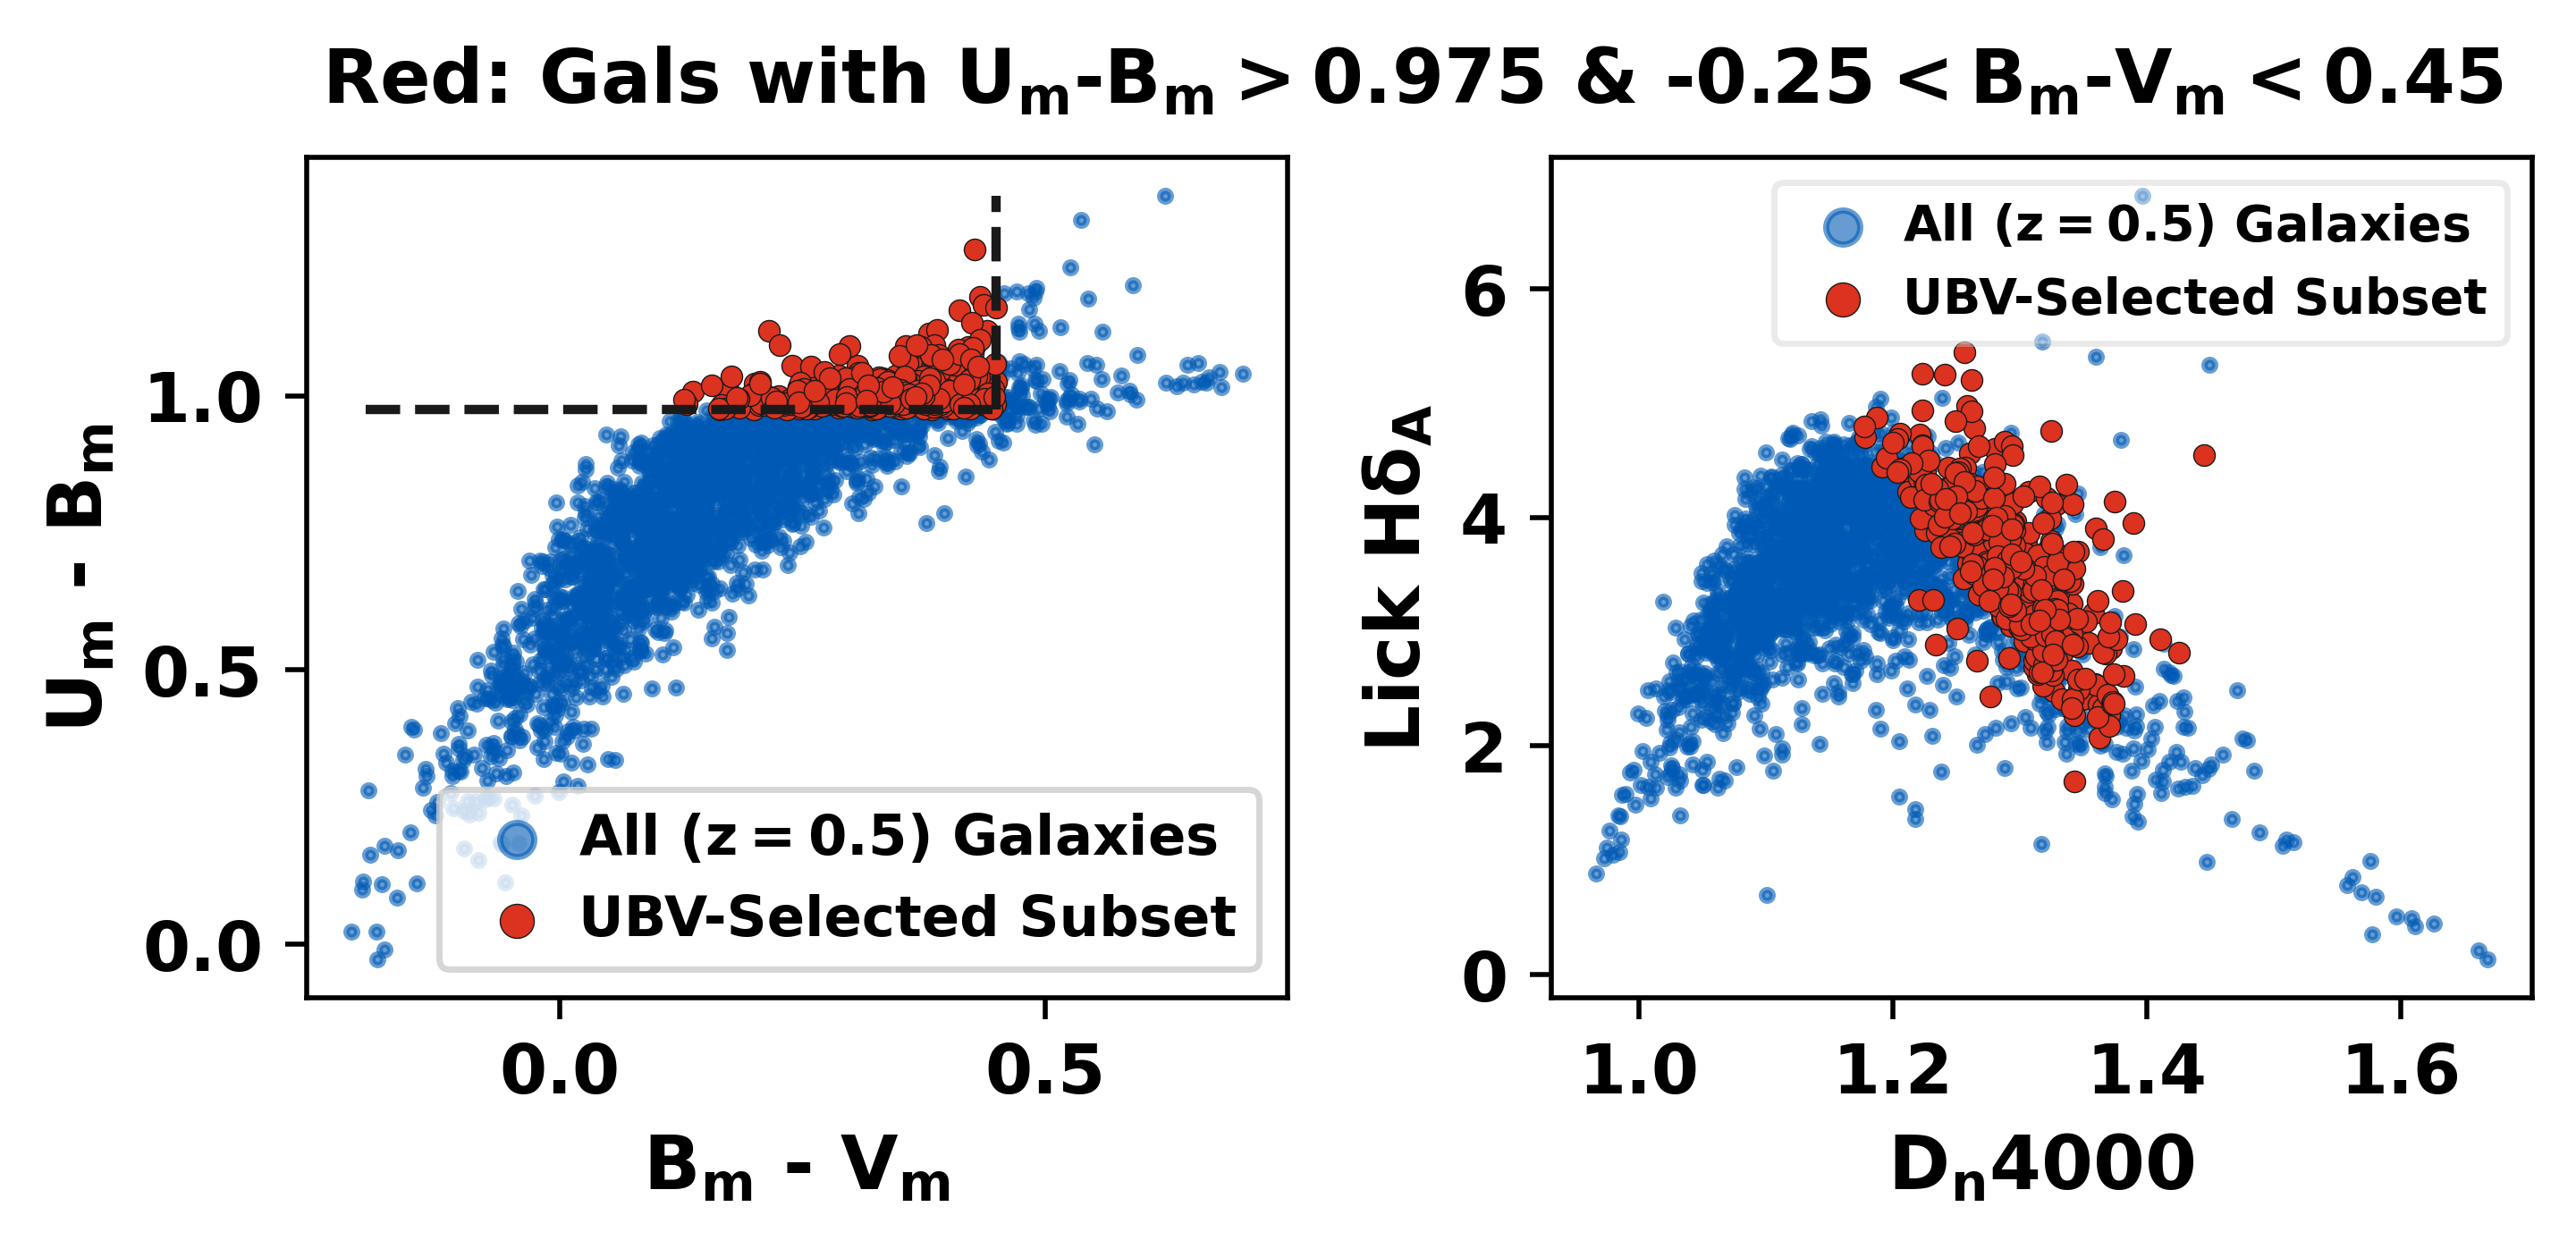
\includegraphics[width=\linewidth]{fig6_ubvSpace_z0p5(1).png}
    \caption{{\bf The distribution of our {\bfseries \scshape simba} galaxies at $\bm{z=0.5}$ in UBV space (left), and in a plot of D$\bm{_n}$4000 vs H$\bm{\delta_A}$ (right).}  The red-colored points are those that satisfy the PSB-like UBV selection from \cite{suessSquiggle}, defined to identify relatively dust-free galaxies that recently quenched after a large starburst.  The left-hand plot shows the galaxies in UBV-space, defined by the medium-band rest-frame filters ($U_m$, $B_m$, and $V_m)$, designed to target the Balmer break and slope of the spectrum redward of the break \citep{suessSquiggle}. Right-hand plot shows the galaxies lick H$\delta_A$ index (i.e. H$\delta$ EW; which traces recent star formation) as a function of the 4000\r{A} break index (which probes the age of the stellar population), such that age increases toward the lower right.}
    %  The red-colored dots correspond to galaxies that satisfy our PSB-like UBV classification of $U_m-B_m>0.975$ and $-0.25<B_m-V_m<0.45$.
    \label{fig:UBV}
\end{figure}
\begin{figure*}
    \centering
    
\includegraphics[width=\linewidth]{fig7_sfr_IR_FUV_z0p5.png}
    \caption{{\bf UBV-selected massive and molecular gas-rich (high mass; \eq\ref{eq:massLimit}) galaxies at $\bm{z=0.5}$ have an IR-based SFR that accurately traces their true SFR, yet a FUV-based SFR that significantly underestimates it.}  The left plot shows that among the UBV-selected galaxies, those that are also high mass (\eq \ref{eq:massLimit};\,\,red stars) will have an excess of dust-obscured star formation, which shifts the emitted UV starlight into the IR.  As a result, the IR luminosity traces the SFR in these systems (middle plot), while the UV luminosity severely underestimates it (right plot).}
   \label{fig:IR_FUV}
\end{figure*}

Applying this selection criterion to our sample of galaxies at $z=0.5$ produces the population colored red in \fig \ref{fig:UBV}.  The left-hand panel shows all of our galaxies in UBV-space as individual points, while the red colored dots are those galaxies that satisfy the `PSB-like' UBV selection criteria.  The right-hand plot of \fig \ref{fig:UBV} shows the same sample using alternative definitions; namely the 4000\r{A} break (D$_n$4000) and Lick index (H$\delta_A$).  The 4000\r{A} break, commonly called the D$_n$4000 index, is used largely to determine a galaxies' current state of star formation \citep{dn4000}, and is defined as the ratio between the average flux density (in erg$~$s$^{-1}$cm$^{-2}$Hz$^{-1}$) between 4000-4100\r{A} and  3850-3950\r{A}. 

In contrast, H$\delta_A$ is a Lick index developed as a standardized measure of the equivalent width of the Balmer H$\delta$ absorption line \citep{hdelta}, which is strongest for galaxies with stellar populations dominated by A-type stars, and is usually interpreted as evidence of a burst of star formation that ended 0.5-1.5 Gyr prior to observation. To calculate this, a pseudo-continuum is defined by calculating the average flux density bluewards of the line (4017\r{A}-4057\r{A}) and redwards of the line (4153\r{A}-4193\r{A}), fitting a straight line between both, then using that to integrate over the absorption line (defined between wavelengths 4083.5\r{A} and 4122.25\r{A}).  The subscript ``A" is used to define a wider bandpass, around 40\r{A}, which is more suited for measuring absorption in A-star dominated systems with intrinsically broader absorption \citep{hdelta}.

The next step in investigating this hypothesis is to take the sample of galaxies that satisfy our UBV cut (red points in \fig \ref{fig:UBV}) and investigate how the SFR derived from the IR deviates from the SFR derived from the FUV, as well as how both compare to the true SFR.  Since most SFR indicators are derived from rest-UV or optical measurements, these methods are likely to yield lower SFR estimates than expected in dust-rich systems, as a significant portion of the high-energy radiation from the galaxy is absorbed by dust and re-emitted in the infrared.  To test this hypothesis, we take our sample of UBV-selected galaxies (red points in \fig \ref{fig:UBV}) and calculate the SFR of these galaxies derived from their mock IR and far-UV photometry, to compare with the true SFR of the galaxies, with corresponding results shown in \fig \ref{fig:IR_FUV}.

Following \cite{murphy}, we define L$_{\text{IR}}$ as the integrated luminosity of our dust-attenuated SED from 8-1000$\mu$m, and convert it to an IR-based star-formation rate using $\sfr_{\text{IR}}/(\text{M}_\odot/\text{yr})=3.88\times 10^{-44}\text{L}_{\text{IR}}/(\text{erg/s})$.  Similarly, we define L$_{\text{FUV}}$ by convolving the SED with a {\sc GALEX\,\,}FUV transmission curve, and compute the corresponding FUV-based star-formation rate as $\sfr_{\text{FUV}}/(\text{M}_\odot/\text{yr})=4.42\times 10^{-44}\text{L}_{\text{FUV}}/\text{(erg/s)}$.

The results of applying this analysis to our sample of UBV-selected galaxies at $z=0.5$ are shown in \fig \ref{fig:IR_FUV}.  Here, we separate all UBV-selected selected systems by whether they satisfy our high-mass cut (red stars; \eq\ref{eq:massLimit}) or not (red dots; \eq\ref{eq:massLowLim}).  As a reminder, in \S\ref{ssec:massLimit} we defined high-mass galaxies (red stars; \eq\ref{eq:massLimit}) as any that are both massive $(M_*>10^{10}M_\odot)$ with enough molecular gas to be detectable $(\mhh>10^9 M_\odot)$, and low-mass galaxies to be any that do not satisfy this (\eq \ref{eq:massLowLim}).  In \fig \ref{fig:IR_FUV}, the left-most panel shows a direct comparison of FUV-based SFR vs IR-based SFR, showing an excess of dust-obscured star formation for high-mass galaxies.  The middle plot shows the IR-based SFR vs true SFR, and demonstrates that the high-mass galaxies (\eq \ref{eq:massLimit}) have IR luminosities that accurately trace their true SFRs, while the IR luminosity of gas-poor galaxies (\eq \ref{eq:massLowLim}) underestimates the true SFR.  Finally, the right-most plot shows FUV-based SFR vs true SFR, and shows that the UV luminosity severely underestimates the true SFR for all UBV-selected systems.

\begin{figure}
    \centering
    % \vspace*{-.1in}
     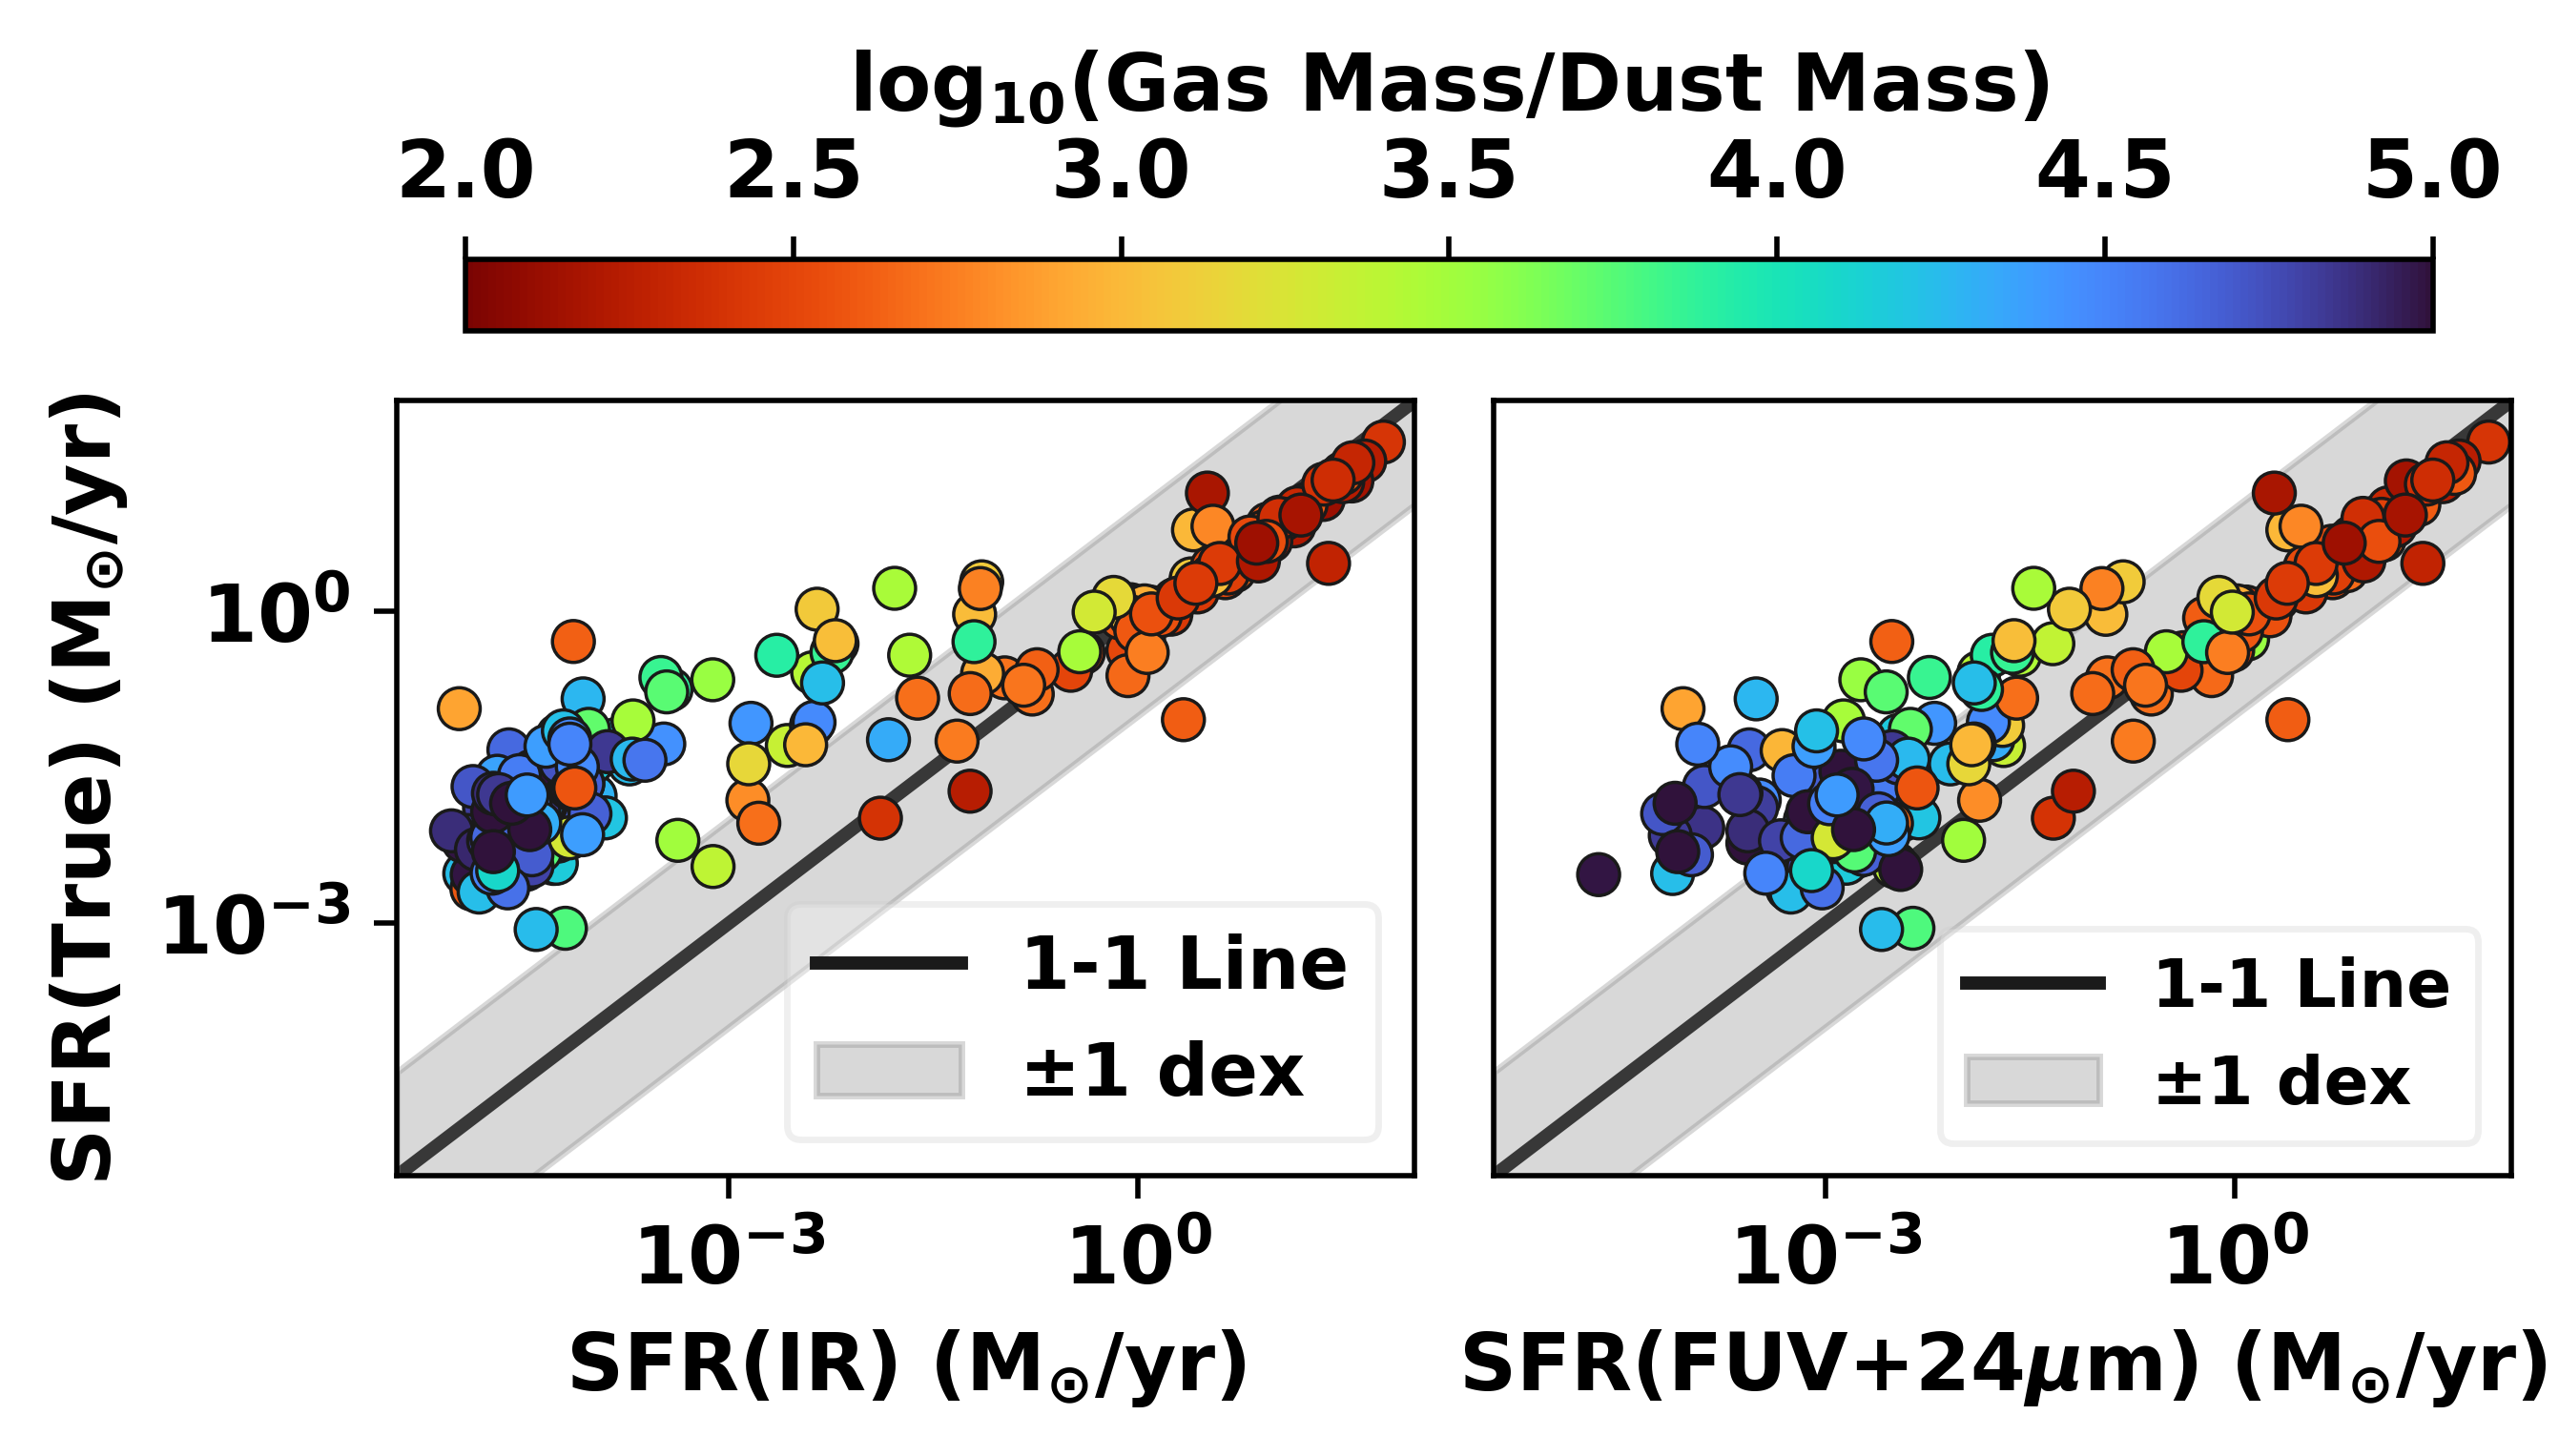
\includegraphics[width=\linewidth]{fig8_sfrIR_FUV_GD_GoldStandard_z0p5.png}
    \caption{{\bf (\underline{Left}) IR luminosity only works as a SFR diagnostic for very low (MW-like) values of the gas-to-dust ratio (GDR)}  This is the same middle panel of \fig \ref{fig:IR_FUV}, but now colored by the log ratio of the total gas-to-dust mass in each galaxy, with the value indicated by the colorbar on the top of the figure.  We see that the points on the one-to-one (black) line have low GDRs, indicating sufficient dust to reprocess UV light into IR emission, while points above the line have higher GDRs, implying dust-poor galaxies where UV escapes and IR-based SFRs are underestimated.  {\bf (\underline{Right}) the mixed FUV+24$\bm{\mu}$m SFR measurement works for all but the very high GDR values.}  While a FUV-based SFR underestimates the true SFR in all UBV-selected systems (right-most panel of \fig \ref{fig:IR_FUV}), a more holistic mixed SFR indicator \citep{Calzetti07} is shown to trace the true SFR in all systems except those with the highest GDR (i.e. dust-poor).
   }
    \label{fig:IR_FUV_GDR}
\end{figure}

\begin{figure*}
    \centering
    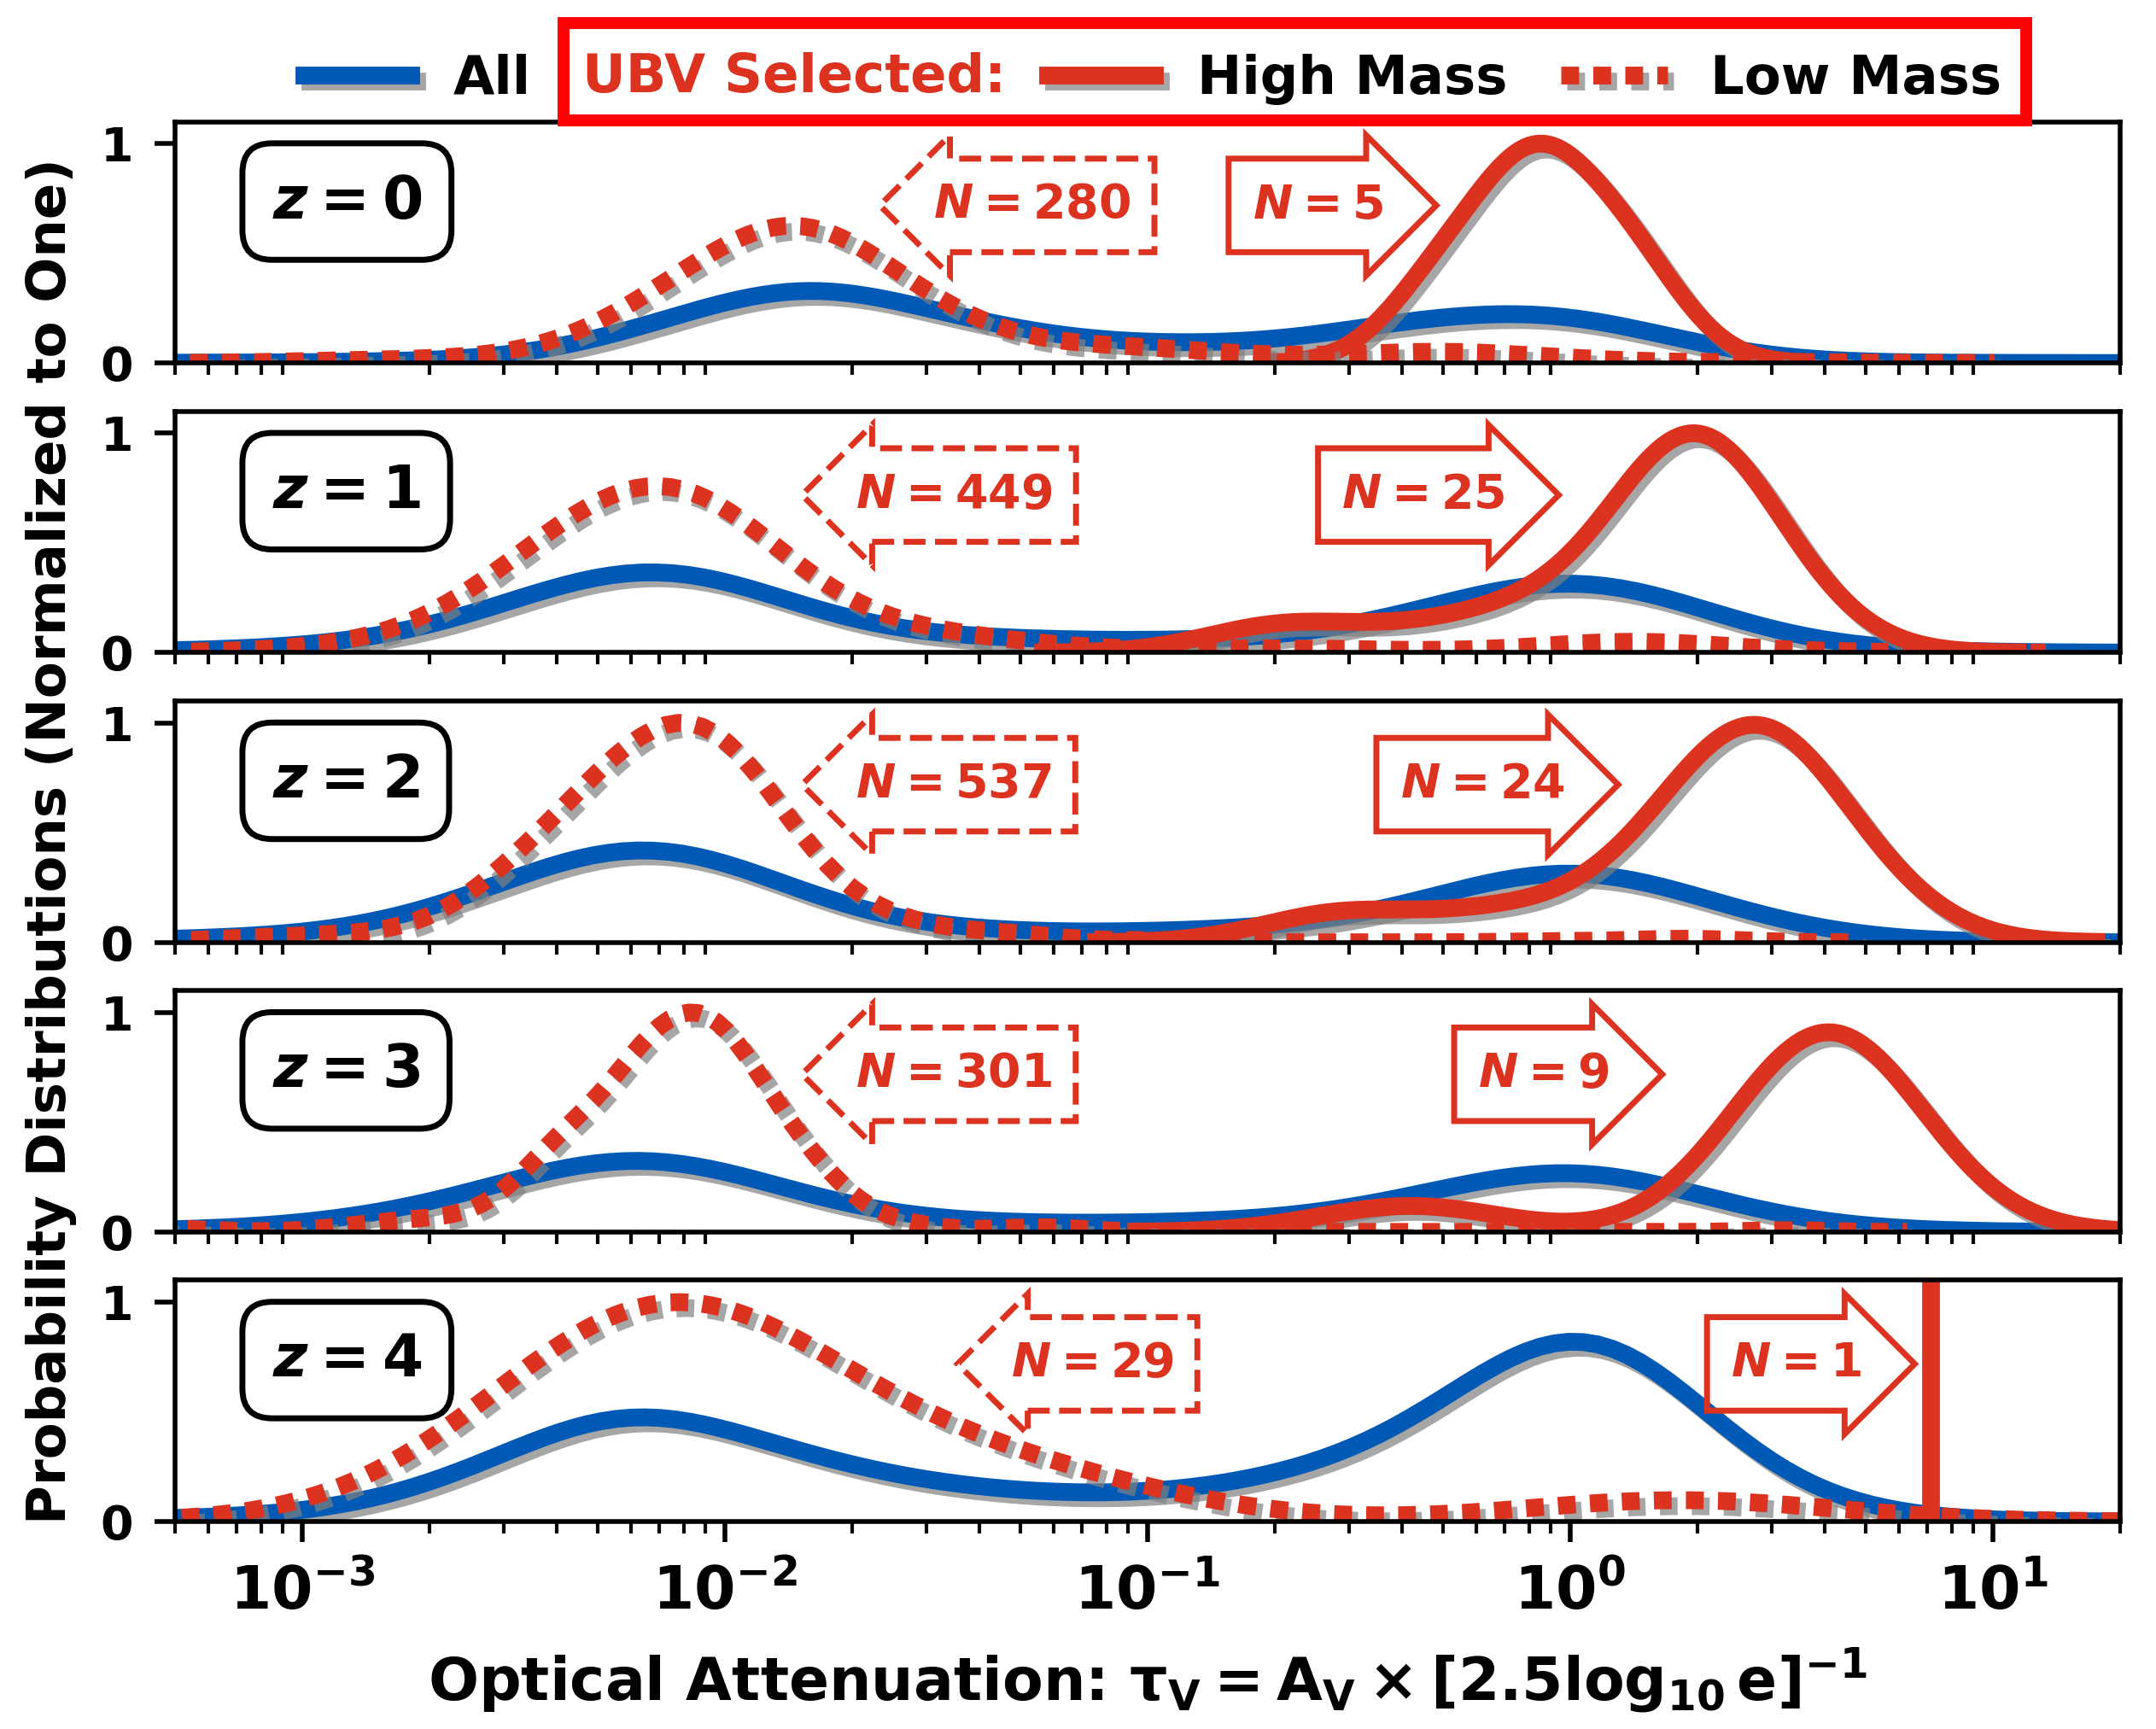
\includegraphics[width=\linewidth]{fig9_UBV_tauV.png}
    \caption{{\bf Molecular gas-rich massive (i.e. high mass; \eq \ref{eq:massLimit}) galaxies with PSB-like UBV colors are significantly more dust obscured than their low-mass (\eq \ref{eq:massLowLim}) counterparts.}  Here, we show distributions of the visual optical depth for galaxies, calculated from their attenuation curves.  While the blue line shows all galaxies in our sample, the red lines instead focus on those that satisfy our UBV classification (red dots in \fig \ref{fig:UBV}).  Such UBV-selected galaxies have further been divided into those that satisfy our high mass requirement from \S\ref{ssec:massLimit} (\eq \ref{eq:massLimit}; solid red line), and those that do not (\eq \ref{eq:massLowLim}; dotted red line), showing how our high-mass UBV-selected galaxies are dramatically more optically thick than their low-mass counterparts, with an increasing optical depth towards higher redshift.}
    \label{fig:observer}
\end{figure*}

While looking at \fig \ref{fig:IR_FUV}, it is instructive to ask why the UBV-selected galaxies on the right-most panel all have FUV-based SFR that underestimates the true SFR, and why only the high-mass galaxies (\eq \ref{eq:massLimit}) in the middle panel have an IR-based SFR that accurately traces the true SFR?  Both of these questions are answered in \fig \ref{fig:IR_FUV_GDR}, which shows the same ($z=0.5$) data as in \fig \ref{fig:IR_FUV}, now colored by the log ratio of the total gas-to-dust mass within each galaxy.  The latter question of why only the massive PSB-like galaxies have an IR-based SFR that traces their true SFR is answered by the left panel of \fig \ref{fig:IR_FUV_GDR} (same axes as in the middle panel of \fig \ref{fig:IR_FUV}).  Here, we see that the high-mass galaxies (\eq \ref{eq:massLimit}) that lie on the one-to-one line have very low gas-to-dust ratios, implying an abundance of dust, while those above the line have orders of magnitude higher values, thus are relatively dust-free \citep{Whitaker21b, Lorenzon25a, Spilker2025}; consequently, their IR-based SFR will underestimate their true SFRs.  In contrast, as the gas-to-dust mass ratio decreases towards the Milky Way value ($\sim$100) the points begin to fall closer to the one-to-one-line, implying that the IR luminosity only works as a SFR diagnostic near MW values of the gas-to-dust ratio.  These conclusions have been confirmed in the recent work by \cite{Spilker2025} and \cite{Lorenzon25b}.

The former question of why FUV-based SFR underestimates the SFR for all UBV-selected systems is investigated in the right panel of \fig \ref{fig:IR_FUV_GDR}.  Given that our UBV selection targets relatively dust-free galaxies, the FUV-derived SFR should be a robust tracer of star formation.  Although, if there is dust obscuration occurring in these systems, it follows that a hybrid or mixed SFR indicator might produce a SFR that is closer to the true value.  For example, \cite{Calzetti07} and \cite{Hao11} define the local ``gold standard" SFR by combining direct stellar light (FUV; 0.153$\mu m$) with a dust-emission-dominated luminosity ($24\mu m$).  Specifically, they define $\text{SFR(FUV+24}\mu \text{m)}/(\text{M}_\odot/\text{yr})=4.6\times 10^{-44}\left(\text{L}_{0.153\mu m}+6 \times \text{L}_{24\mu m}\right)/(\text{erg/s})$.  In the right panel of \fig \ref{fig:IR_FUV_GDR} we show how this mixed SFR measurement compares to the true SFR for our UBV-selected systems.  Here, we see that while this hybrid SFR measure does much better at tracing the true SFR than a purely FUV-based SFR (right-most panel of \fig \ref{fig:IR_FUV}), it still fails to recover the missing star formation in the lowest dust-mass systems (highest GDR).

While we have now shown that among those galaxies that satisfy the PSB-like UBV criteria at $z=0.5$, those that satisfy our high-mass cut (\eq \ref{eq:massLimit}) tend to be significantly more dust obscured than their low-mass counterparts (\eq \ref{eq:massLowLim}), we can continue to ask how this trend evolves with increasing redshift.  This is accomplished in \fig \ref{fig:observer}, in which for $z=0-4$ we plot the KDE distributions (re-normalized to one) of the visual optical depth\footnote{Note: We approximated $\tau_V$ by using the value of the total extinction at $\lambda=0.55\mu\text{m}=5500$\r{A}.  As a result, it follows that $\tau_V\equiv \tau_\lambda(0.55\mu\text{m})=\big(\frac{\ln{10}}{2.5}\big)\times A_\lambda(0.55\mu\text{m})$.} $(\tau_V\equiv A_V*[2.5\log_{10}\!{e}]^{-1})$.  Within each plot, we show the distribution of all galaxies in our simulation as a blue line, those that are UBV-selected and high mass (\eq \ref{eq:massLimit}) are shown as a solid red line, and those that are UBV-selected and low mass (\eq \ref{eq:massLowLim}) are shown as the dashed red line.  In \fig \ref{fig:observer}, we see that at all redshifts the high-mass galaxies have significantly higher $\tau_V$, thus are more dust obscured, than their low-mass counterparts.  Interestingly, between $z=0-3$, while the high-mass systems have an average $\tau_V$ that increases from $0.91$ to $3.71$, their low-mass counterparts actually have a decreasing average $\tau_V$ from $\sim 0.07\to 0.02$ over the same redshift range.  By $z=4$ we find that mostly all UBV-selected systems will be low mass (\eq \ref{eq:massLowLim}), due to the rarity of massive systems at these high redshifts (as discussed in \S\ref{ssec:massLimit}).

Collectively, the results of this section indicate that dust-obscured star formation may reasonably explain why observations are finding molecular gas in seemingly quenched galaxies.  Using observationally-based selection criteria, we analyzed a sample of PSB-like galaxies and have shown that while a SFR derived from the FUV will underestimate the true SFR for all such galaxies, the IR-based SFR instead will accurately trace the true SFR for gas-rich galaxies (yet still underestimate it for gas-poor galaxies).  We also found that such gas-rich galaxies will also have an abundance of dust, which lowers their gas-to-dust ratios towards MW-like values of $\sim 100$.  In summary, this section suggests that the seemingly quenched massive and molecular gas-rich (i.e. high mass; \eq \ref{eq:massLimit}) galaxies that exhibit PSB signatures instead contain dust-obscured star formation hidden in the galaxies center; surrounded by a quenched, dusty, and optically-thin outskirt that enshrouds the dust and exhibits PSB signatures.

\subsection{Putting it All Together}
\label{ssec:allTogether}
As shown in the last section (\S\ref{ssec:HC}), we have concluded that dust obscuration is the most likely mechanism for producing observations of molecular gas in seemingly quenched galaxies.  However, our investigation of the first hypothesis (\S\ref{ssec:HA}) also indicated that rejuvenation remains possible in high-mass galaxies that retain substantial molecular gas reservoirs, and have not yet fully quenched.  In this section we aim to connect these two hypothesis, and put them into the context of prior observational work  \citep{French_2018,Bezanson_2022,setton2025}.  In particular, we examine our results in the context of the observational inferences of massive H$_2$ reservoirs in PSB-like galaxies \citep{suess_2017}, and the rapid ($\sim150$ Myr) gas depletion time scales \citep{Bezanson_2022}.  

Specifically, \cite{setton2025} suggests that instead of requiring such rapid gas depletion timescales, an alternate explanation could be that their gas-rich and gas-poor `PSB-like' galaxies capture two distinct populations, or rather two separate evolutionary states.  Motivated by bright tidal features present in $\sim90\%$ of their gas-rich galaxies, they suggest that such galaxies could have just experienced a gas-rich merger which has imparted enough feedback to decrease their star formation efficiency and produce enough dust to make them temporarily appear quiescent.  In this picture, these gas-rich galaxies have not yet finished their life as star-forming galaxies and will rejuvenate again, whereas in contrast the gas-poor analogs of these would instead represent ``true" post-starburst galaxies that are entering into quiescence.

\begin{table}[H]
\vspace{-10pt}
\begin{deluxetable}{lccc}
\tablecaption{\textbf{Rejuvenation Fraction}\label{tab:rejuv}}
\tabletypesize{\small}
\setlength{\tabcolsep}{2pt}
\tablehead{
  \colhead{\textbf{Redshift}} &
  \colhead{\textbf{All}} &
  \colhead{\textbf{UBV Selected}} &
  % \colhead{\parbox[c]{1in}{\centering\textbf{All Galaxies}}} &
  % \colhead{\parbox[c]{1in}{\centering\textbf{UBV Selected}}} &
  \colhead{\parbox[c]{1in}{\centering\textbf{UBV Selected \& High Mass}}}
}
\startdata
$\bm{z = 0.5}$ & \textbf{14\%} {\footnotesize\textcolor{gray}{(140/972)}} & \textbf{11\%} {\footnotesize\textcolor{gray}{(23/204)}}  & \textbf{40\%}  {\small\textcolor{gray}{(2/5)}}   \\
$\bm{z = 1.0}$ & \textbf{24\%} {\footnotesize\textcolor{gray}{(285/1202)}}& \textbf{15\%} {\footnotesize\textcolor{gray}{(73/474)}} & \textbf{56\%}  {\footnotesize\textcolor{gray}{(14/25)}}  \\
$\bm{z = 2.0}$ & \textbf{48\%} {\footnotesize\textcolor{gray}{(881/1829)}} & \textbf{29\%} {\footnotesize\textcolor{gray}{(164/561)}}& \textbf{100\%} {\footnotesize\textcolor{gray}{(24/24)}}   \\
\enddata
\tablecomments{{\footnotesize Columns show rounded rejuvenation fractions for three
samples: all galaxies (`All'), UBV color-selected galaxies (`UBV Selected'), and
UBV-selected \& high-mass (\eq \ref{eq:massLimit}) galaxies (`UBV Selected \& High Mass').}}
\end{deluxetable}
\vspace{-50pt}
\end{table}

If the gas-rich galaxies from \cite{setton2025} do rejuvenate while their gas-poor counterparts quench, we should be able to see this behavior in our analogous sample, and in this section we will investigate this.  To accomplish this, we collect a sample of UBV-selected `PSB-like' galaxies at $z=0.5,1,2$ and followed them forward in time to see what fractions will rejuvenate, with results shown in Table \ref{tab:rejuv}.  In Table \ref{tab:rejuv}, we see that among UBV-selected galaxies, those that are also high mass (\eq \ref{eq:massLimit}) are significantly more likely to rejuvenate.  This effect is most pronounced at $z=2$, where we see that while only $\sim$30\% of UBV-selected galaxies will rejuvenate, when we restrict our sample to those UBV-selected galaxies that are also high mass (\eq \ref{eq:massLimit}), we find this fraction increases by $\sim 70\%$ to $100\%$.

While Table \ref{tab:rejuv} demonstrates that among UBV-selected galaxies, high-mass systems (\eq  \ref{eq:massLimit}) are significantly more likely to rejuvenate, \fig \ref{fig:rejuvComb} further shows that among high-mass galaxies, those with larger molecular gas fractions ($\mhh/M_*$) are considerably more likely to rejuvenate.  Taken together, this suggests that UBV-selected galaxies that are both massive and gas-rich at Cosmic Noon are the most likely candidates for rejuvenation.  This paints a picture in which on average, the massive gas-rich UBV-selected (`PSB-like') galaxies could come back to life, produce a starburst, then transition to a gas-poor (`true') PSB system, which will ultimately quench fully.  To investigate this hypothesis further, we apply the photometric selection method from \S\ref{ssec:HC} to the example of a rejuvenating galaxy we initially investigated in \fig \ref{fig:rejuvCase}, and identify the snapshots at which it would be classified as `PSB-like' by the UBV selection (\eq \ref{eq:UBVSelect}), with results shown in \fig \ref{fig:rejuvCaseUBV}.

\begin{figure}
    \centering
    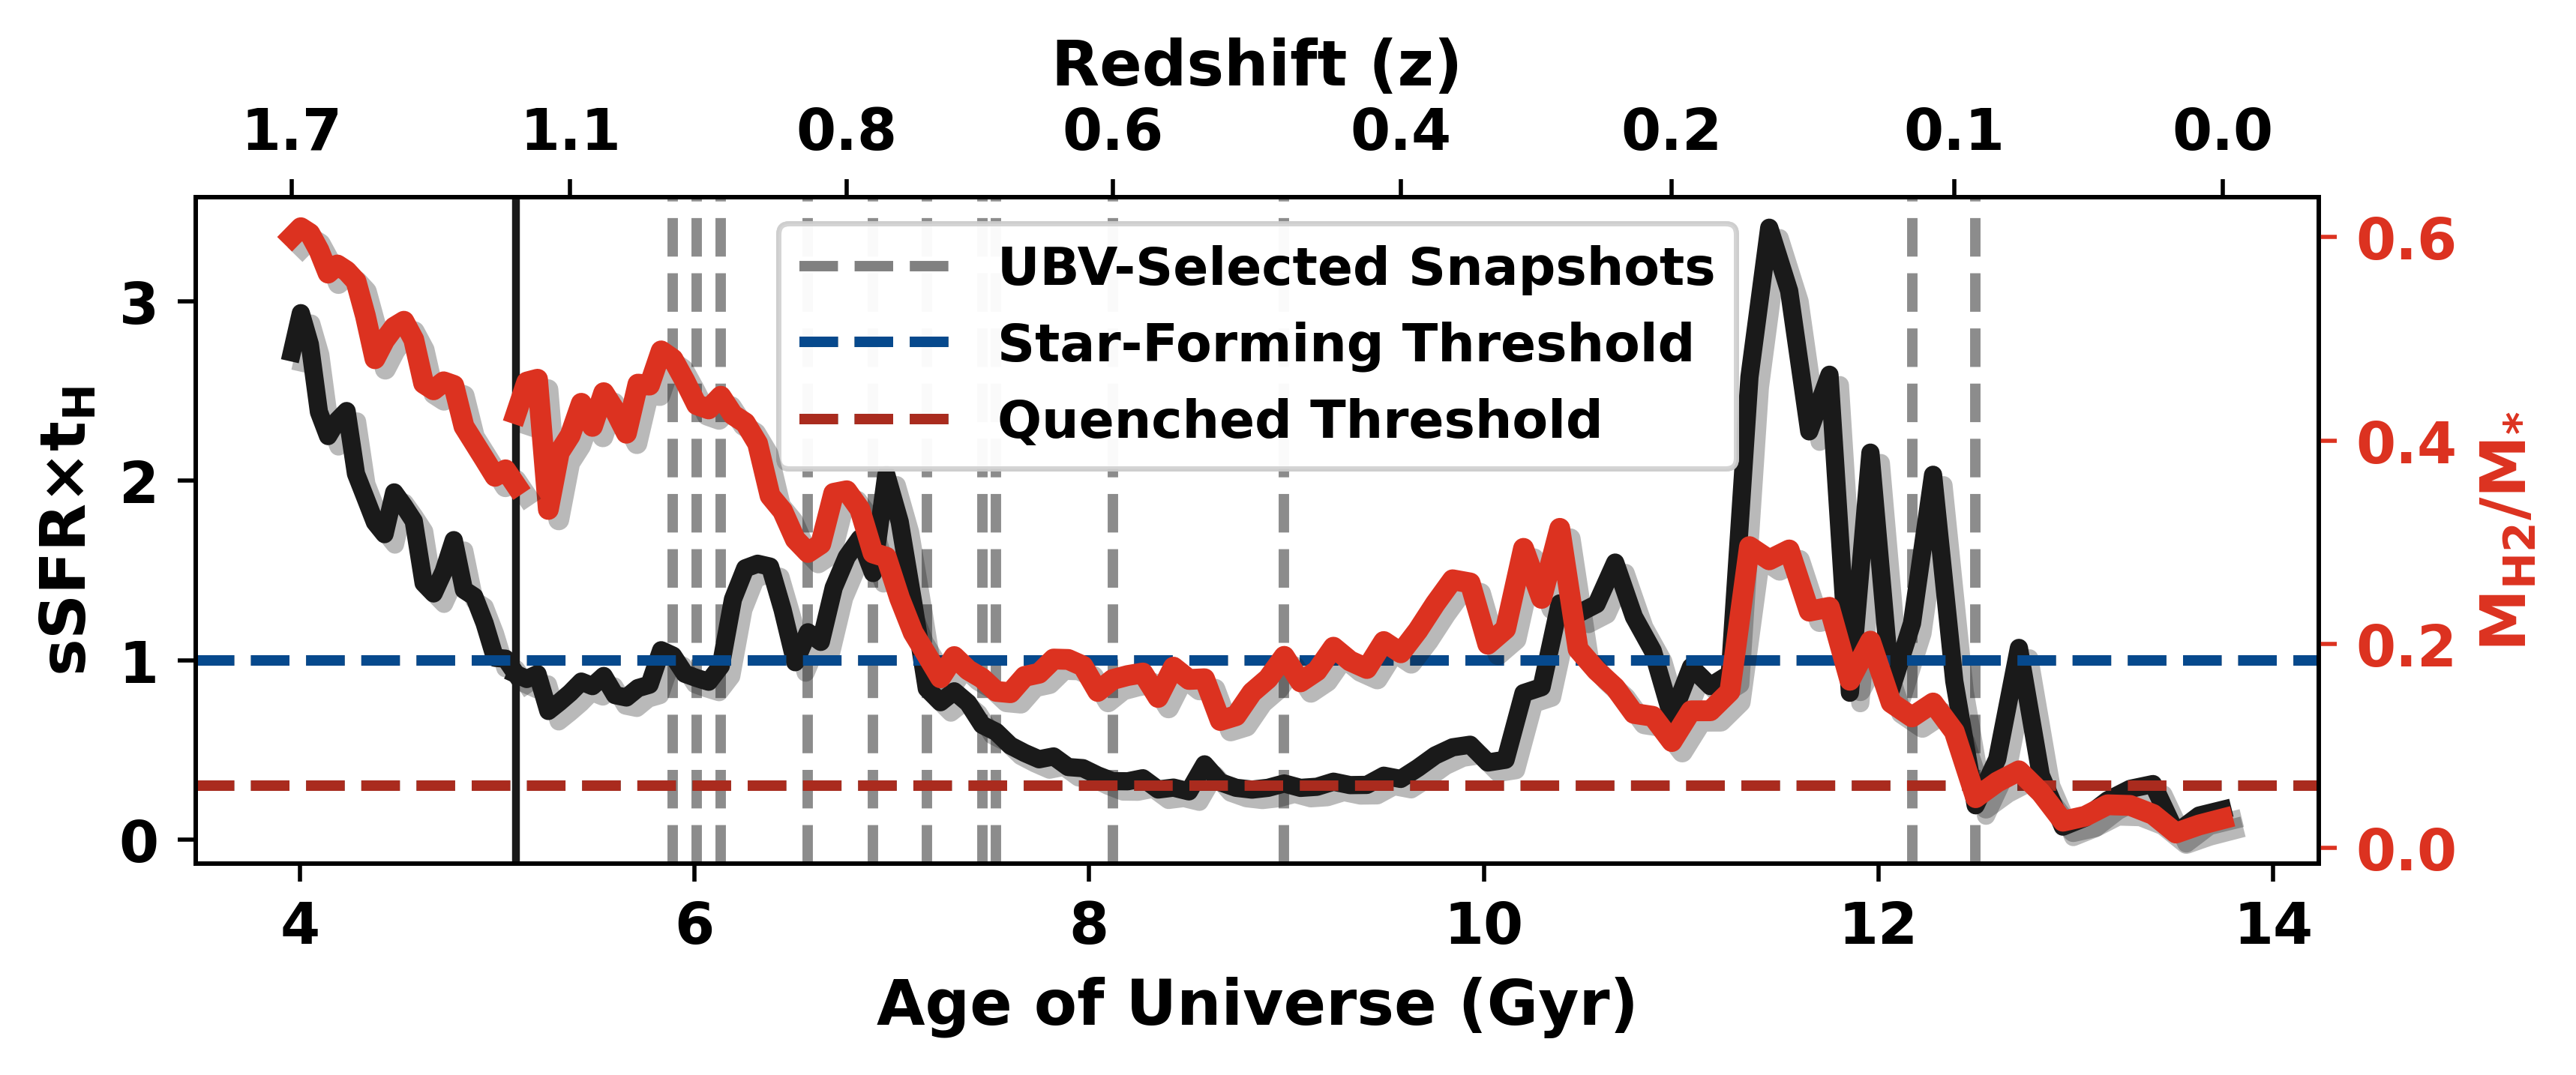
\includegraphics[width=\linewidth]{figNewSect_rejuvCaseUBV(2).png}
    \caption{{\bf The example rejuvenating galaxy, originally shown in \fig \ref{fig:rejuvCase}, will be UBV-selected many times (dashed vertical lines) before finally quenching.}  Initially selected at at $z\sim1.2$ (solid black line; $\tH\sim5.1$ Gyr), the galaxies $\ssfr\times \tH$ is shown as a solid black line (values on left $y$-axis).  The solid red line shows the associated molecular gas-to-stellar mass ratio, with values on the right $y$-axis. Here we broadly see that when this high-mass galaxy is UBV selected and gas-rich $(\mhh/M_*>0.1)$, it will rejuvenate $(\tH<10\text{  Gyr})$, but when its UBV selected and gas-poor $(\tH>11\text{ Gyr})$, it will quench fully.}
    \label{fig:rejuvCaseUBV}
\end{figure}

Within \fig \ref{fig:rejuvCaseUBV}, after initially selecting our model galaxy at $z\sim1.2$ (solid black line; $\tH\sim5.1$ Gyr), we tracked it forward in time, and have marked every snapshot in which it would be UBV selected for all viewing angles via a vertical dashed line.  As in \fig \ref{fig:rejuvCase}, the black line (left $y$-axis) shows the model galaxy's $\ssfr\times \tH$, and the blue and red horizontal dashed lines show the star-forming and quenching thresholds respectively (\eq\ref{eq:ssfrt1}/\ref{eq:ssfrt3}).  In addition, we also show the molecular gas-to-stellar mass ratio as a red line, with associated values shown on the right $y$-axis.  From \fig \ref{fig:rejuvCaseUBV}, we see on first glance that UBV classification does not directly imply the galaxy will quench.  Indeed, this galaxy would have been UBV selected ten times for $\tH<10$ Gyr, prior to its major rejuvenation event.  Only after this major merger driven rejuvenation event do we again see it fall under our UBV classification, around $\tH\sim 12$ Gyr, at which point its SFR and molecular gas-to-stellar mass ratios finally will decrease towards zero as the galaxy finally quenches.


Taken together, the cumulative evidence presented thus far demonstrates that a galaxy which has already undergone an initial burst of star formation can have dust from this prior event obscure ongoing star formation, causing the galaxy to exhibit photometric colors characteristic of `PSB-like' galaxy.  Even when such a galaxy has a decreased star-forming efficiency due to feedback, if it still has a significant molecular gas-to-stellar mass ratio ($\mhh/M_*>0.1$), then this galaxy could still rejuvenate.  Only when it has depleted most of its molecular gas will it ultimately transition to being fully quenched.  In other words, among our sample of UBV-selected and high-mass galaxies (\eq \ref{eq:massLimit}/\ref{eq:UBVSelect}), those that are massive and molecular gas-rich are significantly more likely to rejuvenate then their gas-poor or low-mass counterparts, which are far more likely to fully quench.

While this mechanism could reasonably explain why observations are finding molecular gas in seemingly quenched galaxies, it does not explain the observed rapid $(\sim150 \text{ Myr})$ disappearance of $\mhh$.  For example, while dust obscuration can hide residual star formation, given the $\sim$ Gyr timescales associated with gas depletion in these systems, this ongoing star formation cannot deplete the remaining gas fast enough.  While rejuvenation has been suggested as an alternative mechanism to this rapid gas depletion \citep{setton2025}, our example of a rejuvenating galaxy shown in \fig\ref{fig:rejuvCaseUBV} is not able to accomplish this H$_2$ depletion on the required timescales.  

One caveat is that this result may reflect the absence of bursty star formation in our simulation, which could play a key role in driving rapid molecular gas depletion.  In our \simba model, this restriction arises from the artificial pressurization of the ISM imposed by our effective equation of state \citep{simba}.  Implemented as a subgrid model in order to resolve the Jeans mass within our large-box volume \citep{mufasa}, this self-regularizing ISM acts to reduce star formation and prevent bursts.  We leave a more in depth statistical investigation into this mechanism for future studies.

\newcommand{\firebox}[0]{{\sc FIREbox} }
\newcommand{\fire}[0]{{\sc fire}}
%\newcommand{\cenci}[0]{Cenci et al., 2025 (in prep) }
\newcommand{\cenci}[0]{\cite{cenci25} }
%========================== New Discussion ==========================
\section{Discussion: Comparison to Other Theoretical Models}
\label{sec:discussion}
Large-volume hydrodynamic simulations such as \simba have had great success in the past in reproducing many of the statistical trends seen in observations.  Cosmological simulations such as these thus provide a potentially powerful avenue towards learning how massive galaxies can preserve their molecular gas reservoirs after star formation shuts off.  Throughout this paper we used the \simba simulation to investigate how molecular gas reservoirs could persevere in recently quenched massive galaxies.  

To place our results in the context of previous work, this section reviews other theoretical studies of analogous systems, namely post-starburst galaxies (PSBs), as introduced in the introduction (\S\ref{sec:intro}).  There are two major theoretical studies investigating the origin of molecular gas in PSBs.  First, \cite{psbEagle} used the \eagle simulations to investigate the molecular gas properties of PSBs, and secondly, \citet{cenci25} studied PSBs with the \firebox simulation \citep{firebox}, which is part of the \textit{Feedback in Realistic Environments} (\fire) project \citep{fire, fire2}.

In terms of galaxy selection criteria, \cite{psbEagle} identified their sample of PSB galaxies in \eagle by focusing on massive ($M_*>10^{9.5}M_\odot$) galaxies, initially star forming ($\ssfr>5\times 10^{-11}yr^{-1}$), that experienced at least a factor of 5 drop in sSFR within 600 Myr.  In contrast, \cenci instead first used the same UBV-selection criteria applied in \S\ref{ssec:HC} to the central galaxies in \firebox with $M_*\ge 5\times 10^9 M_\odot$ to define their sample of PSB galaxies.  A `true PSB' was then defined to be any such system with $\text{sSFR}<3\times 10^{-11} \textrm{yr}^{-1}$, that also experienced a least a factor of four drop in their SFR since their most recent starburst, while an `impostor PSB' would be any photometrically selected PSB that does not satisfy these additional criteria (i.e. star-forming UBV-selected systems).  This approach effectively combines aspects of our sSFR-based galaxy selection criteria described in \S\ref{ssec:select} with the photometric selection method we used in \S\ref{ssec:HC}.

Using these selection criteria, \cenci found that among their star-forming galaxies, around 8.7\% at $z=0.7,1.0$ would be classified as `imposter PSBs', thus instead represent star-forming systems misclassified as PSBs due to their photometry, and will contain substantial molecular gas reservoirs with depletion times of 600 Myr -- 1.2 Gyr.  In contrast, those identified as `true PSBs' (quenched and UBV selected) will be gas-poor, and will exhibit the longest depletion times.  Similarly, \cite{psbEagle} found that the average PSB in \eagle\! loses $\sim 90\%$ of its star-forming ISM within $\sim$600 Myr following the starburst.  Putting this into the context of our example rejuvenating galaxy shown in \fig \ref{fig:rejuvCase}/\ref{fig:rejuvCaseUBV}, which undergoes a merger-driven starburst at $\tH \sim 11$ Gyr (see \app \ref{app:merge}), we see 600 Myr later the system has lost $\sim50\%$ of its $\hh$ mass, and only 1.2 Gyr after this major starburst has 90\% of its $\hh$ mass been depleted.


\cenci showed that typical PSBs, despite representing only 9.2\% of galaxies at $z=1$, tend to have molecular gas contents similar to star-forming galaxies of similar mass.  Among these systems, they find that only $\sim$10\% would be classified as `true PSBs'.  They find such systems to be significantly gas-poor, with typical gas resevoirs likely below the detection limits of current observational facilities, making these systems virtually undetectable.  Since a majority of PSBs in \eagle retain significant molecular gas reservoirs \citep{psbEagle}, it would follow that such systems instead constitute a sample of `imposter PSBs', who have recently experienced a wave of feedback which has temporarily reduced their star forming efficiency.  This is in line with their findings that such PSBs contain highly disturbed gas, with only a small fraction of kinetic energy in ordered rotation \citep{psbEagle}.


In the context of this study, it follows that in our analogous sample of UBV-selected `PSB-like' galaxies defined in \S\ref{ssec:HC} (shown in \fig \ref{fig:IR_FUV}), those high-mass galaxies (red stars) would be defined as `impostor PSBs'.  As discussed in \S\ref{ssec:HC}, such systems have cores containing obscured star formation, surrounded by dusty outskirts that make their photometry resemble typical PSBs. Furthermore, as discussed in \S\ref{ssec:allTogether}, among such high-mass (\eq\ref{eq:massLimit}) and UBV-selected (\eq\ref{eq:UBVSelect}) systems, those that are also molecular gas rich are significantly more likely to rejuvenate when tracked forward in time.  It follows that the low-mass (\eq\ref{eq:massLowLim}) UBV-selected galaxies (red dots in \fig \ref{fig:IR_FUV}) then represent our sample of `true PSBs', and will instead fully quench when tracked forward in time.  

The results from this section and the previous one highlight that, in addition to the traditional photometric methods used to identify PSBs, to avoid including systems with dust-obscured ongoing star formation (`imposters'), one must incorporate additional selection criteria that focuses on their current level of star formation (in addition to their photometry).
%========================== Conclusion ==========================
\section{Conclusion}
\label{sec:conclusion}
The aim of this paper was to holistically investigate various hypotheses that could give rise to observations of massive $(M_*>10^{10}M_\odot)$ and quenched galaxies harboring significant molecular gas reservoirs $(\mhh>10^{9}M_\odot)$ such as those from \cite{rowlands, french_2015, suess_2017, Bezanson_2022, setton2025}.  The approach we took utilized the \simba hydrodynamic galaxy-formation simulations, whose novel multi-scale prescriptions have made it one of the best modern simulations for exploring galaxy evolution and baryon cycling within a cosmological context \citep{simba}.  Cosmological simulations such as this provide a powerful laboratory capable of studying the intricate interplay between a galaxy and its ISM, allowing in-depth investigations into their coevolution and the driving mechanisms connecting them.  

While many studies have individually considered hypotheses that could give rise to observations of quenched galaxies that still harbor reservoirs of molecular gas, this study is meant to holistically investigate each within a singular cosmological simulation, providing a self-consistent analysis of the relative role of each theory across space and time.  We investigated three hypotheses in total; the first of which asking about temporal effects intrinsic to the galaxy (\S\ref{ssec:HA}), while the last two deal with observational effects.  Specifically, our second hypothesis asks if the galaxy truly contains molecular hydrogen (\S\ref{ssec:HD}), while the third asks if the galaxy is truly quenched (\S\ref{ssec:HC}).

Our main results are as follows.
\begin{itemize}[nosep]
    \vspace*{.05in}
    \item Hypothesis \#1 (\S\ref{ssec:HA}):  quenched galaxies harboring molecular gas could reignite their star formation after a period of quiescence.  We showed that while rejuvenation is an important merger-driven effect at high redshift (\fig \ref{fig:rejuvCase}), primarily occurring for those molecular gas-rich galaxies that are not yet fully quenched (\fig \ref{fig:rejuvComb}), it reduces in relative likelihood at low redshift (\fig \ref{fig:rejuv}).
    \vspace*{.1in}
    \item Hypothesis \#2 (\S\ref{ssec:HD}):  the common assumption that the $\aco$ value derived in the Milky Way ($\acomw$) applies to all galaxies is what is leading to an overestimation of the molecular gas mass in quenched galaxies. In \fig \ref{fig:alphaCO}, we showed that $\aco<\acomw$ for all galaxies, regardless of their mass or star formation classification.  Thus, the results of this hypothesis does not help answer why observers find molecular gas in quenched galaxies, but rather suggests that the scaling relations for all galaxies must be shifted to solve this discrepancy.
    \vspace*{.1in}
    \item Hypothesis \#3 (\S\ref{ssec:HC}):  dust obscuration could hide star formation, causing these galaxies to be improperly labeled as `not star forming'.  Focusing on those galaxies that satisfy PSB-like quenching signatures (red dots in \fig \ref{fig:UBV}), we show in \fig \ref{fig:IR_FUV} that those systems that are also massive and molecular gas-rich (red stars) will have an IR-based SFR that accurately traces their true SFR, yet an FUV-based SFR that underestimates it.  This indicates that the UBV-selected molecular gas-rich (i.e.\,high mass; \eq\ref{eq:massLimit}) systems could have star formation occurring deep within the galaxy, enshrouded by a quenched and dusty outskirt, with increasing levels of obscuration as redshifts increase from $z=0\to 4$ (\fig\ref{fig:observer}). This associated abundance of dust is confirmed in \fig \ref{fig:IR_FUV_GDR}, where we show that the gas-to-dust ratios of such systems are as low as those of the Milky Way ($\sim 100$) at $z=0.5$.
    \vspace*{.1in}
    \item Putting It All Together (\S\ref{ssec:allTogether}): among those UBV-selected galaxies from \S\ref{ssec:HC}, those that are also high-mass (\eq\ref{eq:massLimit}) are significantly more likely to rejuvenate than their low-mass counterparts (Table \ref{tab:rejuv}).  These results, combined with the insight gained from using our UBV classification (\eq\ref{eq:UBVSelect}) to identify where our example of rejuvenating galaxy appears `PSB-like' (\fig \ref{fig:rejuvCaseUBV}), suggests that the gas-rich subset of our high-mass UBV-selected galaxies constitutes a population of `imposter' PSBs (\S\ref{sec:discussion}) that are likely to undergo rejuvenation.  By contrast, their low-mass or gas-poor counterparts are more likely to represent the `true' PSB population, and to proceed toward full quenching when evolved forward in time.
\end{itemize}
\vspace*{.05in}

By investigating all three hypotheses, we have come to the conclusion that the most likely mechanism for producing observations of recently quenched high-mass galaxies with persistent molecular gas reservoirs is dust obscuration (Hypothesis 3: \S\ref{ssec:HC}), suggesting that a galaxy with enough gas and dust can be perceived by an observer as quenched despite still harboring obscured star formation.  In our discussion we put these results into the context of recent theoretical studies to show that such high-mass UBV-selected systems would actually be classified as `imposter' PSBs due to their abundant and persistent molecular gas reservoirs.  

Beyond this, in \S\ref{ssec:allTogether}, we showed that high-mass UBV-selected galaxies are significantly more likely to rejuvenate than their low-mass counterparts, especially at $z=2$, implying a general bimodal model of PSB-like systems.  Here, those photometrically selected systems that are high-mass or gas-rich are `imposter' PSBs that instead could rejuvenate, experience an extreme starburst event that depletes its molecular gas resevoirs; only after which it would again become UBV selected and enter into the `true' PSB population, defined by their low mass and gas-poor ISM, which will fully quench.  While existing observations seem to support this picture \cite{setton2025}, more results from ALMA are needed to investigate this physical scenario.
%========================== Acknowledgments ==========================
\begin{acknowledgments}
\textbf{Acknowledgments}

\noindent
D.N., R.B. and J.G. are grateful for funding from the NSF via grant AST-1908137.  E.S. was additionally funded via grant NASA ADSPS23-0007.  The authors acknowledge UFIT Research Computing for providing computational resources on HiPerGator and support that have contributed to the research results reported in this publication (\url{http://it.ufl.edu/rc}).
\end{acknowledgments}


%========================== Bibliography ==========================
%\bibliographystyle{abbrv}
\bibliography{bib}

\appendix
\section{A: Merger-Driven Rejuvenation}
\label{app:merge}
In \S\ref{ssec:HA}, while investigating whether the observed molecular gas in quenched galaxies could be due to them experiencing a temporary period of dormancy, followed by a rejuvenation, we stated that the rejuvenation event shown in \fig \ref{fig:rejuvCase} was driven by a major merging event.  In this section, we provide proof of this by visually examining the galaxy at various points in time.  To accomplish this, we pick nine points of interest during our galaxies evolution and show a projection plot of the gas density for each (shown in \fig \ref{fig:rejuvABC}-\ref{fig:rejuvGHI}), labeled with a letter (A-I) that corresponds to the time/redshift indicated by the same letter in the middle of \fig \ref{fig:rejuvLetters}.

\begin{figure}[h]
    \centering
    
\includegraphics[width=\linewidth]{fig11_rejuvLabeled.png}
    \caption{{\bf Example of a rejuvenating galaxy from \fig \ref{fig:rejuv}, with added letters (A-I) corresponding to the images in Figs. \ref{fig:rejuvABC}-\ref{fig:rejuvGHI}.}  This galaxy was selected at $z\approx 1.2$ ($\tH\sim 5.1$\,Gyr), based on it satisfying both our conditions for being low star-forming (\eq \ref{eq:ssfrt4}) and high mass (\eq \ref{eq:massLimit}), with the background color set to the star-forming classification of the galaxy based on \eq \ref{eq:ssfrt1}-\ref{eq:ssfrt3}.  While the top panel shows the evolution of $\ssfr\times \tH$, the bottom panel shows the corresponding evolution of $\hh$ mass (left/black) and stellar mass (right/red), both of which show a gradual evolution at high redshift, followed by a dramatic increase at around $z\approx 0.3$ driven by a major merging event.  The drop-off after this and subsequent rise show that the merging galaxy initially passes through our main galaxy, but, now bound within its potential well, later falls back and ultimately merges.}
    \label{fig:rejuvLetters}
\end{figure}

As a reminder to the reader, in \fig \ref{fig:rejuvLetters} (as in \fig \ref{fig:rejuvCase}; \S\ref{ssec:HA}), the top panel shows the quantity we used to classify the galaxy's current state of star formation (i.e. $\ssfr\times \tH$; see \S\ref{ssec:select}), thus has two horizontal lines located at (a) the star-forming cut (\eq \ref{eq:ssfrt1}: $\ssfr\times \tH=1$) and (b) the quenching threshold (\eq \ref{eq:ssfrt3}: $\ssfr\times \tH=0.3$).  The background color in both panels reflects this classification, with blue regions showing where the system would be considered `star-forming', yellow for `transitioning', and red for `quenched'.  To investigate the external processes that influence this galaxies evolution, we picked nine illustrative moments across time and produced a projection plot of the gas density in our galaxy for each (\fig \ref{fig:rejuvABC}-\ref{fig:rejuvGHI}) via \yt \citep{yt}, an astrophysical analysis and visualization toolkit.

After selecting our galaxy to be both low star-forming and high mass at a redshift of $z=1.2$ ($\tH\sim 5.1$ Gyr), we begin our exploration of this galaxies evolution at a redshift of $z=1.10$ (labeled `A'; $\tH\sim 5.54$ Gyr), in which the galaxy has finished decreasing its SFR, after being an originally gas-rich star-forming galaxy, and is now in the `transitioning' phase of star formation (\eq\ref{eq:ssfrt2}).  At this point we also see a small interloper galaxy is trapped in our galaxies potential well (bottom left of the image labeled `A' in \fig \ref{fig:rejuvABC}).  As we can see in both images `A' and `B' (\fig \ref{fig:rejuvABC}), this close encounter produces tidal tails in our galaxy and, as shown in \fig \ref{fig:rejuvLetters}, also causes a small burst in star-formation starting around 6 Gyr, temporarily shifting our galaxy into the `star-forming' region (image `B'; $z\sim0.9$).  Eventually, this interloper merges with our target galaxy, disrupting its spiral structure (as shown in image `C'; \fig \ref{fig:rejuvABC}), heating the gas and quenching star formation at around 7 Gyr ($z\sim 0.8$), at which point our galaxy is demoted back to `transitioning' (\eq\ref{eq:ssfrt2}).

\begin{figure}[H]
    \centering
    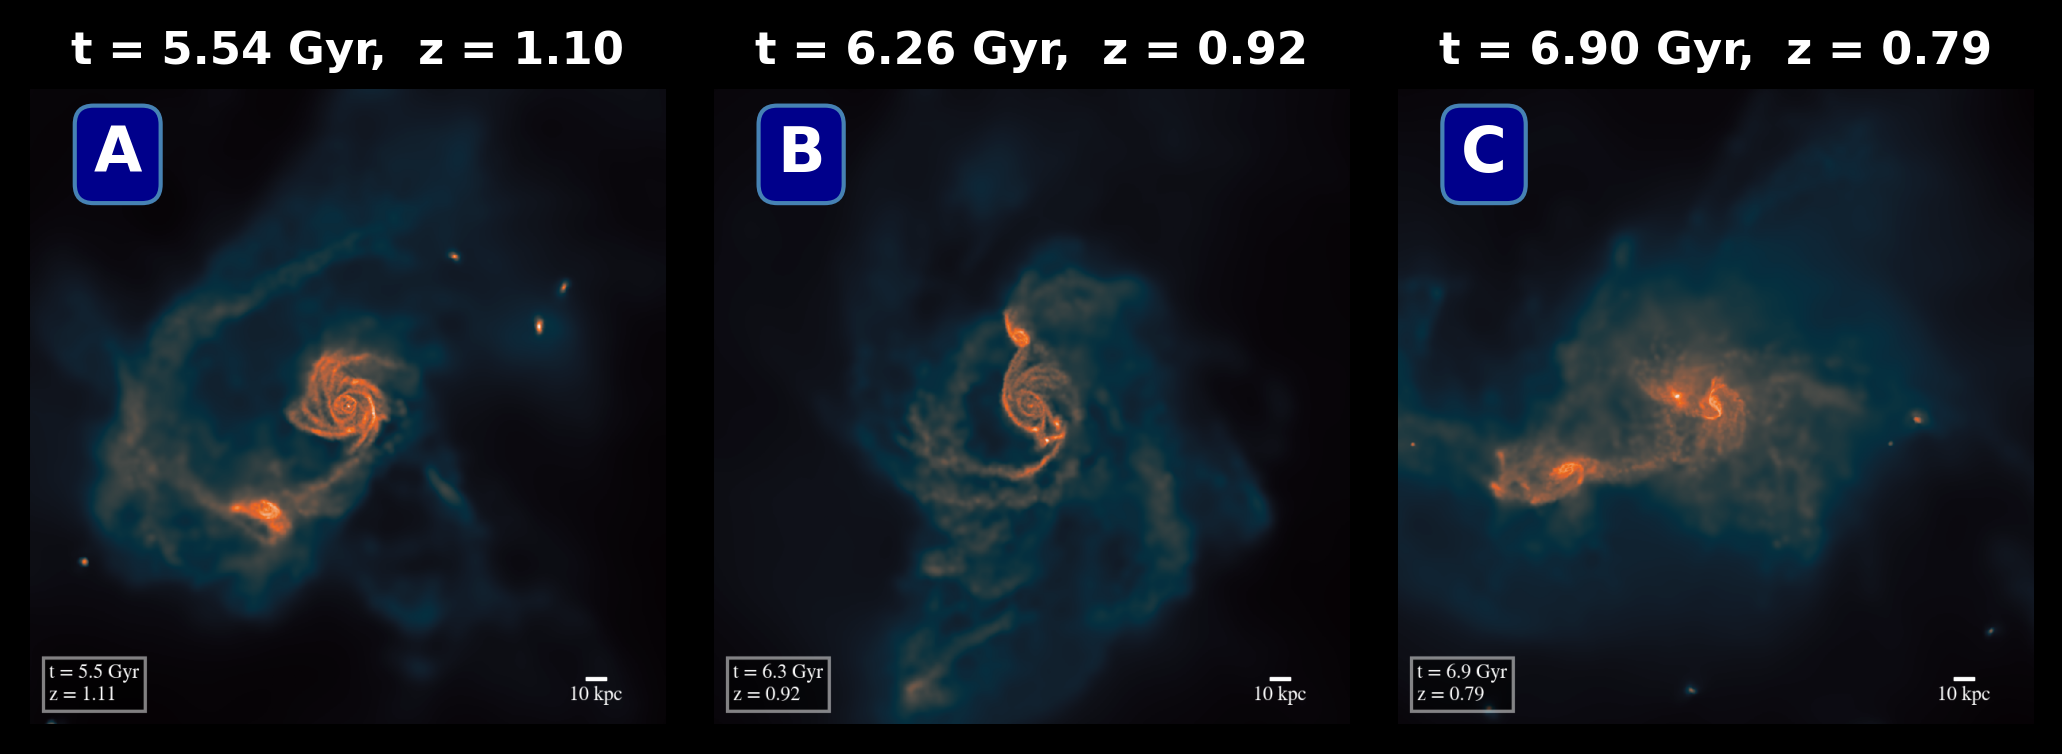
\includegraphics[width=.8\linewidth]{imgsABC.png}
    \caption{\textbf{A}: companion system enters the orbit of our quenching galaxy; \textbf{B}: interloping dwarf system triggers tidal tails and small burst in star formation; \textbf{C}: interloping system falls into our target galaxy, disrupting star formation and destroying its spiral structure}
    \label{fig:rejuvABC}
\end{figure}  

After this disruption, as the circumgalactic gas cools it gradually begins to fall back into the galaxy.  Eventually, at around 8 Gyr ($z\sim 0.6$), our galaxy begins to regain its spiral structure (image `D': \fig \ref{fig:rejuvDEF}). Approximately $1$ Gyr later ($\tH=9$ Gyr, $z\sim0.5$) is when our galaxy achieves its most ordered rotation and begins to resemble a grand design morphology (image `E'; \fig \ref{fig:rejuvDEF}).  Despite being defined as `quenched' (\eq\ref{eq:ssfrt3}) at this point using our sSFR-based classification scheme from \S\ref{ssec:select} (as shown at the point labeled `E' in \fig \ref{fig:rejuvLetters}), our galaxy still has enough molecular gas to be detectable via CO according to \eq \ref{eq:massLimit} (\S\ref{ssec:massLimit}).  Furthermore, after this point (labeled `E' in \fig \ref{fig:rejuvLetters}) this molecular gas has settled back into the galaxy enough to cause the SFR to gradually begin to increase.

\begin{figure}[H]
    \centering
    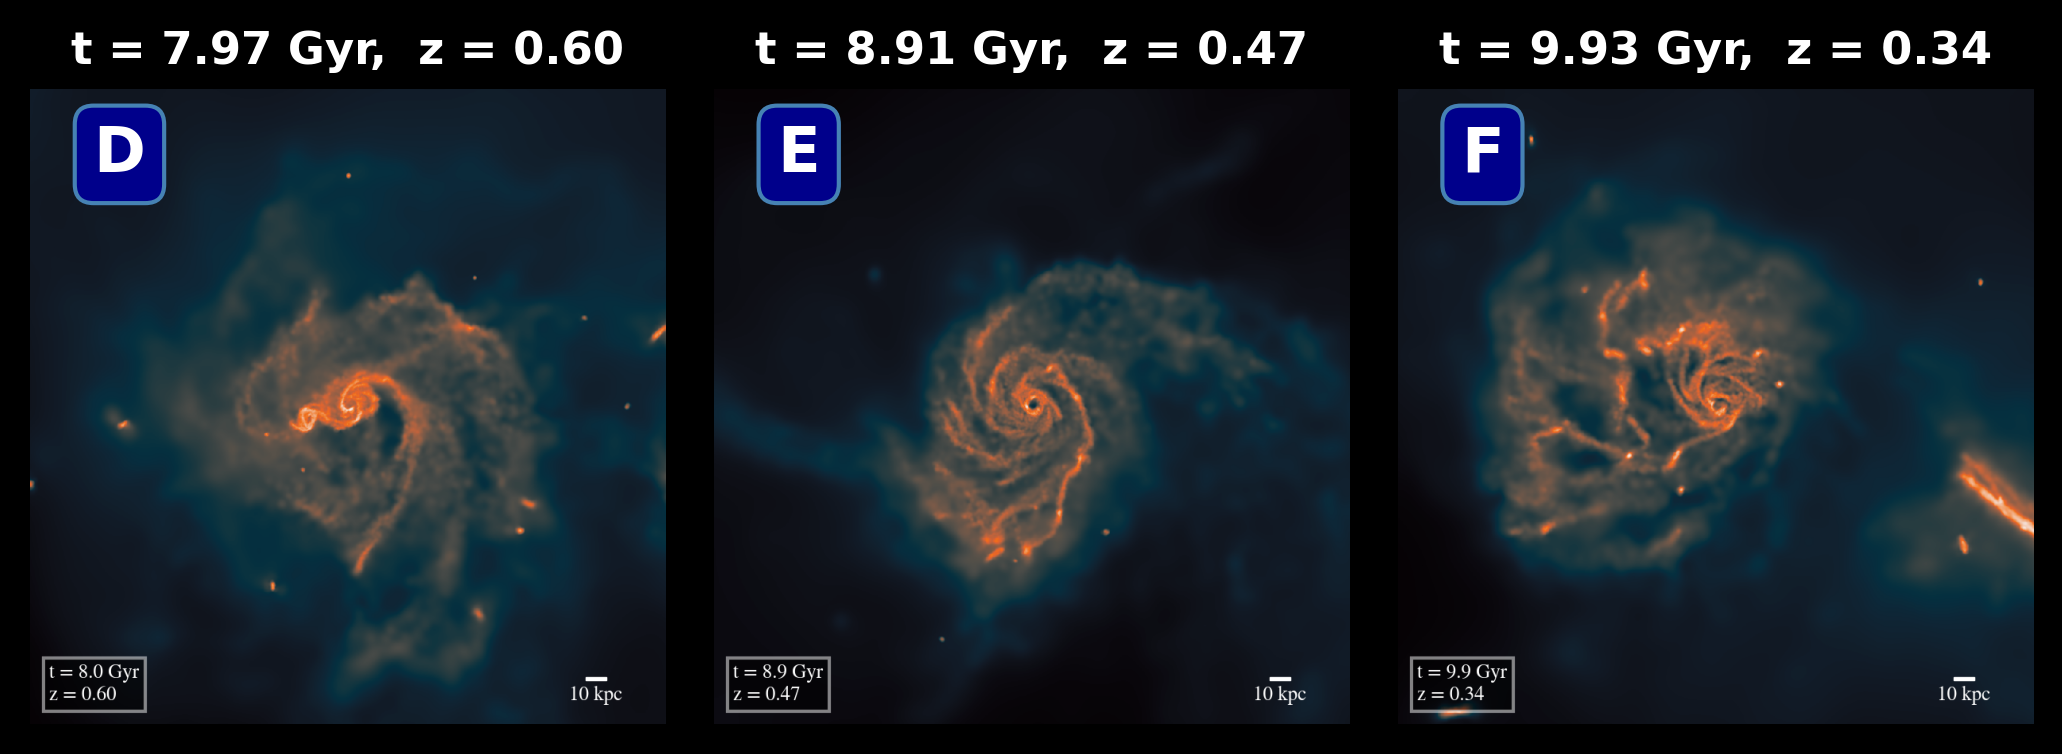
\includegraphics[width=.8\linewidth]{imgsDEF.png}
    \caption{\textbf{D}: gas begins to fall back into gravity well as spiral structure is regained; \textbf{E}: settling galaxy regains complete spiral structure; \textbf{F}: merging galaxy appears in the projection plot in the bottom right}
    \label{fig:rejuvDEF}
\end{figure}  

Moving forward in time by another Gyr ($\tH\sim 9.9$ Gyr, $z\sim 0.35$) allows us to see the point when another massive galaxy appears to be headed directly towards our target galaxy (as shown in the bottom-right of image `F' in \fig \ref{fig:rejuvDEF}).  Around 250 Myr later this galaxy eventually collides with our target system, and we can see the moment before impact in image `G' in \fig \ref{fig:rejuvGHI}.  At this point in \fig \ref{fig:rejuvLetters} (`G'; $\tH\sim 10.2$ Gyr, $z\sim 0.32$) we see a corresponding increase in SFR triggered by the tidal forces of the incoming galaxy.  Moving rightwards of this point in \fig \ref{fig:rejuvLetters} we see the galactic collision at $\tH\sim 10.4$ Gyr ($z\sim 0.3$) triggers a dramatic increase in both $\mhh$ and $M_*$, and a small burst in $\sfr$.

\begin{figure}[H]
    \centering
    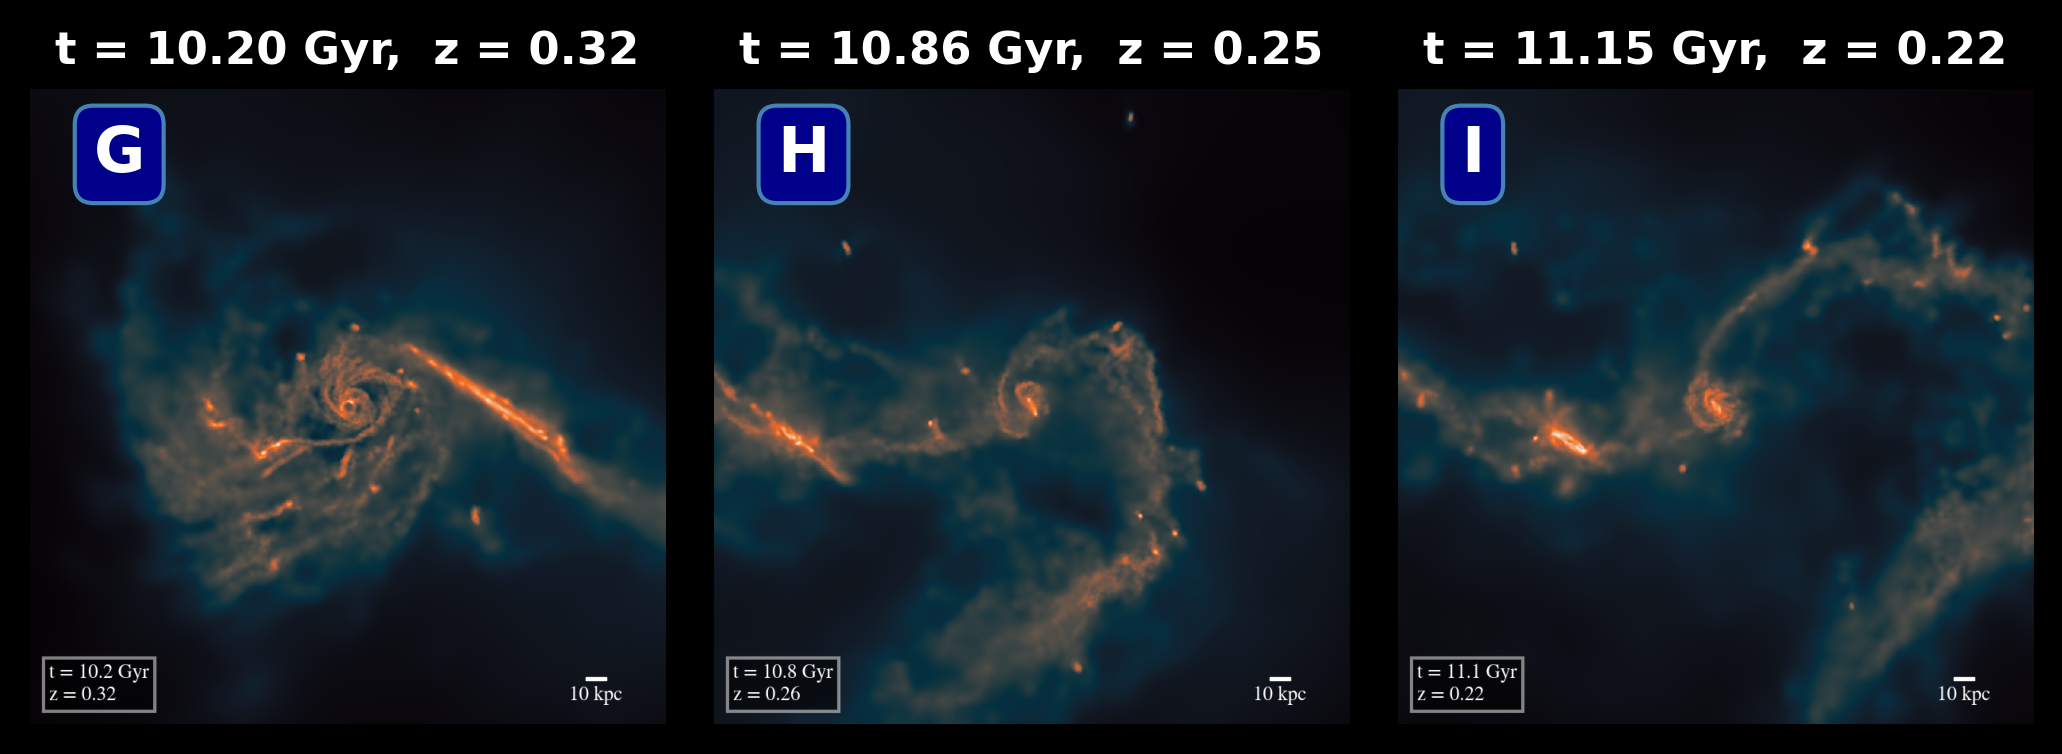
\includegraphics[width=.8\linewidth]{imgsGHI.png}
    \caption{\textbf{G:} merging galaxy makes first contact with our target galaxy; \textbf{H}: merging galaxy passes through and past our target galaxy; \textbf{I}: merging galaxy eventually falls back into our target galaxy}
    \label{fig:rejuvGHI}
\end{figure}  


After initially colliding with the main galaxy at $10.4$ Gyr, we see that the secondary system passes through and past our target galaxy (as shown in image `H' in \fig \ref{fig:rejuvGHI}).  At the corresponding point labeled `H' in \fig \ref{fig:rejuvLetters} ($\tH=10.86$ Gyr, $z= 0.25$), we see this causes the $\hh$ (and stellar) mass to temporarily decrease back to its pre-merger levels, thus also results in a corresponding drop in SFR.  Although, despite passing through our target galaxy, the merging system at this point is now trapped in our target galaxies gravitational well and eventually begins to fall back in (as shown in image `I' in \fig \ref{fig:rejuvGHI} at $\tH=11.15$; $z=0.22$).  Since the relative velocities of the two systems are now dramatically lower than during the first pass through, the two systems can now fully merge.  This final merging event occurs around 11.3 Gyr ($z\sim 0.2$), after which we again see a dramatic increase in $\mhh$ and $M_*$ as we did during the first pass through, but now accompanied by a dramatic surge of star formation as our new system rapidly depletes its newly replenished $\hh$ reservoir.  Eventually, this galaxy will become fully quenched and have an elliptical morphology.

%\newpage
\section{B: Comparing Selection Methods}
\subsection{B.1: Comparing sSFR*t to distance from SFMS}
\label{app:ssfrCompare}
As discussed in \S\ref{ssec:select}, an alternative approach to distinguishing between star-forming and quenched galaxies is based on the galaxies offset from the majority of star-forming systems on a plot of stellar mass ($\text{M}_{*}$) vs star-formation rate ($\sfr$).  Typical star-forming galaxies have a well established relationship between $\text{M}_{*}$ and $\sfr$ (known as the Star-Forming Main Sequence; SFMS; \citealt{noeske, whitaker12, sfms,Speagle14}).  This relationship arises because galaxies that lie on the main sequence are in a quasi-equilibrium (`gas-regulated') state  \citep{tacconi} in which their star formation is limited by the amount of molecular gas available $(\mhh)$ as well as the gas' efficiency at creating stars ($t_{\text{dep}}\equiv $ depletion time).
To calculate the SFMS for our simulated galaxies, we followed the formalism of \cite{sfms} to fit a second-order polynomial to the running median of log SFR at each redshift.  This was done iteratively, allowing us to fit the polynomial from \cite{sfms}, 
\begin{equation}
\log \text{SFR}_{\text{MS}}=a+b\log(M_*/M_\odot)+c\log(M_*/M_\odot)^2\approx\log \left(\frac{\text{Molecular Gas Mass } (\mhh)}{\text{Depletion Time } (t_{\text{dep}})}\right)
\label{eq:sfms}
\end{equation}
The best fit coefficients from this model were found to be $a=-22.59$, $b=4.03$, and $c=-0.18$ at $z=0$; $a=-20.23$, $b=3.41$, and $c=-0.13$ at $z=1$; and $a=-17.39$, $b=2.68$, and $c=-0.08$ at $z=2$.

The resulting SFR from \eq \ref{eq:sfms} therefore represents the expected SFR of a typical star-forming galaxy on the main sequence at a given stellar mass $M_*$, and is shown in \fig\ref{fig:sfms} (\S\ref{ssec:selectGal}) as a solid black curve.  Due to this definition, it follows that comparing a galaxies true SFR to its expected main sequence SFR (SFMS; \eq\ref{eq:sfms}) can provide another method of categorizing its star-formation classification.  Since in this paper we are specifically investigating `low star-forming' galaxies, we continue to define how far below a galaxies true SFR is from its expected main sequence SFR using
\begin{equation}
    \Delta \text{SFMS (dex)}=\log_{10}(\text{SFR}_{\text{MS}})-\log_{10}(\text{SFR}_{\text{True}})=\log_{10}\left(\frac{\text{SFR}_{\text{MS}}}{\text{SFR}_{\text{True}}}\right)=\text{dex below SFMS}
    \label{eq:deltaSFMS}
\end{equation}

Using \eq\ref{eq:deltaSFMS}, we now use the distance a galaxy's true SFR (\eq\ref{eq:sfr}) is below its main sequence SFR (\eq\ref{eq:sfms}) to quantify its level of quiescence.  From \cite{whitakerReview}, galaxies $1\sigma$ below the SFMS are typically 0.3 dex away, so 1 dex below would correspond to $\sim3.3\sigma$.  In this formalism, galaxies below the SFMS by $2-3\sigma$ (0.6-0.9 dex) would be considered `transitioning', while those further below than 0.9 dex are conservatively quenched.  To summarize, we find from \cite{whitakerReview} that galaxies can be classified by \eq\ref{eq:deltaSFMS} like
%    \vspace*{-.1in}
\begin{align}
    \textrm{Star Forming}:\quad & \Delta \text{SFMS}<0.6~\text{dex}\label{eq:sfms1}\\
    \textrm{Transitioning}:\quad & 0.6~\text{dex}<\Delta\text{SFMS}<0.9~\text{dex}\label{eq:sfms2}\\
    \textrm{Quenched}:\quad &\Delta \text{SFMS}>0.9~\text{dex}\label{eq:sfms3}
\end{align}

We show a direct comparison of this method of classifying galaxies versus our sSFR method defined by \eq\ref{eq:ssfrt1}-\ref{eq:ssfrt3} in \fig\ref{fig:sfrBattle} below.  Here we show all high-mass galaxies (\eq\ref{eq:massLimit}) in our sample for $z=0-4$, with their value of $\ssfr\times\tH$ on the $x$-axis and their distance below the SFMS (\eq\ref{eq:deltaSFMS}) on the $y$-axis.  We additionally added vertical and horizontal lines corresponding to the `Quenched' and `Star Forming' regimes of both methods in red and blue respectively, with labels describing their meaning on the top/right.  Looking at \fig\ref{fig:sfrBattle}, we see that our original quenching threshold of $\ssfr\times\tH=0.3$ corresponds roughly to 0.6 dex (2$\sigma$ below SFMS).

\begin{figure}[H]
    \centering
    
\includegraphics[width=\linewidth]{fig15_sfClass.png}
    \caption{\textbf{Direct comparison of the galaxy classification method described in \S\ref{ssec:select} (used in \S\ref{ssec:HA}/\S\ref{ssec:HD}) vs the alternative SFMS-based classification described in this section.} All high-mass galaxies (\eq\ref{eq:massLimit}) are shown as dots, colored by their redshift, with their sSFR$\times$t$_\text{H}$ on the $x$-axis and their distance below the SFMS (\eq\ref{eq:deltaSFMS}) on the $y$-axis.  The $x$-axis has vertical red lines in the `Quenched' regime (\eq\ref{eq:ssfrt3}) and blue lines in the `Star Forming' regime (\eq\ref{eq:ssfrt1}).  Similarly, the $y$-axis has horizontal red and blue lines at the corresponding `Quenched' (\eq\ref{eq:sfms3}) and `Star Forming' (\eq\ref{eq:sfms1}) regimes.}
    \label{fig:sfrBattle}
\end{figure}

Just as we did in \S\ref{ssec:select}, we continue by grouping together our `Transitioning' and `Quenched' populations into one category we denote `Low Star Forming', in order to compare with the relevant sample used in our study.
\begin{equation}
    \text{`Low Star Forming'}:\quad \Delta \text{SFMS}>0.6~\text{dex}
    \label{eq:sfms4}
\end{equation}
Now we can compare how the `low star-forming' sample used in our study (defined by \eq \ref{eq:ssfrt4}; $\ssfr\times\tH<1)$ compares with the analogous sample generated by using \eq\ref{eq:sfms4}.  This comparison is shown via a a table of KDE distribution plots in \fig \ref{fig:sfrBattleHistograms}.  In each panel we show the distribution of high-mass galaxies (\eq\ref{eq:massLimit}) identified to be `low star forming' using our sSFR-based definition (\eq\ref{eq:ssfrt4}) as a solid blue line, and the corresponding sample of `low star forming' galaxies identified using $\Delta$SFMS (\eq\ref{eq:sfms4}) as a dashed blue line.  In \fig\ref{fig:sfrBattleHistograms}, the left column shows the distribution of stellar mass ($M_*$), the middle column shows the molecular hydrogen gas mass ($\mhh$), while the right-most column shows SFR, which by definition is heavily dependent on $\mhh$ (\eq\ref{eq:sfr}).  The top row shows data for $z=0$, the middle for $z=1$, and the bottom for $z=2$.

\begin{figure}[H]
    \centering
    
\includegraphics[width=\linewidth]{fig16_massDist(1).png}
    \caption{\textbf{Both the sSFR and $\bm{\Delta}$SFMS classification methods show good agreement at $\bm{z > 1}$, whereas substantial deviations exist at low redshift.}  In each panel we show the distribution of high-mass galaxies (\eq\ref{eq:massLimit}) identified to be `low star forming' using our sSFR-based definition (\eq\ref{eq:ssfrt4}) as a solid blue line and the corresponding sample of `low star forming' galaxies identified using $\Delta$SFMS (\eq\ref{eq:sfms4}) as a dashed blue line.  The left column shows the distribution of stellar mass ($M_*$), the middle column shows molecular gas mass ($\mhh$), while the right-most column shows SFR, which by definition is heavily dependent on the $\mhh$.  Each row is defined by a single redshift.}
    \label{fig:sfrBattleHistograms}
\end{figure}

Upon examining \fig\ref{fig:sfrBattleHistograms} we see two interesting effects.  First, the stellar mass (left-most column) from the two samples is approximately equal for all redshift, and second; while both the $\hh$ mass and SFR agree for $z=2$, they significantly diverge at low redshift.  It makes sense that both samples have the same stellar mass as both methods used stellar mass as fundamental inputs into their formalism (i.e. both $\ssfr$ and SFR$_{\text{MS}}$ are calculated via $M_*$).  Furthermore, despite neither method explicitly using $\mhh$, we find their resulting $\mhh$ distributions are very different for $z<2$, with the $\ssfr$ method of selecting `low star forming' galaxies (\eq\ref{eq:ssfrt4}) producing a sample with much higher molecular gas mass (and SFR) than the $\Delta$SFMS method explored here.  The reasoning for this is that, as explained at the beginning of this section, galaxies on the main sequence have their star-formation regulated by their available reservoir of $\hh$, so that galaxies below the main sequence will always be relatively depleted of molecular gas.  In contrast, our $\ssfr$-based definition of `low star forming' galaxies introduces no analogous cut in molecular gas, allowing gas-rich systems with suppressed star forming efficiency to be included in our sample.  

In summary, using our sSFR-based method of identifying `low star forming' galaxies (\eq\ref{eq:ssfrt4}) produces a sample of galaxies with much higher molecular gas masses then the analogous sample selected using $\Delta$SFMS.  Thus, since the focus of our paper is on those `low star forming' galaxies that are also molecular gas-rich, we stick with the sSFR-based method.

\subsection{B.2: UBV Selection Comparisons}
\label{app:ubv}
In \S\ref{ssec:HC}, since we did not want to bias our selection criteria with SFR requirements, and to compare better with observational studies, we selected our galaxies using photometric filters.  To accomplish this we followed the method in \cite{suessSquiggle}, which used synthetic medium-band rest-frame filters ($U_m$, $B_m$, and $V_m$) to define ``post-starburst galaxies" (hereafter PSBs) as having
\begin{equation}
\textbf{UBV Selection:}\quad U_m-B_m>0.975\ \ \ \&\ \ -0.25<B_m-V_m<0.45
\label{eq:UBVSelect}
\end{equation}
Collectively, these photometric cuts are meant to identify relatively dust-free galaxies that recently quenched after a large starburst.  Since we are using this method to identify our sample of galaxies in \S\ref{ssec:HC}, it is informative to check how our resulting sample differs from the sample produced by \cite{suessSquiggle}.


The sample of galaxies from \cite{suessSquiggle} comes from the Studying Quenching in Intermediate-z Galaxies: Gas, angu$\vec{L}$ar momentum, and Evolution (SQuiGG$\vec{L}$E) survey of intermediate-redshift PSBs from SDSS.  From their initial sample of $\sim$32,000 galaxies from $z=0.5-0.9$, applying their UBV cut specified above results in their final sample of $\sim$1,300 unique PSB systems.  They find the majority of their systems have SFRs below the main sequence and formed more than 10\% of their mass in a recent burst.  Furthermore, their final sample is also found to be associated with high H$\delta_A$ equivalent widths (implying no ongoing star formation) and low Dn4000 indices (implying a young/hot/massive stellar population).  When stacking all the spectra from their final sample, as shown as the black line in \fig \ref{fig:specStack}, they find their average \squig\ spectra will have a strong Balmer break, blue slopes redwards of this break, deep Balmer absorption lines, and typically weak or absent [OII] and [OIII] emission lines.
\newcommand{\squig}[0]{SQuiGG$\vec{L}$E}

Now to compare their resulting sample against our analogous sample of UBV-selected galaxies (used in \S\ref{ssec:HC}), we again show \fig \ref{fig:UBV}, but now add to the plot the analogous galaxy sample used by \citealt{suessSquiggle} (black dots).  Upon examining \fig\ref{fig:ubvPlus}, we see many differences between the two samples.  First, we see that the \squig\ galaxies (black points) have much higher/redder values of $U_m-B_m$, which implies that \squig\ galaxies have a larger Balmer break and weaker UV emission than those UBV-selected systems in \simba (red points).  Specifically, $U_m-B_m$ quantifies the contribution of young stars to the total light, so is a sensitive probe of recent star formation, which further implies that the \squig\ galaxies are also more burst dominated than those in \simba\!\!.  As a result, we see also on the right-panel of \fig\ref{fig:ubvPlus} that the fact that \simba galaxies (red points) are more dominated by recent star formation causes them to have significantly lower values of Lick H$\delta_A$ than the \squig\ galaxies (black points).

\begin{figure}[H]
    \centering
    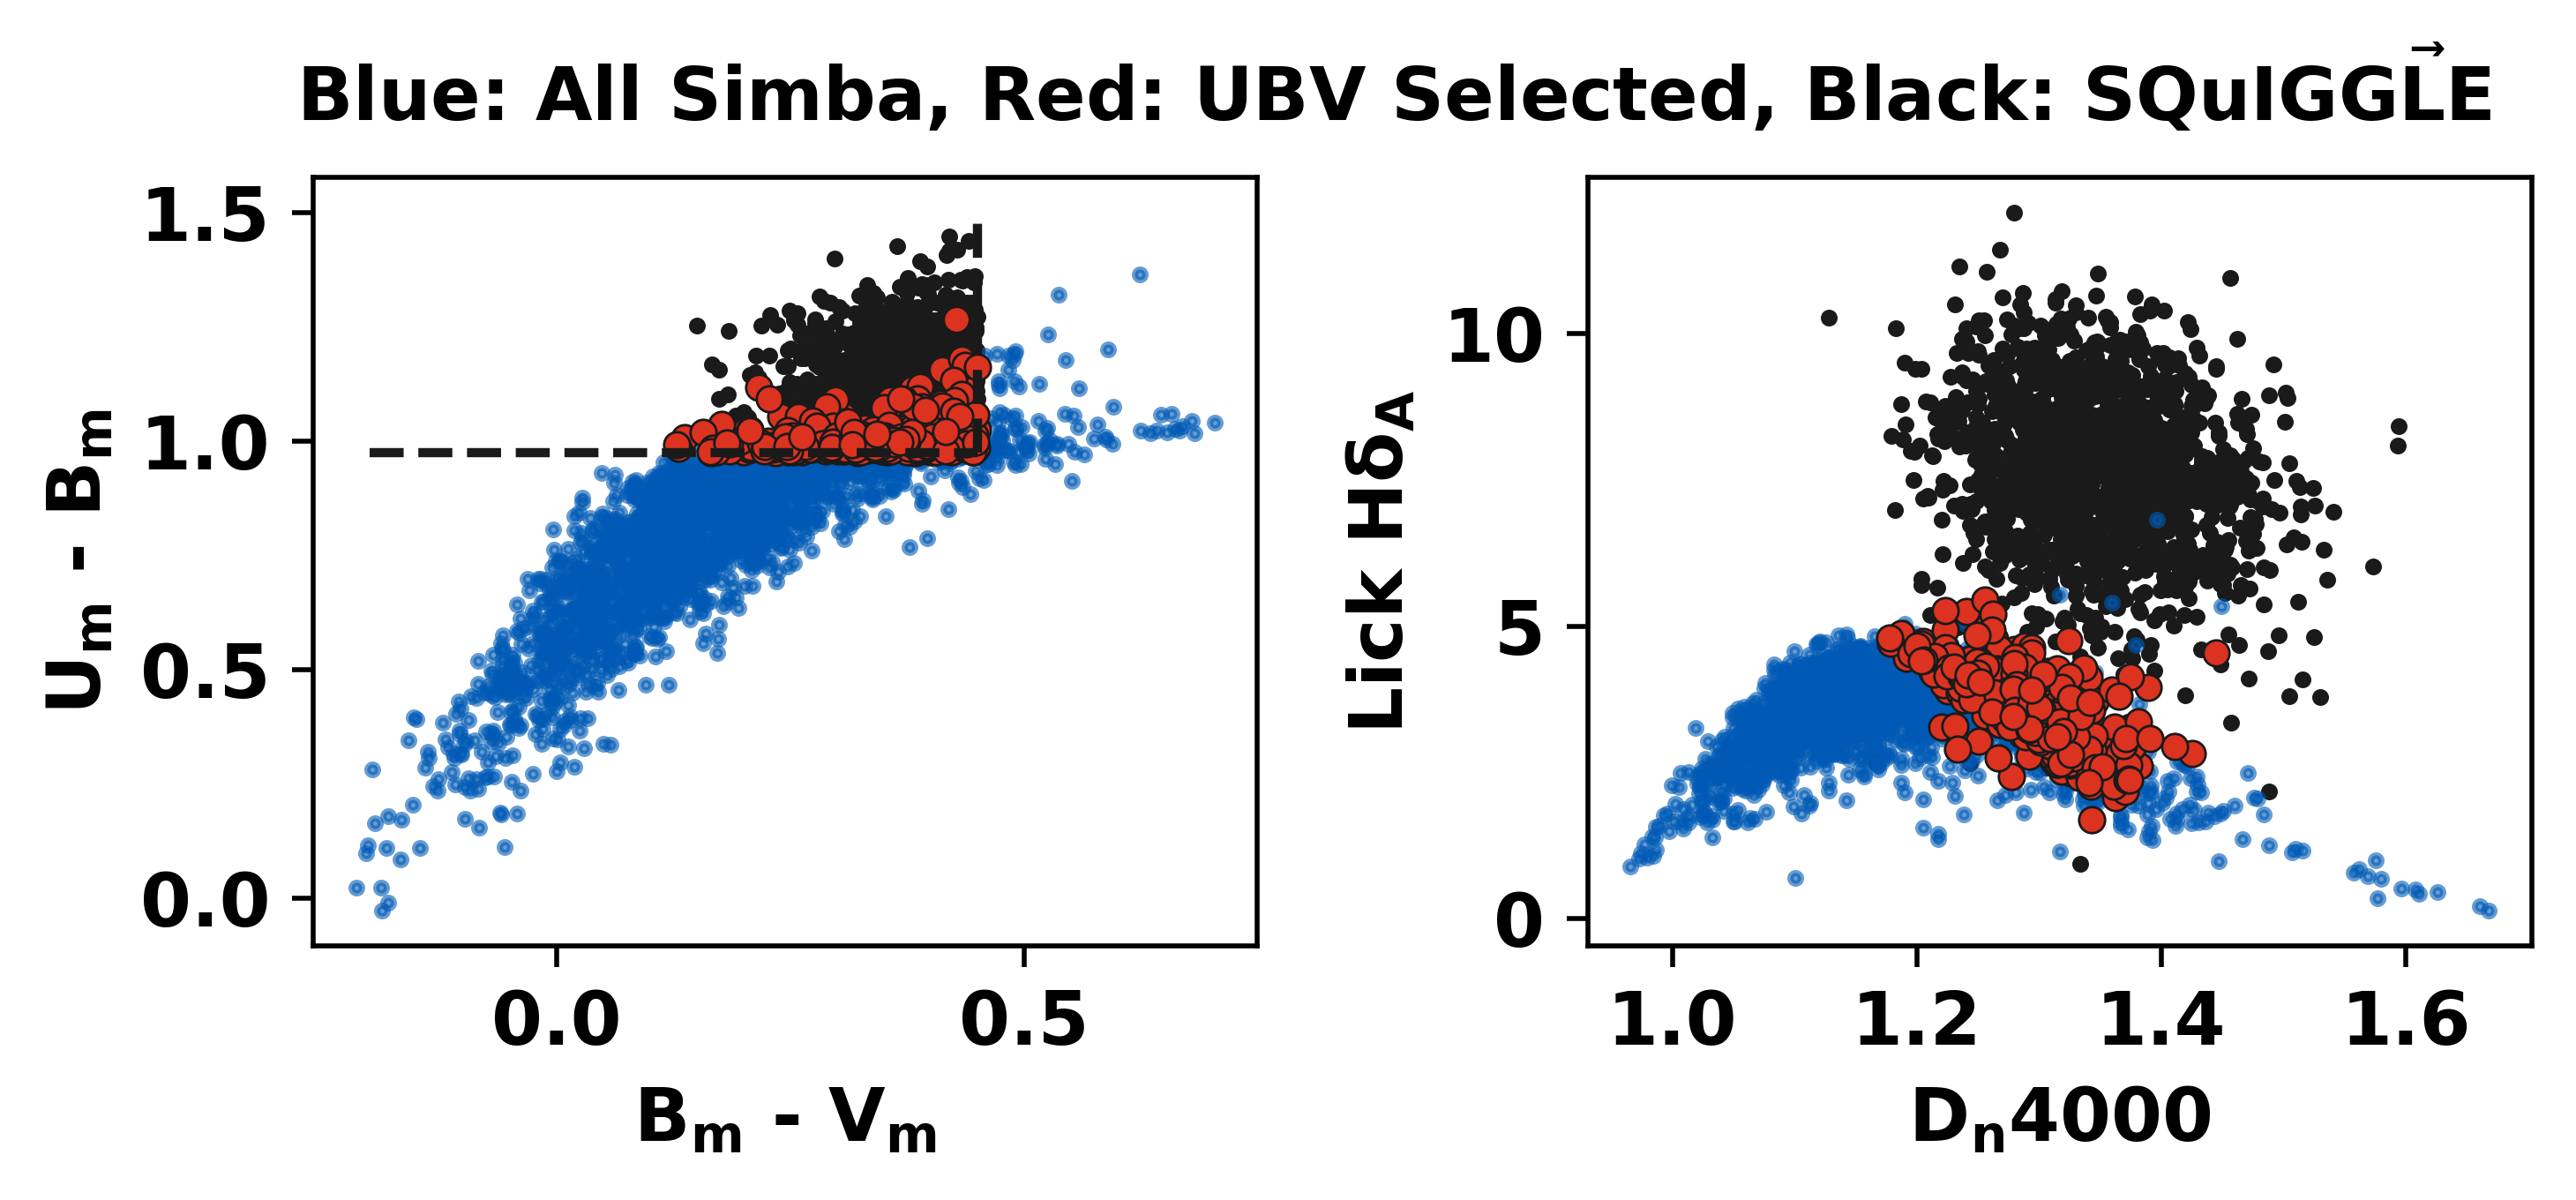
\includegraphics[width=.75\linewidth]{fig17_UBVSquiggle_z0p5.png}
    \caption{{\bf Same as \fig \ref{fig:UBV}, where red dots indicate those UBV-selected systems from \textbf{\textsc{SIMBA}} at $\bm{z=0.5}$, with the addition of galaxies from the SQuiGG$\bm{\vec{L}}$E survey (black points), shows how SQuiGG$\bm{\vec{L}}$E galaxies are generally redder than those UBV-selected \textbf{\textsc{SIMBA}} systems (red points).}  As in \fig \ref{fig:UBV}, the left-hand plot shows the galaxies in UBV space, defined by the medium-band rest-frame filters ($U_m$, $B_m$, and $V_m)$, designed to target the Balmer break and slope of the spectrum redward of the break \citep{suessSquiggle}. Right-hand plot shows the galaxies lick H$\delta_A$ index (i.e. H$\delta$ EW; which traces recent star formation) as a function of the 4000\r{A} break index (which probes the age of the stellar population).}
    \label{fig:ubvPlus}
\end{figure}

Secondly, we also see that the \squig\ galaxies (black points) also have relatively higher values of $B_m-V_m$ than the UBV-selected \simba systems (red points), implying that the \squig\ galaxies have redder (more positive) slopes in their spectra redwards/rightwards of the Balmer break then the UBV-selected systems in \simba.  It follows that the \squig\ galaxies will thus have a larger population of old, small and cool stars, while the \simba galaxies will be more young/hot/massive and dominated by recent star formation.  In fact, if we focused on the least burst-dominated \squig\ galaxy, with the same $U_m-B_m$ color as \simba, the biggest difference would be that the \simba galaxies are younger (lower/bluer $B_m-V_m$), and do not have the same old dominant population as in \squig.  Similarly, the fact that the \squig\ galaxies are on average older than those UBV-selected \simba galaxies is also why the \squig\ galaxies are shifted to higher values of D$_n$4000 in the right-panel of \fig\ref{fig:ubvPlus}.



Putting it all together, \fig\ref{fig:ubvPlus} implies that \simba UBV-selected galaxies are less burst-dominated then those in \squig, thus the \simba galaxies are more dominated by recent star formation, and contain more young, hot, and massive stars then in \squig.  This makes sense as by design, \simba is not meant to include bursty star formation.  The inability for \simba to produce `bursty' star formation largely stems from its subgrid treatment of the interstellar medium (ISM), which imposes a resolution-dependent temperature floor to prevent artificial fragmentation below the simulation’s mass resolution \citep{Springel03, mufasa, simba}. This effective equation of state stabilizes dense gas against collapse on unresolved scales, thereby smoothing star-formation variability in time.  

Now, the collective knowledge in this section can now be leveraged to understand the differences between the stacked spectra of our two samples.  In \fig\ref{fig:specStack} we show a combined stack of all $\sim$1,300 \squig\ galaxies as a solid black line, and the combined stack of our 409 UBV-selected ($z=0.5$) \simba galaxies as a solid red line, surrounded by a red shaded region indicating the 16th-84th percentile range of our spectra.  In general, comparing the two stacked spectra, given that each stack has been normalized at 4500\r{A}, shows that the \squig\ galaxies are generally redder than those in \simba\!\!, which also follows from the last paragraph in which we deduced that the \squig\ galaxies are also older.  As a confirmation of our intuition, since the \squig\ galaxies have larger values of $U_m-B_m$, it followed that they should also have a larger Balmer break, which can be seen in \fig\ref{fig:specStack}.  Similarly, the \squig\ galaxies also had generally larger values of $B_m-V_m$, which implied they had redder slopes redwards/rightwards of the Balmer break, which is also visually confirmed in \fig\ref{fig:specStack}.

\begin{figure}[H]
    \centering
    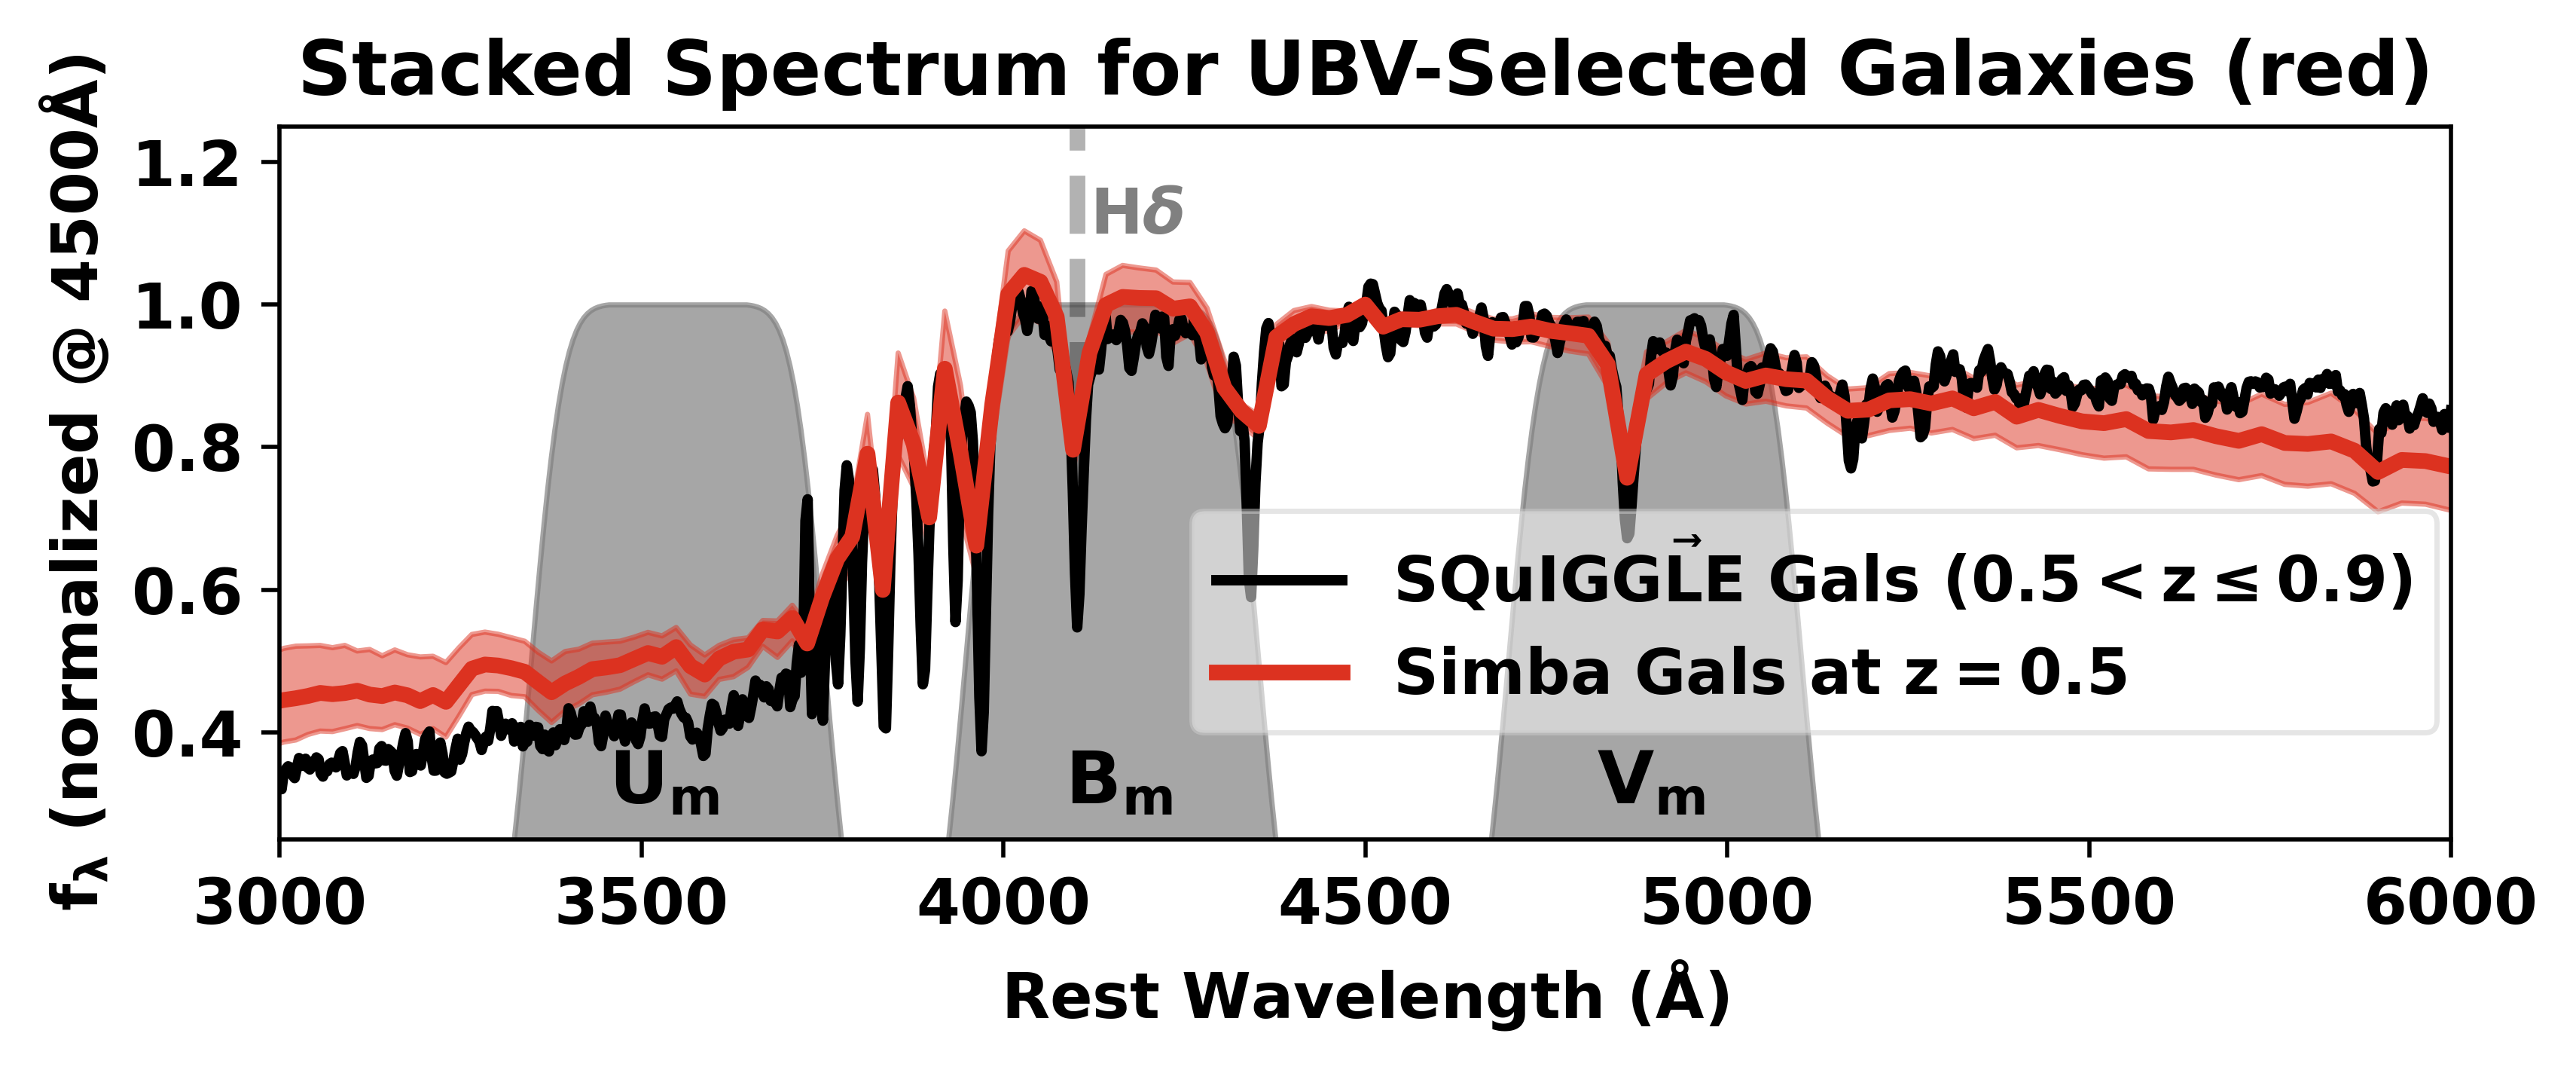
\includegraphics[width=.9\linewidth]{fig18_stackedSpec_z0p5(2).png}
    \caption{{\bf In general, SQuiGG$\bm{\vec{L}}$E galaxies are redder than those UBV-selected (\eq \ref{eq:UBVSelect}) galaxies from \textbf{\textsc{SIMBA}}.}  Spectral energy distributions (SEDs) for the two samples, stacked using the median and normalized at 4500\r{A}, are shown above.  The black line shows the result of $\sim$1,300 stacked \squig\ galaxies, while the red line shows the combined stack of 409 UBV-selected \simba galaxies, surrounded by a red shaded region indicating the 16th-84th percentile range of our spectra.  Additionally, we show as gray shaded regions the synthetic rest-frame $U_m$, $B_m$, and $V_m$ filters used to calculate the quantities shown in the left-panel of \fig \ref{fig:ubvPlus}.  Finally, we indicate the location of the Balmer H$\delta$ absorption line via a dashed vertical gray line at $\lambda=4101.734$\r{A}.  We see here that in comparison to \squig\ galaxies, the UBV-selected systems in \simba show a weaker Balmer break and stronger UV emission, suggesting that their stellar populations are more strongly influenced by recent star formation and therefore contain a larger fraction of young, hot, and massive stars.}
    \label{fig:specStack}
\end{figure}
\end{document}